\documentclass{book}

\usepackage{../Package/latexa}
\usepackage{../Package/algebra}
\usepackage{../Package/theorema}
\usepackage{../Package/diagramma}
\usepackage{../Package/categoria}

\newcommand{\qi}{\backsimeq_{\textsc{QI}}}
\newcommand{\ba}{\backsimeq_{\textsc{BA}}}
\newcommand{\normal}{\vartriangleleft}
\newcommand{\tm}{\subset}
\newcommand{\Stab}[2]{\textsf{Stab}_{#1}(#2)}
\newcommand{\Cay}[2]{\textsf{Cay}(#1,#2)}


\renewcommand{\A}{\mathbb{A}}
\renewcommand{\M}{\mathfrak{M}}
\newcommand{\Nc}{\mathcal{N}}


\renewcommand{\d}{\textsf{d}}
\renewcommand{\P}{\mathcal{P}}

\newcommand{\af}{\mathfrak{a}}
\newcommand{\Af}{\mathfrak{A}}
\renewcommand{\bf}{\mathfrak{b}}
\newcommand{\Bf}{\mathfrak{B}}
\newcommand{\cf}{\mathfrak{c}}
\newcommand{\Cf}{\mathfrak{C}}
\newcommand{\ff}{\mathfrak{f}}
\newcommand{\Ff}{\mathfrak{F}}
\newcommand{\pf}{\mathfrak{p}}
\newcommand{\Pf}{\mathfrak{P}}
\newcommand{\mf}{\mathfrak{m}}
\newcommand{\Mf}{\mathfrak{M}}
\newcommand{\qf}{\mathfrak{q}}
\newcommand{\Qf}{\mathfrak{Q}}

\renewcommand{\l}[1]{\overline{#1}}

\newcommand{\Ac}{\mathcal{A}}
\newcommand{\Rc}{\mathcal{R}}
\renewcommand{\O}{\mathcal{O}}

\newcommand{\Frob}{\textsf{Frob}}

\newcommand{\Leg}[2]{\left(\frac{#1}{#2}\right)}

\newcommand{\ric}{\textsf{ric}}
\newcommand{\g}{\mathfrak{g}}
\newcommand{\kf}{\mathfrak{k}}
\newcommand{\p}{\mathfrak{p}}
\newcommand{\m}{\mathfrak{m}}

\newcommand{\GL}{\textsf{GL}(n,\R)}
\newcommand{\glf}{\mathfrak{gl}(n,\R)}
\newcommand{\SO}{\textsf{SO}(n,\R)}
\newcommand{\so}{\mathfrak{so}(n,\R)}
\newcommand{\SL}{\textsf{SL}(n,\R)}
\newcommand{\slf}{\mathfrak{sl}(n,\R)}
\newcommand{\POS}{\textsf{Pos}(n,\R)}
\newcommand{\symm}{\textsf{symm}(n,\R)}
\newcommand{\of}{\mathfrak{o}}
\renewcommand{\epsilon}{\varepsilon}

\usepackage{enumerate}

\makeindex

\begin{document}

\title{
\begin{huge}
Geometrie der Mannigfaltigkeiten\\
\end{huge}
\begin{large}
Kurzskript, SS 17
\end{large}}


\author{Ak\i n}
\maketitle
\renewcommand{\i}{^{-1}}

%Das folgende Kurzskript orientiert sich an einer Vorlesung, die im Wintersemester 2016 / 2017 in Heidelberg gehalten wurde. Für alle Fehler im Text trägt ausschließlich der Autor die Verantwortung.

\setcounter{tocdepth}{1}
\tableofcontents

% % % Vorlesung 1
\newpage
\chapter{Hyperbolische Modelle}
\section{Das Hyperboloidenmodell}
\Def{}
Definiere die \df{Lorentzform} auf $\R^{n+1}$ durch
\[ \shrp{x,y} := x_1y_1 + \ldots + x_{n}y_n - x_{n+1} y_{n+1} \]
Ein Vektor$x \in \R^{n+1}$ heißt
\begin{align*}
\left\lbrace \begin{aligned}
\text{\df{zeitartig}, falls } &\shrp{x,x} < 0\\
\text{\df{lichtartig}, falls } &\shrp{x,x} = 0\\
\text{\df{raumartig}, falls } &\shrp{x,x} > 0
\end{aligned} \right.
\end{align*}
Definiere das \df{Hyperboloidenmodell} von $\H^n$ durch
\[ I^n = \set{p \in \R^{n+1}}{\shrp{p,p} = -1, p_{n+1 > 0}} \]
\Prop{}
$I^n$ ist eine Riemannsche Mannigfaltigkeit.
\begin{Beweis}{}
Definiere $f : \R^{n+1} \pfeil{} \R$ durch $x \mapsto \shrp{x,x}$. Dann ist $\d f_p(v) = 2\shrp{v,p}$. Ergo ist $\d f_p$ surjektiv für alle $p \in M :=f\i(-1)$. Ergo ist $M$ eine glatte Hyperfläche von $\R^{n+1}$.\\
Ferner ist
\[ T_pM = \Ker ~\d f_p  = \set{v \in \R^{n+1}}{\shrp{p,v} = 0} = p^\bot \]
Da $p$ zeitartig ist, ist $\shrp{\_, \_}$ auf $T_pM$ positiv definit. $I^n$ ist nun gerade die obere Zusammenhangskomponente von $M$.
\end{Beweis}

\Lem{}
Definiere
\[ O(n,1) = \set{A \in \R^{n+1\times n + 1}}{ \shrp{v,w} = \shrp{Av, Aw} }\]
und
\[ O(n,1)^+ = \set{A \in O(n,1)}{A (I^n) \subset I^n } \]
Dann ist $O(n,1)^+$ eine Index-2-Gruppe von $O(n,1)$ und
\[ Isom(I^n) = O(n,1)^+ \]
Ferner gilt
\[ Isom(S^n) = O(n) \text{ und } Isom(\R^n) = \set{x\mapsto Ax + b}{A \in O(n), b\in \R^n } \]


\Prop{}
Die $k$-dimensionalen, vollständigen, total geodätischen, zusammenhängenden Riemannschen Untermannigfaltigkeiten von $I^n$ sind genau die Schnitte
\[ I^n \cap W^{k+1}\]
wobei $W^{k+1}$ ein $k+1$-dimensionaler Untervektorraum von $\R^{n+1}$ ist, der keinen leeren Schnitt mit $I^n$ hat.\\
Folgende Aussagen sind für einen $k+1$-dimensionalen Untervektorraum von $\R^{n+1}$ äquivalent:
\begin{enumerate}[]
	\item $W^{k+1}\cap I^n \neq \emptyset$
	\item $W^{k+1}$ besitzt einen zeit-ähnlichen Vektor
	\item $\shrp{\_,\_}$ besitzt auf $W^{k+1}$ die Signatur $(k,1)$
\end{enumerate}

\Bem{}
Ein $k$-Unterraum von $I^n$ ist isometrisch zu $I^k$.

\Prop{}
Jede nach Bogenlänge parametrisierte Geodäte von $I^n$ ist von der Gestalt
\[ \gamma(t) = \cosh(t) \gamma(0) + \sinh(t)\dot{\gamma}(0) \]

\Kor{}
$H^n$ ist vollständig.

\section{Die Poincare Scheibe}
\Lem{Poincare-Scheiben-Modell}
Definiere die \df{Poincare-Scheibe} durch
\[D^n = \set{x \in \R^n}{\norm{x} < 1} \]
und folgenden Diffeomorphismus
\begin{align*}
p : I^n & \Pfeil{} D^n\\
(x_1, \ldots, x_n, x_{n+1}) & \longmapsto \frac{1}{x_{n+1} + 1} (x_1,\ldots, x_n) 
\end{align*}
Dann ist die Metrik auf $D^n$ gerade gegeben durch
\[ g^D_x = \klam{\frac{2}{1 - \norm{x}^2}}^2g^E_x \]
wobei $g^E$ die euklidische Metrik von $\R^n$ bezeichnet.
\begin{Beweis}{}
	Die Umkehrabbildung von $p$ ist gerade
	\[ p\i(x) = \frac{(2x, 1 + \norm{x}^2)}{1 - \norm{x}^2} \]
	Ihre Derivation ist
	\[ \d_xp\i(u) = \frac{ 2 (u (1 - \norm{x}^2) + 2 x(x|u), 2 (x|u) )}{ (1 - \norm{x}^2)^2 } \]
	Es gilt
	\[ \shrp{d_xp\i(u), d_xp\i(u)} = (\frac{2}{1 - \norm{x}})^2 \norm{u}^2 \]
	Da $p\i$ eine Isometrie sein soll und das Verhalten einer Metrik durch ihre Norm bestimmt ist, folgt nun
	\[ g^D_x = g^I_{p\i(x)} \circ \d_xp\i  = \klam{\frac{2}{1 - \norm{x}^2}}^2g^E_x \]
\end{Beweis}

\Def{}
Ein Diffeomorphismus
\[ f : (M,g) \Pfeil{} (N,h) \] 
heißt \df{konform}, falls eine glatte Funktion $f : M \pfeil{} \R_{>0}$ existiert, sodass
\[ f^*(h_{f(p)}) = \lambda(p)\cdot g_p  \]

\Bem{}
Die Poincare-Scheibe ist ein konformes Modell von $\H^n$, d.\,h., $(D^n, g^E)$ und $(D^n, g^D)$ sind zueinander konform.\\
Daraus folgt nun insbesondere, dass Winkel von sich schneidenden Geodäten in $(D^n, g^D)$ genauso wie in $(D^n, g^E)$ gemessen werden dürfen.

\Lem{}
Die $k$-dimensionalen, vollständigen, zusammenhängenden, total geodätischen Untermannigfaltigkeiten der Poincare-Scheibe sind ihre Schnitte mit $k$-Sphären und $k$-Ebenen von $\R^n$, die orthogonal zum Rand der Poincare-Scheibe liegen.

\Def{}
Sei $S_{p}(r) \subset \R^n$ eine Sphäre mit Radius $r$ um $p$. Definiere die \df{Inversion} an $S_p(r)$ durch
\begin{align*}
\phi : \R^n\setminus\{p\} & \Pfeil{} \R^n\setminus\{p\}\\
x & \longmapsto p + r^2\frac{x- p}{\norm{x-p}^2}
\end{align*}
\Prop{}
Jede Inversion ist \df{anti-konform}, d.\,h. konform und Orientierung umkehrend, und bildet Sphären und Ebenen auf Sphären und Ebenen ab.

\section{Das obere Halbraum-Modell}
\Def{}
Das \df{obere Halbraum-Modell}
\[ H^n = \set{x \in \R^{n}}{x_n > 0} \]
ergibt sich durch eine Inversion der Poincare-Scheibe an der Sphäre
\[ S = S_{(0,\ldots,0,-1)}(\sqrt{2}) \]
Insofern ist die obere Halbebene ein konformes Modell von $\H^n$.

\Prop{}
Die $k$-Ebenen von $H^n$ sind die $k$-Ebenen und $k$-Sphären von $\R^n$, die orthogonal zu $\partial H^n$ sind.

\Prop{}
Die Metrik auf $H^n$ ist gegeben durch
\[ g_x^H =  \frac{1}{x_n^2} g^E \]


\Prop{}
Folgende Abbildungen sind Isometrien von $H^n$:
\begin{enumerate}[1.)]
\item Horizontale Translationen:
\begin{align*}
x \longmapsto x + (b_1,\ldots, b_{n-1}, 0)
\end{align*}
\item Dilationen:
\[ x \longmapsto x \cdot \lambda \]
\item Inversionen an Sphären orthogonal zu $\partial H^n$
\end{enumerate}

\Prop{}
Die Isometrien der Poincare-Scheibe und der oberen Halbebene werden durch Inversionen an Sphären und Reflektion an Euklidischen Ebenen, die alle orthogonal zum Rand stehen, erzeugt.
\Prop{}
In den konformen Modellen sind Kugeln genau die euklidischen Kugeln mit exzentrischen Mittelpunkten.

\section{Die Kleinsche Scheibe}
\Def{}
Die \df{Kleinsche Ebene} besitzt dieselbe Trägermenge $K^n = D^n$ wie die Poincare-Scheibe. Allerdings entsteht die Kleinsche-Ebene durch einen Diffeomorphismus
\begin{align*}
I^n & \Pfeil{} K^n\\
x & \longmapsto \frac{(x_1,\ldots,x_n)}{x_n}
\end{align*}
Die Kleinsche Scheibe ist nicht konform, weswegen ihre Winkel nicht durch eine euklidische Einbettung gemessen werden können. Allerdings sind ihre Geodäten genau die Geraden des $\R^n$.

\section{Ränder}
\Def{}
Zwei nach Bogenlänge parametrisierte Geodäten $\alpha, \beta : [0, \infty) \pfeil{} M$ heißen \df{asymptotisch äquivalent}, falls die Funktion
\[ t \longmapsto d(\alpha(t), \beta(t)) \]
beschränkt ist.\\
Asymptotisch äquivalent Sein ist eine Äquivalenzrelation auf der Menge aller geodätischer Halbgeraden.\\
Teilt man diese Relation heraus, erhält man den \df{Rand} $\partial M$ einer Mannigfaltigkeit $M$. Insbesondere schreibt man
\[ \overline{M} = M \cup \partial M \]

\Prop{}
Es gibt eine Bijektion zwischen $\partial D^n$ als Rand einer Mannigfaltigkeit und $S^{n-1}$.\\
Da ferner $\overline{D^n}$ eine naheliegende Topologie besitzt, können wir diese auf $\overline{\H^n}$ zurückführen.
\begin{Beweis}{}
	Sei $\gamma : [0, \infty) \pfeil{} D^n$ ein geodätischer Strahl. Da $\gamma$ sich orthogonal mit $S^{n-1}$ im Unendlichen schneiden muss, folgt
	\[ \lim\limits_{t \pfeil{} \infty} \gamma(t) \in S^{n-1} \]
	Hierdurch erhalten wir eine surjektive Abbildung
	\[ R(\gamma) :=  \lim\limits_{t \pfeil{} \infty} \gamma(t) \]
	Wir müssen nun zeigen, dass zwei nach Bogenlänge parametrisierte Strahlen $\gamma$, $\beta$ unter $R$ genau dann dasselbe Bild haben, wenn sie asymptotisch äquivalent sind.\\
Wir transformieren das Problem zu einem Problem auf $H^n$ und rechnen die geforderte Eigenschaft dort konstruktiv nach.
\end{Beweis}

\Bem{}
Man kann auch alternativ wie folgt eine Basis der Topologie von $\overline{\H^n}$ definieren: Dazu nimmt man alle offenen Mengen von $\H^n$ und schmeißt alle Mengen der Gestalt
\[ \{ \alpha(t) \in \H^n~|~ \alpha(0) = \gamma(0), \dot{\alpha}(0)  \in V ,t > r\} \cup \set{ [\alpha] \in \partial \H^n }{\alpha(0) = \gamma(0),\dot{\alpha}(0)  \in V} \]
für alle $[\gamma] \in \partial \H^n, V \subseteq_o T_{\gamma(0)}M, r > 0$. Die hierdurch entstehende Topologie stimmt der durch obige Proposition überein.

\Prop{}
Seien $S,S'$ zwei geodätisch vollständige Teilräume von $\H^n$. Dann tretet genau einer der folgenden Fälle ein:
\begin{itemize}
	\item $S$ und $S'$ sind \df{inzident}, d.\,h., $S\cap S'\neq \emptyset$.
	\item $S$ und $S'$ sind \df{asymptotisch parallel}, d.\,h., $S\cap S' = \emptyset$ und $d(S, S') = 0$. Ferner ist dann $\overline{S} \cap \overline{S'}$ ein Punkt in $\H^n$ und existiert keine Geodäte, die zu beiden Räumen orthogonal ist.
	\item $S$ und $S'$ sind \df{ultra-parallel}, d.\,h., $\overline{S}\cap \overline{S'} = \emptyset$ und $d(S, S') > 0$. In diesem Fall existiert genau eine Geodäte, die orthogonal zu beiden Teilräumen steht und den Abstand zwischen beiden realisiert.
\end{itemize}
\begin{Beweis}{}
	Enthält $\overline{S} \cap \overline{S'}$ mindestens zwei Punkte, so enthält der Schnitt auch eine Geodäte zwischen beiden Punkten. Wir können also annehmen, dass sich $S$ und $S'$ wenn überhaupt nur im Unendlichen schneiden und dort höchstens einen Schnittpunkt haben.\\
	Besteht $\overline{S} \cap \overline{S'}$ aus genau einem Punkt, so können wir die Situation in den $H^n$ transformieren und fordern, dass der gemeinsame Schnittpunkt gerade $\infty$ ist. In diesem Fall stehen $S$ und $S'$ parallel zur imaginären Achse, weswegen die Eigenschaften des zweiten Falles folgen.\\
	Im zweiten Fall finden wir $x\in S, x' \in S'$ mit $d(x,x') = d(S, S')$, da $\overline{S}$ und $\overline{S'}$ kompakt sind. Die Geodäte, die $x$ und $x'$ verbindet, muss orthogonal sein, da wir sie sonst verschieben könnten, um den Abstand zwischen $S$ und $S'$ zu minimieren. Es kann keine weitere Geodäte zwischen $S$ und $S'$ mit Abstand $d(S, S')$ geben, da wir sonst einen flachen Bereich gefunden hätten.
\end{Beweis}

\Lem{}
Eine Isometrie $\phi : \H^n \pfeil{} \H^n$ lässt sich zu einem Homöomorphismus $\overline{\phi} : \overline{\H^n} \pfeil{} \overline{\H^n} $ fortsetzen. $\phi$ ist durch $\overline{\phi}_{\partial \H^n}$ eindeutig festgelegt.

\section{Isometrien}
\Prop{}
Sei $\phi : \H^n \pfeil{} \H^n$ eine nichttriviale Isometrie. Dann tritt genau einer der folgenden Fälle ein:
\begin{itemize}
	\item $\phi$ ist \df{elliptisch}, d.\,h., $\phi$ hat einen oder mehrere Fixpunkte in $\H^n$.
	\item $\phi$ ist \df{parabolisch}, d.\,h., $\phi$ hat keinen Fixpunkt in $\H^n$, aber genau einen in $\partial \H^n$.
	\item $\phi$ ist \df{hyperbolisch}, d.\,h., $\phi$ hat keinen Fixpunkt in $\H^n$, aber genau zwei in $\partial \H^n$.
\end{itemize}
\begin{Beweis}{}
Wir können $\overline{\phi}$ als einen Homöomorphismus von $\overline{D^n}$ auf sich selbst auffassen. Nach Brauers Fixpunktsatz muss $\phi$ dann mindestens einen Fixpunkt haben. Hat $\phi$ keinen Fixpunkt in $D^n$ aber mindestens drei auf dem Rand, so fixiert $\phi$ jeden Punkt in $\H^n$, da jeder Punkt in $D^n$ durch seine Winkel zu den drei verschiedenen Randpunkten eindeutig determiniert ist.
\end{Beweis}

\Def{}
Eine hyperbolische Isometrie fixiert zwei Randpunkte und damit auch die Geodäte, die zwischen beiden verläuft. Diese eindeutig bestimmte Geodäte nenne wir die \df{Achse} von $\phi$.

\Def{}
Eine \df{Horosphäre} $S \subset \overline{\H^n}$ um den Punkt $p \in \partial H^n\setminus\{\infty\}$ ist eine $n-1$-dimensionale euklidische Sphäre, die $\partial H^n$ tangential in $p$ schneidet. Eine Horosphäre um $\infty$ ist eine $n-1$-dimensionale euklidische Hyperebene, die orthogonal zur imaginären Achse steht.\\
Beide Horosphären sind flache Untermannigfaltigkeiten mit der Eigenschaft, dass jede Geodäte, die ihr Zentrum verlässt, die Horosphäre orthogonal schneidet.

\Prop{}
Wir stellen Punkte aus $H^n$ in der Form $(x,t)$ dar. Sei $\phi$ eine nichttriviale Isometrie von $\H^n$.
\begin{itemize}
	\item Ist $\phi$ elliptisch mit Fixpunkt $0 \in D^n$, so gibt es ein $A \in O(n)$, sodass sich $\phi$ darstellen lässt durch
	\begin{align*}
\phi:	D^n & \Pfeil{} D^n\\
	x & \longmapsto Ax
	\end{align*}
	\item Ist $\phi$ parabolisch mit Fixpunkt $\infty \in \partial H^n$, so gibt es $A \in O(n-1)$ und $b\in \R^{n-1}$, sodass
	\begin{align*}
\phi:	H^n & \Pfeil{} H^n\\
	(x,t) & \longmapsto (Ax + b, t)
	\end{align*}
	\item Ist $\phi$ hyperbolisch mit Fixpunkten $0,\infty \in \partial H^n$, so gibt es ein $\lambda > 0, \neq 1$ und ein $A\in O(n-1)$, sodass
		\begin{align*}
	\phi:	H^n & \Pfeil{} H^n\\
	(x,t) & \longmapsto (\lambda Ax, \lambda t)
	\end{align*}
\end{itemize}
\begin{Beweis}{}
Der elliptische Fall ist klar.\\
Sei der zweite Fall gegeben. Ist $O$ eine Horosphäre um $\infty$, so muss $\phi(O)$ wieder eine Horosphäre um $\infty$ liefern. Dann gibt es ein $(x,t) \in O$, sodass $\phi(x,t) = (x, t')$. Ist $t' \neq t$, so erhält $\phi$ eine Geodäte durch $(x,t)$ und $\infty$ und ist nicht mehr parabolisch. Ergo ist $\phi(O) = O$. D.\,h., $\phi$ ist auf jeder Horosphäre um $\infty$ durch eine euklidische Isometrie gegeben.\\
Sei nun der dritte Fall gegeben. $\phi$ erhält die imaginäre Achse, ergo gibt es ein $\lambda$ mit $\phi(0,1) = (0, \lambda)$. Setzt man $\psi(x,t) = \lambda\i \phi(x,t)$, so gibt es ein $A\in O(n-1)$ mit
\[ \d_{(0,1)} \psi = \klam{
\begin{matrix}
A & 0\\
0 & 1
\end{matrix}
} \]
womit folgt
\[ \psi(x,t) = (Ax,t) \]
\end{Beweis}

\Def{}
Für eine Isometrie $\phi : M \pfeil{} M$ sei die \df{Versetzung} definiert durch
\begin{align*}
d(\phi) := \inf_{p\in M}d(p, \phi(p))
\end{align*}

\Kor{}
\begin{itemize}
	\item Eine elliptische Isometrie hat eine Versetzung von 0, die an ihren Fixpunkten verwirklicht wird.
	\item Eine parabolische Isometrie hat eine Versetzung von 0, die nirgendwo realisiert wird, und fixiert jede Horosphäre um ihren Fixpunkt.
	\item Eine hyperbolische Isometrie hat eine Versetzung von $d > 0$, die genau auf ihrer Achse realisiert wird.
\end{itemize}

\section{Möbiusgeschichten}
\Def{}
Es bezeichne $S = \C \cup \infty$ die \df{Riemannsche Zahlenkugel}. Die Gruppe $PSL_2(\C)$ agiert auf $S$ durch die \df{Möbiustransformation}
\[ \klam{
\begin{matrix}
a & b\\
c & d
\end{matrix}
}.z := \frac{az + b}{cz + d} \]
Die Möbiustransformation ist ein orientierungserhaltender Diffeomorphismus auf $S$.\\
Die \df{Anti-Möbiustransformation} gegeben durch
\[ \klam{
	\begin{matrix}
	a & b\\
	c & d
	\end{matrix}
}.z := \frac{a\overline{z} + b}{c\overline{z} + d} \]
ist ein orientierungsumkehrender Diffeomorphismus auf $S$.\\
Unter $Conf(S) \subset Diffeo(S)$ verstehen wir die Menge aller Möbius- und Anti-Möbiustransformationen, die durch Elemente aus $PSL_2(\C)$ induziert werden.

\Prop{}
Inversionen entlang Sphären und Spiegelungen entlang Geraden sind beides Anti-Möbiustransformationen und erzeugen $Conf(S)$.

\Lem{}
Betrachte
\[ H^2 = \set{ x + iy}{x \in \R, y > 0} \]
und setze
\[ Conf(H^2) = \set{\phi \in Conf(S)}{\phi(H^2) \subseteq H^2} \]
Dann ist jede Transformation aus $Conf(H^2)$ induziert durch eine Matrix mit reellen Einträgen, deren Determinante gleich 1 ist, falls die Transformation orientierungserhaltend ist, anderenfalls -1 ist.\\
Es gilt
\[ Conf^+(H^2) = PSL_2(\R) \]

\Prop{}
Inversionen entlang Kreisen und Reflexionen entlang Geraden, die beide orthogonal zu $\R$ sind, generieren $Conf(H^2)$.
\Kor{}
\[ Conf(H^2) = Isom(H^2) \]

\Prop{}
Eine nichttriviale Transformation $A \in PSL_2(\R)$ ist
\begin{itemize}
	\item elliptisch, falls $\bet{tr(A)} < 2$
	\item parabolisch, falls $\bet{tr(A)} = 2$
	\item hyperbolisch, falls $\bet{tr(A)} > 2$
\end{itemize}

\Prop{}
Da $\partial H^3 = S$, gilt
\[ Isom(H^2) = Conf(S) \]

\Prop{}
Eine nichttriviale Transformation $A \in PSL_2(\C)$ ist
\begin{itemize}
	\item elliptisch, falls $tr(A) \in (-2, 2)$
	\item parabolisch, falls $tr(A) = \pm 2$
	\item hyperbolisch, falls $tr(A) \in \C\setminus [-2, 2]$
\end{itemize}

\Prop{}
Die Distanzfunktion ist auf $\H^n$ \df{strikt konvex}, d.\,h., für je zwei nach Bogenlänge parametrisierte, disjunkte Geodäten $\alpha, \beta : \R \pfeil{} \H^n$ gilt
\[ d(\alpha(t  x_1 + (1-t)  y_1), \beta(t  x_2 + (1-t)  y_2) ) < t  d(\alpha(x_1), \beta(x_2)) + (1-t)  d(\alpha(y_1), \beta(y_2) ) \]
für alle $x_1 \neq y_1, x_2 \neq y_2, t \in (0,1)$.
\begin{Beweis}{}
	Da die Distanzfunktion stetig ist, genügt es die Aussage für $t = \frac{1}{2}$ zu zeigen, also
	\[ d(\alpha(\frac{x_1 + y_1}{2}), \beta(\frac{x_2 + y_2}{2})) < \frac{d(\alpha(x_1), \beta(x_2) ) + d(\alpha(y_1), \beta(y_2))}{2}  \]
	Setze
	\[ m:= \alpha(\frac{x_1 + y_1}{2})  \text{ und }n:= \beta(\frac{x_2 + y_2}{2}) \]
	Für einen Punkt $p \in \H^n$ bezeichne $s_p$ die Punktspiegelung bei $p$. Dies ist eine globale Isometrie. Für zwei verschiedene Punkte $p,q$ ist $s_p \circ s_q$ eine orientierungserhaltende Isometrie. Insbesondere ist diese hyperbolisch, denn ist $l$ die Geodäte, die $p$ und $q$ enthält, so wird jeder Punkt auf $l$ um $2d(p,q)$ entlang $l$ bewegt.\\
	Setze nun
	\[ \tau = s_n \circ s_m \]
	Dann gilt
	\begin{align*}
	d(\alpha(x_1), \tau(\alpha(x_1)) ) & \leq d(\alpha(x_1), \beta(x_2) ) + d( \beta(x_2), \tau(\alpha(x_1)) )\\
	&=d(\alpha(x_1), \beta(x_2) ) + d(  s_n(\beta(y_2))  , s_n(\alpha(y_1))  )\\
		&=d(\alpha(x_1), \beta(x_2) ) + d(  \beta(y_2)  , \alpha(y_1)  )\\
	\end{align*}
	Da $\alpha(x_1)$ nicht auf der hyperbolischen Achse von $\tau$ liegt, gilt ferner
		\begin{align*}
2d(m,n) &= d(m, \tau(m))\\
&< d(\alpha(x_1), \tau(\alpha(x_1)))\\
&\leq d(\alpha(x_1), \beta(x_2) ) + d(  \beta(y_2)  , \alpha(y_1)  )
	\end{align*}
\end{Beweis}

\chapter{Werkzeuge der Hyperbolischen Mannigfaltigkeiten}
\section{Hyperbolische Mannigfaltigkeiten}
\Def{}
Eine Mannigfaltigkeit heißt \df{hyperbolisch}, wenn sie durch offene, lokal isometrische Karten $\phi : U \pfeil{} \H^n$ überdeckt wird und zusammenhängend ist.

\Satz{}
Eine hyperbolische, einfach zusammenhängende, vollständige Mannigfaltigkeit ist isometrisch zu $\H^n$.
\begin{Beweis}{Skizze}
	Wir konstruieren eine lokal isometrische Abbildung $D : M \pfeil{} \H^n$. Zuerst wählen wir eine Karte $ U \pfeil{} \H^n$ und einen Punkt $p \in U$. Für ein beliebiges $q \in M$ wählen wir einen Weg $\gamma : p \mapsto q$ und überdecken diesen Weg mit endlich vielen hyperbolischen, kompatiblen Karten. Dadurch können wir $q$ einem Punkt aus $D(q) \in \H^n$ zuordnen.\\
	Um die Wohldefiniertheit von $D$ zu zeigen, zeigt man zuerst, dass die Wahl der Karten, die $\gamma$ überdecken unerheblich für die Wahl des Bildpunktes $D(q)$ sind.\\
	Danach zeigt man, dass $D(q)$ unabhängig von der Wahl des Weges $\gamma:p\mapsto q$ ist. Denn ist $H : \gamma \sim \gamma'$ eine Homotopie mit fixierten Endpunkten, so ist $D(H)$ ebenfalls eine Homotopie mit fixierten Endpunkten.\\
	Da $D$ lokal isometrisch und $M$ geodätisch vollständig ist, ist $D$ surjektiv. Da $\H^n$ ferner einfach zusammenhängend ist, ist $D$ injektiv. 
\end{Beweis}

\Kor{}
Ist $M$ eine hyperbolische, einfach zusammenhängende Mannigfaltigkeit, so gibt es eine lokal isometrische Abbildung $D : M \pfeil{} \H^n$, die sogenannte \df{Entfaltung}, die eindeutig bis auf Nachschaltung einer Isometrie auf $\H^n$ ist.

\newpage
\Prop{}
Sei $M$ eine hyperbolische Mannigfaltigkeit und $D : M \pfeil{} \H^n$ eine lokale Isometrie. Für jedes $g\in Isom(M)$ existiert genau ein $\rho(g) \in Isom(\H^n)$, sodass folgendes Diagramm kommutiert
\begin{center}
	\begin{tikzpicture}
	\node (M1) at (0,2) [] {$M$};
	\node (H1) at (4,2) [] {$\H^n$};
	\node (H2) at (4,0) [] {$\H^n$};
	\node (M2) at (0,0) [] {$M$};
	
	\draw [->] (M1) -> (H1) node[midway, above] {$D$};
	\draw [->] (M2) -> (H2) node[midway, above] {$D$};
	\draw [->] (M1) -> (M2) node[midway, right] {$g$};
	\draw [->] (H1) -> (H2) node[midway, right] {$\rho(g)$};
	\end{tikzpicture}
\end{center}
Die Abbildung $\rho : Isom(M) \pfeil{} Isom(\H^n)$ ist eine Gruppenhomomorphismus und heißt die \df{Holonomie} zu $D$.

\Bem{}
Sei $M$ eine hyperbolische, vollständige Mannigfaltigkeit. Ist $\widetilde{M} \pfeil{} M$ die universelle Überlagerung von $M$, so ist $\widetilde{M}$ hyperbolisch, vollständig und einfach zusammenhängend und deswegen isometrisch zu $\H^n$. Wir erhalten also eine lokal isometrische Überlagerung $\H^n \pfeil{} M$ und wissen dadurch
\[ \pi_1(M) = Deck(\H^n \pfeil{} M) \subseteq Isom(\H^n) \]

\section{Vollständige Hyperbolische Mannigfaltigkeiten}
\Def{}
Sei $G$ eine Gruppe, die auf einen topologischen Raum $X$ wirkt. Diese Wirkung heißt \df{eigentlich diskontinuierlich}, falls es für jedes Paar von zwei verschiedenen Punkten $x,y \in X$ Umgebungen $U_x, U_y$ existieren, sodass
\[ \#\set{g \in G}{g.U_x \cap U_y \neq \emptyset} < \infty \]
Die Wirkung heißt \df{frei}, falls jedes nichttriviale $g\in G$ fixpunktfrei auf $X$ wirkt.

\Lem{}
Wirkt $\Gamma \subset Isom(\H^n)$ frei und eigentlich diskontinuierlich auf $\H^n$, so besitzt $\H^n / \Gamma$ genau eine Struktur als hyperbolische, vollständige Mannigfaltigkeit, durch die $\H^n \pfeil{} \H^n/\Gamma$ zu einer \df{Riemannschen Überlagerung}, d.\,h., lokal isometrischen Überlagerung wird.

\Prop{}
Jede vollständige, hyperbolische Mannigfaltigkeit ist isometrisch zu $\H^n / \Gamma$ für eine passende Gruppe $\Gamma \subset Isom(\H^n)$, die frei und eigentlich diskontinuierlich wirkt.

\Bem{}
$\Gamma \subset  Isom(\H^n)$ wirkt genau dann eigentlich diskontinuierlich, wenn $\Gamma$ diskret ist.
\begin{Beweis}{}
	$\Gamma$ wirke eigentlich diskontinuierlich. Seien $x,y \in \H^n$, dann gibt es Umgebungen $U_x, U_y$, sodass nur endlich viele Elemente aus $\Gamma$ $U_x$ über $U_y$ bewegen.\\
	Definiert man die Abbildung
	\begin{align*}
	\phi : \Gamma& \Pfeil{} \H^n\\
	g & \longmapsto g(x)
	\end{align*}
	so besitzt die offene Menge $\phi\i(U_x)$ nur endlich viele Elemente. Ergo besitzt jeder Punkt aus $\Gamma$ eine endliche Umgebung.\\
	Sei $\Gamma$ nun diskret. Seien $x,y \in \H^n$ zwei verschiedene Punkte. Definiere $A:= \set{g \in \Gamma}{g.U_x \cap U_y \neq \emptyset}$. Indem wir $U_x$ und $U_y$ sukzessive kleiner machen, finden wir eine Folge in $\Gamma$, die durch ein Kompaktum beschränkt wird. Da $\Gamma$ endlich ist, muss dieses Kompaktum endlich sein.
\end{Beweis}

\Prop{}
$\H^n / \Gamma$ und $\H^n / \Sigma$ sind genau dann isometrisch, wenn $\Sigma$ und $\Gamma$ konjugiert in $Isom(\H^n)$ sind.
\begin{Beweis}{}
	$\H^n / \Gamma$ und $\H^n / \Sigma$ sind genau dann isometrisch, wenn es eine Isometrie $\phi : \H^n / \Gamma\pfeil{}\H^n / \Sigma$ gibt. Da $\H^n$ beide Räume überlagert, gibt es diese Isometrie genau dann, wenn es eine Isometrie $\widetilde{\phi}$ gibt, die folgendes Diagramm kommutieren lässt
	\begin{center}
		\begin{tikzpicture}
		\node (M1) at (0,2) [] {$\H^n $};
		\node (H1) at (4,2) [] {$\H^n$};
		\node (H2) at (4,0) [] {$\H^n/ \Gamma$};
		\node (M2) at (0,0) [] {$\H^n / \Sigma$};
		
		\draw [->] (M1) -> (H1) node[midway, above] {$\widetilde{\phi}$};
		\draw [->] (M2) -> (H2) node[midway, above] {$\phi$};
		\draw [->] (M1) -> (M2) node[midway, right] {};
		\draw [->] (H1) -> (H2) node[midway, right] {};
		\end{tikzpicture}
	\end{center}
Dies ist genau dann der Fall, wenn es ein Element $\widetilde{\phi}$ in $Isom(\H^n)$ gibt, sodass für es für jedes $\sigma \in \Sigma$ ein $\gamma \in \Gamma$ gibt mit
\[ \widetilde{\phi}  \circ \sigma = \gamma \circ \widetilde{\phi} \]
\end{Beweis}

\Bem{}
Wirkt $\Gamma \subset Isom(\H^n)$ eigentlich diskontinuierlich, so ist für jedes $p\in \H^n$ der \df{Stabilisator}
\[ Stab_\Gamma(p) := \set{g \in \Gamma}{g(p) = p} \]
endlich und jeder \df{Orbit} von $\Gamma$ in $p$
\[ \Gamma.p := \set{g(p)}{g\in \Gamma} \]
diskret.

\Def{}
Eine Menge von Teilmengen von $\H^n$ heißt \df{lokal endlich}, falls sie für jedes Kompaktum $K \subset \H^n$ nur endlich viele Teilmengen besitzt, die einen nicht-leeren Schnitt mit $K$ haben.

\Prop{}
$\Gamma\subset Isom(\H^n)$ wirke eigentlich diskontinuierlich. Dann liegt die Menge
\[ \set{p \in \H^n}{ Stab_\Gamma(p) \text{ ist trivial} } \]
offen und dicht in $\H^n$.
\begin{Beweis}{}
	Setze
	\[ \mathcal{A}:= \set{Fix(g)}{g \in \Gamma \setminus \{\id{\H^n}\}} \]
	$\mathcal{A}$ ist lokal endlich, da $\Gamma$ diskret ist. Setze nun
	\[ B:= \H^n\setminus \klam{\bigcup_{X \in \mathcal{A}} X} \]
	Dann ist $B$ offen und es gilt
	\[ B = \set{p \in \H^n}{ Stab_\Gamma(p) \text{ ist trivial} } \]
	Jedes $X \in \mathcal{A}$ ist eine echte Untermannigfaltigkeit von $\H^n$. Deswegen und weil $\mathcal{A}$ lokal endlich ist, liegt $B$ dicht in $\H^n$.
\end{Beweis}

\Prop{}
Eine diskrete Gruppe $\Gamma \subset Isom(\H^n)$ agiert genau dann frei, wenn sie \df{torsionsfrei} ist, d.\,h., kein Element endlicher Ordnung besitzt.
\begin{Beweis}{}
	Es sei $\Gamma$ diskret und besitze ein Torsionselement $\phi$. Für einen Punkt $p$ ist dann die Menge $\set{\phi^k(p)}{k\geq 0}$ endlich. Der Mittelpunkt von dieser Menge wird dann durch $\phi$ fixiert.\\
	Ist $\Gamma$ nicht frei, so gibt es ein $p$ mit $Stab_\Gamma(p) \neq 1$. Da $\Gamma$ diskret ist, ist $Stab_\Gamma(p)$ eine endliche, nichttriviale Untergruppe von $\Gamma$ und besitzt deswegen Torsionselemente.
\end{Beweis}

\Satz{}
Es gibt eine natürliche Eins-zu-Eins-Korrespondenz zwischen der Menge der vollständigen hyperbolischen Mannigfaltigkeiten modulo Isometrie und der Menge der torsionsfreien, diskreten Untergruppen von $Isom(\H^n)$ modulo Konjugation.

\Satz{}
Agiert $\Gamma < Isom(\H^n)$ frei und eigentlich diskontinuierlich, so tut dies auch jede Untergruppe von $\Gamma$. Wir erhalten eine Eins-zu-Eins-Korrespondenz zwischen Überlagerungen $\H^n / \Gamma' \pfeil{}\H^n / \Gamma$ und den Untergruppen $\Gamma' < \Gamma$, wobei der Grad der Überlagerung gerade mit dem Index der Untergruppe übereinstimmt.

\Lem{Selberg}
Ist $G \subset GL_n(\C)$ endlich erzeugt, so existiert eine normale, torsionsfreie Untergruppe $H \subset G$ von endlichem Index.

\Kor{}
Jede endlich erzeugte, diskrete Untergruppe $\Gamma \subset Isom(\H^n)$ enthält eine normale Untergruppe endlichen Index, die frei und eigentlich diskontinuierlich auf $\H^n$ agiert.

\Def{}
Die spezielle lineare Untergruppe $PSL_2(\Z) < PSL_2(\R) = Isom^+(\H^2)$ ist diskret, agiert aber nicht frei auf $\H^2$.\\
Betrachte aber folgenden Gruppenhomomorphismus für $m\geq 2$
\begin{align*}
\mod m : PSL_2(\Z) & \Pfeil{} PSL_2(\Z / m \Z)
\end{align*}
Den Kern $\Gamma(m)$ dieser Abbildung nennt man die \df{Kongruenzenuntergruppe}. Er ist eine diskrete Untergruppe in $PSL_2(\Z)$ von endlichem Index.

\Prop{}
Für $m\geq 4$ agiert $\Gamma(m)$ frei auf $\H^2$.

\section{Polyeder}
\Def{}
Wir nennen eine Menge von Halbräumen in $\H^n$ \df{lokal endlich}, wenn die Menge der korrespondierenden Hyperebenen lokal endlich ist.\\
Eine $n$-dimensionaler \df{Polyeder} in $\H^n$ ist eine Teilmenge, die sich als Schnitt von einer lokal endlichen Menge von Halbräumen schreiben lässt und eine offene Menge enthält.

\Bem{}
Ist $P \subset \H^n$ ein Polyeder, so sind $P$ und $\overline{P}\subset \overline{\H^n}$ konvex.

\Def{}
Für eine beliebige $S \subset \overline{\H^n}$ definieren wir ihre \df{konvexe Hülle} als die kleinste konvexe Menge, die $S$ enthält.

\Def{}
Unter einem \df{endlichen Polyeder} $P$ verstehen wir die konvexe Hülle von endlich vielen Punkten in $\H^n$, die nicht alle im unendlichen Abschluss einer Hyperebene liegen.\\
Liegt eine Ecke von $P$ in $\partial \H^n$, so nennen wir sie \df{ideal}, ansonsten \df{endlich}.\\
Sind alle Ecken von $P$ ideal, so nennen wir $P$ einen \df{idealen Polyeder}.

\Lem{}
Sei $O \subset \overline{\H^n}$ eine Horosphäre um $p \in \partial \H^n$. $D \subset O$ sei eine Menge endlichen Volumens und $C$ der \df{Kegel} über $D$, d.\,h., $C$ besteht aus allen Geodätischen Strahlen, die von einem Punkt aus $D$ nach $p$ führen. Es gilt
\[ vol(C) = \frac{vol_O(D)}{n-1} \]
wobei $vol_O(D)$ das $n-1$-dimensionale Volumen im affinen Raum $O$ bezeichnet.
\begin{Beweis}{}
	Wir betrachten die Situation im oberen Halbraum-Modell mit $p = \infty$. $O$ ist dann eine Hyperebene, die orthogonal zur imaginären Achse steht und eine Höhe $h$ hat. Es gilt
	\begin{align*}
	Vol(C) &= \int_{C} \frac{1}{t^n} \d x_1 \ldots \d x_{n-1} \d t\\
	&= \int_{D}\d x_1 \ldots \d x_{n-1} \int_{h}^{\infty} \frac{1}{t^n} \d t\\
		&= \int_{D}\d x_1 \ldots \d x_{n-1} \cdot \frac{1}{h^{n-1}} \frac{1}{n-1} \d t\\
	&= \frac{Vol_O(D)}{n-1}
	\end{align*}
\end{Beweis}

\Prop{}
Jeder endliche Polyeder hat endliches Volumen.
\begin{Beweis}{}
	Besitzt ein endlicher Polyeder $P$ keine idealen Ecken, so ist die Aussage klar. Ansonsten kann man um jede ideale Ecke eine Horosphäre ziehen. Hierdurch wird $P$ in zwei Mengen aufgeteilt: $P$ geschnitten mit dem Inneren aller Horosphären und $P$ ohne das Innere der Horosphären.\\
	Durch obiges Lemma lässt sich das Volumen der ersten Menge abschätzen.
\end{Beweis}

\Def{}
Eine \df{Kachelung} ist eine lokal endliche Menge von Polyedern, die $\H^n$ überdecken und sich jeweils nur in gemeinsamen Facetten schneiden.

\Prop{}
Ist $S \subset \H^n$ diskret, so definiere die \df{Voronoi-Kachelung} für $p \in S$ durch
\[ D(p) := \set{q \in \H^n}{d(p,q) \leq d(p',q) \forall p' \in S } \]
\begin{Beweis}{}
	Wir müssen zeigen, dass die Voronoi-Kachelung tatsächlich eine Kachelung ist. Sind $p,p'\in S$ zwei verschiedene Punkte, so ist
	\[ \set{q \in \H^n}{d(p,q) = d(p',q)} \]
	eine Hyperebene und
	\[ H(p,p') := \set{q \in \H^n}{d(p,q) \leq d(p',q)} \]
	ein Halbraum. Es gilt
	\[ D(p) = \bigcap_{p'\in S} H(p,p')  \]
	und da $S$ diskret ist, sind all diese Halbräume lokal endlich.\\
	Sind $p,p'$ in $S$ verschieden, so ist $D(p) \cap D(p')$ in der Hyperebene
	\[\set{q \in \H^n}{d(p,q) = d(p',q)} \]
	enthalten.
\end{Beweis}

\Def{}
Ein \df{Fundamentalbereich} für eine diskrete Gruppe $\Gamma \subset Isom(\H^n)$ ist ein Polyeder $D \subset \H^n$, sodass alle $g(D)$ verschieden sind und eine Kachelung von $\H^n$ bilden.

\Bem{}
Ist $\Gamma \subset Isom(\H^n)$ eine diskrete Gruppe und $p\in \H^n$ ein Punkt mit trivialen Stabilisator, so erhält man durch $S = \Gamma.p$ eine Voronoi-Kachelung, deren Kacheln gerade einen Fundamentalbereich für $\Gamma$ bilden. Diese Kacheln nenne wir \df{Dirichlet-Bereiche}. Es gilt
\[ D(g(p)) = g.D(p) \]

\Prop{}
Ist $M = \H^n / \Gamma$ und $D$ ein Fundamentalbereich für $\Gamma$, so gilt
\[ Vol_{\H^n}(D) = Vol_M(M) \]
Ist ferner $D$ ein Dirichlet-Bereich, so ist $D$ genau dann kompakt, wenn $M$ kompakt ist.

\Def{}
Eine $n$-dimensionale \df{Verklebung} besteht aus einer endlichen Menge von $n$-Simplizes und aus affinen Verklebungsabbildungen, die jede Facette eines Simplex mit genau einer anderen Facette identifizieren.\\
Hieraus entsteht ein $n$-dimensionaler Raum, indem man alle Simplizes disjunkt vereinigt und dann die Relation, die durch die Verklebungsabbildungen erzeugt wird, heraus teilt.

\Def{}
Sei $\sigma \in \Sigma$ ein Simplex eines Simplizialkomplexes. Ist $\tau \supset \sigma$ ein weiterer Simplex, so heißt $\overline{\sigma} \subset \tau$ \df{opposit} zu $\sigma$, falls
\[ \sigma \cap \overline{\sigma} = \emptyset \text{ und } \textsf{conv}(\sigma \cup \overline{\sigma}) = \tau \]
Definiere den \df{Link} von $\sigma$ als den Simplizialkomplex aller Simplizes, die opposit zu $\sigma$ liegen, d.\,h.
\[ lk(\sigma) := \set{\overline{\sigma}}{\sigma \subset \tau}  \]

\Prop{}
Der Raum einer drei-dimensionalen Verklebung ist genau dann eine Mannigfaltigkeit, wenn jeder Link einer Ecke homöomorph zu $S^2$ ist.
\Prop{}
Der Raum einer drei-dimensionalen Verklebung ist genau dann eine Mannigfaltigkeit, wenn seine Eulerzahl gleich Null ist.
\begin{Beweis}{}
	Es sei $X$ der Raum der Verklebung. $X$ habe $k$ Ecken, $e$ Kanten, $f$ Facetten und $t$ Tetraeder. Jeder Tetraeder bringt vier Facetten ins Spiel; allerdings werden immer zwei verschieden Facetten gepaart, ergo gilt
	\[ f = 2t \]
	Es bezeichne $v_1,\ldots, v_k$ die Ecken des Simplizes. Jede Kante enthält zwei Ecken, die opposit zueinender sind. Jede Facette enthält drei Kanten, die opposit zu den Ecken der Facette stehen. Jeder Tetraeder enthält vier Facetten, die opposit zu seinen Ecken stehen. Es folgt
	\[ \sum_{i=1}^k \chi(lk(v_i)) = 2e - 3f + 4t = 2e - 2t \]
	und
	\[ \chi(X) = k - e+f-t = k -e + t = k - \frac{1}{2}(\sum_{i=1}^k \chi(lk(v_i))) \]
	Jedes $lk(v_i)$ bildet eine geschlossene, zwei-dimensionale Fläche, somit gilt
	\[ lk(v_i) \leq 2 \]
	Gleichheit gilt genau dann, wenn $lk(v_i)$ homöomorph zu $S^2$ ist.
\end{Beweis}

\Bem{Poincares Homologiesphäre}
Betrachte einen regelmäßigen Dodekaeder. Unter dem \df{Torsionswinkel} verstehen wir den Winkel zwischen zwei den Normalen zweier anliegender Facetten.\\
Wenn wir die Raumkrümmung erhöhen, steigen die Torsionswinkel unseres Dodekaeders an. Insbesondere können wir hierdurch erreichen, dass diese Winkel den Wert $\frac{2}{3}\pi$ erreichen. Wir können nun gegenüberliegende Seiten um $\frac{1}{3}\pi$ drehen und verkleben. Hierdurch erhalten wir eine kompakte, sphärische Mannigfaltigkeiten, die nicht homöomorph zu $S^3$ ist, aber dieselben Homologiegruppen hat.

\Bem{Der Dodekaeder von Seifert und Weber}
Wir können in obiger Situation die Raumkrümmung erniedrigen anstatt zu erhöhen und dadurch Torsionswinkel von $\frac{2}{5} \pi$ für unseren Dodekaeder erreichen. Indem wir gegenüberliegende Facetten um $\frac{3}{5}\pi$ verdrehen und verkleben, erhalten wir wieder eine kompakte, hyperbolische Mannigfaltigkeit.

\chapter{Dick-Dünn-Zerlegung}
\section{Tuben und Spitzen}
\Prop{}
Sei $M = \H^n / \Gamma$ eine Mannigfaltigkeit. Dann gilt
\[ inj_x(M) = \frac{1}{2}\inf_{\gamma \in \Gamma} d(x, \gamma(x))  \]
\Kor{}
\[ inj(M) = \frac{1}{2}\inf_{\gamma \in \Gamma} d(\gamma) \]

\Kor{}
Ist $M = \H^n / \Gamma$ eine kompakte Mannigfaltigkeit, so besteht $\Gamma$ nur aus hyperbolischen Elementen.
\begin{Beweis}{}
	$\Gamma$ kann von vornerein keine elliptischen Elemente besitzen.\\
	Da $M$ kompakt ist, ist $inj_x(M)$ nach unten beschränkt für $x \in M$. Allerdings ist $d(\gamma) = 0$ für eine parabolische Isometrie $\gamma$.
\end{Beweis}

\Def{Tuben}
Sei $\phi \in Isom(\H^n)$ hyperbolisch mit Achse $l$ und minimaler Versetzung $d$. Teilt man $\Gamma = \shrp{\gamma}$ aus $\H^n$ heraus, erhält man eine \df{unendliche Tube}. $l$ wird dabei auf eine geschlossene Geodäte der Länge $d$ abgebildet, der \df{Nabe} der Tube.

\Prop{}
Jede unendlich Tube ist diffeomorph zu $S^1 \times \R^{n-1}$ oder $S^1 \widetilde{\times} \R^{n-1}$, wenn $\phi$ orientierungsumkehrend ist.\\
$S^1 \widetilde{\times} \R^{n-1}$ entsteht aus $[0,1] \times  \R^{n-1}$, indem man die Relation
\[ (0,x) \sim (1, -x) \]
heraus teilt.

\Def{}
Eine \df{Tube der Länge $R$} entsteht, indem man $\Gamma = \shrp{\gamma}$ aus der $R$-Nachbarschaft von $l$ heraus teilt. Der entstehende Raum ist diffeomorph zu $S^1 \times D^{n-1}$ bzw. $S^1 \widetilde{\times} D^{n-1}$

\Def{Spitze}
Sei $\Gamma < Isom(\R^{n-1})$ eine nichttriviale diskrete Untergruppe, die frei auf $\R^n$ agiert.\\
Jedes Element in $\Gamma$ induziert durch
\[ \phi(x,t) := (Ax + b, t) \]
eine parabolische Wirkung auf $H^n$, durch die $\infty$ fixiert wird. Teilt man diese Wirkung heraus, erhält man eine hyperbolische Mannigfaltigkeit, die diffeomorph ist zu
\[ \R_{> 0} \times (\R^{n-1} / \Gamma) \]
Wir nennen diese hyperbolische Mannigfaltigkeit eine \df{Spitze}.\\
Eine \df{beschränkte Spitze} erhält man, indem man das diffeomorphe Äquivalent zu $[a,+\infty) \times (\R^{n-1} / \Gamma)$ für $a > 0$ nimmt.

\Prop{}
Für eine beschränkte Spitze $C$ gilt
\[ vol(C) = \frac{vol(\partial C)}{n-1} \]

\Lem{}
\label{Kommutieren}
Seien $\phi_1,\phi_2$ zwei hyperbolische oder parabolische Isometrien auf $\H^n$. Kommutieren diese, so gilt
\[ Fix(\phi_1) = Fix(\phi_2) \]
\begin{Beweis}{}
	Allgemein gilt für jedes Paar von Bijektionen $a,b$
	\[ Fix(aba\i) = a(Fix(b)) \]
	In unserem Fall folgt hierdurch
	\[ Fix(\phi_1) = \phi_2(Fix(\phi_1)) \]
	Ist also $\phi_1$ parabolisch, so besitzt $\phi_2$ unter Anderem denselben Fixpunkt wie $\phi_1$. Aus symmetrischen Gründen ist $\phi_2$ aber dann auch parabolisch.\\
	Sei $\phi_1$ also hyperbolisch. Dann sind $\phi_1$ und $\phi_2$ beide hyperbolisch und beide erhalten dieselbe Achse. Ergo müssen sie beide dieselben Punkte im Unendlichen fixieren.
\end{Beweis}

\Lem{}
\label{Lemma 422}
Seien $\phi_1, \phi_2 \in \Gamma$ zwei Isometrien einer diskreten und torsionsfreien Gruppe. Dann tritt genau einer der folgenden Fälle ein:
\begin{itemize}
	\item $Fix(\phi_1) \cap Fix(\phi_2) = \emptyset$.
	\item $\phi_1$ und $\phi_2$ sind beide parabolisch und haben denselben Fixpunkt.
	\item $\phi_1$ und $\phi_2$ sind beide hyperbolisch und lassen sich beide als eine Potenz derselben hyperbolischen Isometrie schreiben.
\end{itemize}
\begin{Beweis}{}
	Wir nehmen an, dass $Fix(\phi_1) \cap Fix(\phi_2) \neq \emptyset$.
\begin{itemize}
	\item Angenommen $\phi_1$ ist hyperbolisch und $\phi_2$ ist parabolisch. Wir wählen dann das obere Halbraummodell mit $Fix(\phi_1) = \{0, \infty\}$ und $Fix(\phi_2) = \infty$.\\
	$\phi_1$ und $\phi_2$ agieren dann durch
	\[ \phi_1(x,t) = \lambda(Ax, t) \text{ und } \phi_2(x,t) = (Bx + b, t) \]
	Ohne Beschränkung der Allgemeinheit ist $\lambda < 1$. Betrachte
	\[ \phi_1^n\circ \phi_2 \circ \phi_1^{-n}(0,t) = (\lambda^n A^nb, t) \Pfeil{n \pfeil{} \infty} (0,t) \]
	Dies ist ein Widerspruch zur Annahme, dass $\Gamma$ diskret wäre.
	\item $\phi_1$ und $\phi_2$ seien beide hyperbolisch und besitzen einen gemeinsamen Fixpunkt. Der Kommutator $[\phi_1, \phi_2] = \phi_1\phi_2 \phi_1\i \phi_2\i$ erhält jede Horosphäre um $\infty$. Da er aber nicht parabolisch sein kann, muss er trivial sein. Ergo kommutieren $\phi_1$ und $\phi_2$.
	\item Besitzen $\phi_1$ und $\phi_2$ dieselbe hyperbolisch Achse, so sind beide durch $w_i = d(\phi_i)$ bestimmt. $w_1$ und $w_2$ spannen als Elemente von $\R$ eine abelsche, additive Gruppe auf. Diese muss von einem Element erzeugt werden, da sonst $\Gamma$ nicht diskret wäre.
\end{itemize}
\end{Beweis}

\Kor{}
Ist $\Gamma$ diskret und torsionsfrei, so gelten folgende Eigenschaften:
\begin{itemize}
	\item Die Achsen zweier hyperbolischer Elemente aus $\Gamma$ sind entweder inzident oder ultraparallel.
	\item Jede Untergruppe von $\Gamma$, die isomorph zu $\Z\times \Z$ ist, muss von zwei parabolischen Elementen aufgespannt werden.
\end{itemize}

\Kor{}
Die Fundamentalgruppe einer geschlossenen hyperbolischen Mannigfaltigkeit kann keine Untergruppe enthalten, die isomorph zu $\Z\times \Z$ ist.

\section{Exkurs zu Lie-Gruppen und Lie-Algebren}

\Def{}
Eine \df{Lie-Gruppe} ist eine glatte Mannigfaltigkeit, die eine Gruppenstruktur trägt, durch die Inversion und Multiplikation zu glatten Abbildungen werden.

\Def{}
Eine \df{Lie-Algebra} $V$ ist ein reeller Vektorraum mit einer Bilinearform
\[ [,] : V\otimes_\R V \Pfeil{} V \]
die folgende Eigenschaften erfüllt:
\begin{enumerate}[1.)]
	\item \df{Anti-Symmetrie}: $[X,Y] = -[Y,X]$
	\item \df{Jacobi-Identität}: $[X,[Y,Z]] + [Z,[X,Y]] + [Y,[Z,X]] = 0$
\end{enumerate}


\Bem{}
Sei $G$ eine Lie-Gruppe, setze
\[ \g = T_eG \]
Dann ist $\g$, der Tangentialraum des Neutralelements von $G$, isomorph zum Raum der \df{links-invarianten Vektorfelder} auf $G$, d.\,h., der Vektorfelder $X$, für die gilt
\[ X(gp) = \d g_{|p}X(p) \]
Ergo können wir die Lie-Klammer der Vektorfelder auf $\g$ einschränken, wodurch $\g$ zu einer Lie-Algebra wird. Für $x\in\g$ definieren wir die \df{Adjunktion} durch
\begin{align*}
ad(x) : \g & \Pfeil{} \g\\
v & \longmapsto [x,v]
\end{align*}
Beachte, für jedes $x \in \g$ existiert genau ein glatter Gruppenmorphismus
\[ \Theta : \R \Pfeil{} G \]
sodass $\Theta'(0) = x, \Theta(0) = 1$.\\
Wir definieren hierdurch folgende \df{Exponentialabbildung}
\begin{align*}
\exp : \g &\Pfeil{} G\\
x &\longmapsto \Theta(1)
\end{align*}
Dann existiert ein Zusammenhang auf $G$, sodass $\exp$ der Riemannschen Exponential-Abbildung entspricht und jedes $\Theta$ eine Geodäte ist.\\
Ist $h\in G$, so definiere
\begin{align*}
Int(h) :G& \Pfeil{} G\\
g & \longmapsto hgh\i
\end{align*}
und die \df{adjungierte Aktion} durch
\[ Ad(h) := (\d Int(h))_{e} : \g \Pfeil{} \g \]
Dann gilt
\begin{align*}
\exp(Ad(h)x) &= h\exp(x)h\i\\
Ad(\exp(x)) &= e^{ad(x)}
\end{align*}

\Bem{}
Ist $G = \GL$, so ist $\g = \glf = \R^{n\times n}$ und $[x,y] = xy -yx$. 



\section{Zassenhaus}
\Def{}
Ist $U \subset G$ Teilmenge einer Gruppe, so definiere rekursiv
\begin{align*}
U_{(0)} &:= U\\
U_{(k)} &:= [U_{(k-1)}, U]
\end{align*}
Ist $U$ eine Umgebung der 1 in einer Lie-Gruppe $G$, so nennen wir $U$ eine \df{Zassenhaus-Umgebung}, falls
\begin{align*}
U_{(1)} &\subset U\\
U_{(k)} &\Pfeil{k \pfeil{{}} \infty} \{1\}
\end{align*}

\Prop{}
Jede reelle Lie-Gruppe besitzt eine Zassenhaus-Umgebung.
\begin{Beweis}{}
	\begin{itemize}
		\item Wir zeigen die Aussage zuerst für $GL_n(\R)$.\\
		Für $v \in \R^{n}$ bezeichne $\norm{v}$ die euklidische 2-Norm und für $A \in \R^{n\times n}$ bezeichne $\norm{A} := \sup_{v\in \R^n \setminus \{0\}} \frac{\norm{Av}}{\norm{v}}$ die dazugehörige Operatornorm. Insbesondere gilt für diese Norm
		\[ \norm{A B} \leq \norm{A} \cdot \norm{B} \]
		Definiere ferner
		\[ m(A) := \norm{I_n-A} \]
		Seien $A, B \in \R^{n\times n}$ mit $m(A) <1$ und $m(B) <1$. Schreibe $\alpha = A - I_n$ und $\beta = B - I_n$.\\
		Da $\norm{\alpha} < 1$, konvergiert folgende Reihe
		\[ A\i = \sum_{n = 0}^{\infty} (-\alpha)^n \]
		Ferner gilt
		\[ \norm{A\i v} \leq \sum_{n = 0}^{\infty} \norm{v}\norm{\alpha}^n = \frac{\norm{v}}{1 - \norm{\alpha}}  \]
		Ergo
		\[ \norm{A\i} \leq \frac{1}{1 - m(A)} \]
		Es folgt
		\begin{align*}
		m([A,B]) &= \norm{ [A,B] - I } \\
		&= \norm{ABA\i B\i - I}\\
		&= \norm{ ((A-I)(B-I) - (B-I)(A-I))A\i B\i }\\
		&\leq 2 \norm{A-I}\norm{B-I} \norm{A\i }\norm{B\i}\\
		& \leq 2 \frac{m(A)m(B)}{(1-m(A)) (1-m(B))}
		\end{align*}
		Definiere nun folgende Umgebung der Eins in $GL_n(\R)$
		\[ U:= \set{A\in \R^{n\times n}}{m(A) < \frac{1}{8}} \]
		Induktiv rechnet man dann für $n\geq 0$ für alle $C \in U_{(n)}$ nach
		\[ m(C) < \frac{1}{8} \klam{\frac{3}{8}}^n \]
		Ergo ist $U$ eine Zassenhaus-Umgebung.
		\item Ist $G$ eine Lie-Untergruppe von $GL_n(\R)$, so ist $U\cap G$ eine Zassenhaus-Umgebung für $G$.
		\item Ist $G$ irgendeine reelle Lie-Gruppe, so folgt aus Ados Theorem, dass eine Injektion von Lie-Algebren
		\[ \g = \T_eG \Inj{f} \mathfrak{gl}_n(\R) = T_eGL_n(\R) \]
		existiert. Es bezeichne $\mathcal{G}$ die Untergruppe von $GL_n(\R)$, deren Lie-Algebra gerade dass Bild von $f$ ist.\\
		Dann existiert eine lokale Isometrie
		\[ \phi : V \Pfeil{} W \]
		wobei $V \subset G, W \subset \mathcal{G}$ jeweils Umgebungen der Eins sind. Wir können nun eine Zassenhaus-Umgebung von $\mathcal{G}$ wählen, sie mit $W$ schneiden, und dann über $\phi$ zurückziehen.
	\end{itemize}
\end{Beweis}

\Def{}
Eine Gruppe heißt \df{nilpotent}, falls ein $n \in \N$ existiert mit
\[ G_{(n)} = 1 \]

\Prop{}
Sei $G$ eine Gruppe, die durch eine Menge $S$ erzeugt wird. Gilt für alle $a_1,\ldots, a_{n+1} \in S$
\[ [a_1, [a_2,  \ldots [a_n, a_{n+1} ] \ldots ]] = 1 \]
so folgt
\[ g_{(n)} = 1 \]

\Lem{}
Sei $G$ eine Lie-Gruppe. Dann existiert eine Umgebung $U$ der 1, sodass jede diskrete Untergruppe, die durch Elemente aus $U$ generiert wird, nilpotent ist.

\section{Margulis Lemma}

\Def{}
Sei $S$ eine Menge von Symbolen. $S^*$ bezeichne das durch $S$ frei erzeugte Monoid. Ferner sei ein surjektiver Homomorphismus $\pi : S^* \pfeil{} G$ in eine Gruppe $G$ gegeben.\\
Jedes Element aus $G$ besitzt dann eine Darstellung als ein \df{Wort} in $S^*$. Definiere folgende \df{Norm} auf $G$
\[ \norm{g}_S := \set{\bet{w}}{w\in S^*, \pi(w) = g} \]

\Lem{}
Es agiere $G$ transitiv auf einer Menge $A$, die mindestens $m+1$ Elemente habe. Für jedes $a \in A$ gibt es mindestens $m+1$ Elemente aus $G$ mit Norm $\leq m$, die $a$ auf $m+1$ verschiedene Elemente abbilden.

\Def{}
Ist $H \subset G$ eine Untergruppe endlichen Index, so heißt $G$ \df{virtuell} $H$.\\
Ist $H$ abelsch, nilpotent, etc., so heißt $G$ virtuell abelsch, nilpotent,etc..

\Lem{Margulis Lemma}
Sei $\Gamma \subset Isom(\H^n)$ diskret und $x \in \H^n$ beliebig. Für $\epsilon > 0$ setze
\[ \Gamma_\epsilon(x) := \set{\gamma \in \Gamma}{d(x, \gamma(x)) \leq \epsilon} \]
Dann existiert für jedes $n\geq 2$ eine sogenannte \df{Margulis-Konstante} $\epsilon_n > 0$, sodass für alle $x \in \H^n$ die Gruppe $\Gamma_{\epsilon_n}(x)$ virtuell nilpotent ist.
\begin{Beweis}{}
	\begin{itemize}
		\item $G = Isom(\H^n)$ ist eine Lie-Gruppe.
		Sei $U$ eine Zassenhaus-Umgebung der Eins in $G$. $V$ sei eine kompakte Umgebung von $Stab_G(x) \isom{} O(n-1)$ in $G$. Dann existiert eine Zahl $m$, sodass $V$ durch $m$ Translate von $U$ überdeckt wird.\\
		Sei ferner $W$ eine Umgebung von $Stab_G(x)$ in $G$ mit $W = W\i$ und $W^m \subset V$.\footnote{
			So ein $W$ kann mithilfe des verallgemeinerten Tuben-Lemmas gefunden werden: Seien Räume $A\subset X$ und $B \subset Y$ gegeben und eine offene Umgebung $N \subset X \times Y$ von $A\times B$. Sind $A$ und $B$ kompakt, so gibt es offene Mengen $U \subset X$ und $V \subset Y$ mit $A\times B \subset U \times V\subset N$.
		}
	\item Wir nehmen zuerst an, dass $\Gamma$ durch eine Menge $S \subset W$ erzeugt wird, und zeigen in diesem Fall, dass $\Gamma' := \Gamma \cap U$ einen Index von höchstens $m$ in $\Gamma$ hat.\\
	Betrachte hierzu die Wirkung von $\Gamma$ auf $\Gamma / \Gamma'$. Besitzt diese Menge mehr als $m$ Elemente, so gibt es $m+1$ Nebenklassen aus $\Gamma / \Gamma'$, die einen Repräsentanten mit Norm $\leq m$ haben.\\
	Da $S^{\leq m} \subset W^m \subset V$, liegen alle diese Repräsentanten in $V$. Da $V$ durch $m$ Translate von $U$ überdeckt wird, liegen mindestens zwei der $m+1$ Repräsentanten im denselben Translat. Deswegen repräsentieren diese beiden Elemente dieselbe Nebenklasse in $\Gamma / \Gamma'$, was einen Widerspruch zur Annahme, dass der Index von $\Gamma'$ in $\Gamma$ echt größer als $m$ ist, darstellt.
	\item Wir wollen nun $\epsilon_n > 0$ so wählen, dass gilt
	\[ \set{g \in G}{d(x, g(x)) \leq \epsilon_n} \subset W \]
Das geht, denn betrachte das Faserbündel
	\begin{align*}
	\pi : G & \Pfeil{} \H^n\\
	g & \longmapsto g(x)
	\end{align*}
	Die Faser von $x$ ist gerade $Stab_G(x) \isom{} O(n-1)$. Da $O(n-1)$ notorischerweise kompakt ist, ist $\pi$ eine eigentliche Abbildung\footnote{
Ein Faserbündel ist genau dann eigentlich, wenn ihre Faser kompakt ist. Eine Abbildung heißt eigentlich, wenn das Urbild kompakter Mengen wieder kompakt ist.	
}. Ergo ist auch die Menge
\[ K_l := \pi\i\set{y \in \H^n}{ d(x,y) \leq \frac{1}{l} } = \set{g \in G}{d(x, g(x)) \leq \frac{1}{l}} \]
kompakt. Ferner gilt
\[ \bigcap_l K_l = Stab_G(x) \subset W \]
Da die $K_l$ alle kompakt sind und $W$ eine Umgebung von $Stab_G(x)$ ist, existiert ein $l$ mit
\[ K_l \subset W \]
Ergo kann $\epsilon_n \leq \frac{1}{l}$ gewählt werden.
	\end{itemize}
	
\end{Beweis}

\Def{}
Eine nichttriviale, diskrete Untergruppe $\Gamma \subset Isom(\H^n)$ heißt \df{elementar}, wenn es eine endliche $\Gamma$-invariante Menge $\emptyset \neq S \subset \overline{\H^n}$ gibt, d.\,h.,
\[ \set{\phi(s) }{\phi \in \Gamma, s\in S} = S \]
Dies ist äquialent dazu zu fordern, dass es einen Punkt $x \in \overline{\H^n}$ gibt, dessen $\Gamma$-Orbit endlich ist.

\Prop{}
Eine elementare Gruppe $\Gamma$, die frei auf $\H^n$ operiert, wird entweder durch eine hyperbolische Isometrie oder durch beliebig viele parabolische Isometrien mitdemselben Fixpunkt erzeugt.
\begin{Beweis}{}
$\Gamma$ agiert frei und enthält deswegen kein elliptischen Elemente. Angenommen $S$ besäße Punkte in $\H^n$. Dann würden Elemente aus $\Gamma$ diese Punkte vertauschen, sprich, aufeinander spiegeln. Insbesondere könnte man gemeinsame Schwerpunkte finden, die von nichttriviale Elementen aus $\Gamma$ fixiert werden würden, was einen Widerspruch darstellen würde. Ergo kann $S$ nur aus Punkten im Unendlichen bestehen.\\
Hyperbolische und parabolische Elemente können Punkte im Unendlichen nicht zyklisch vertauschen, sondern nur fixieren bzw. unendlich oft bewegen. $S$ muss ergo in $\partial \H^n$ liegen und aus einem, oder zwei Elementen bestehen. Der Rest folgt nun aus Lemma \ref{Lemma 422}.
\end{Beweis}

\Prop{}
Sei $\Gamma \subset \H^n$ diskret, torsionsfrei und nichttrivial. $\Gamma$ ist genau dann elementar, wenn $\Gamma$ virtuell elementar ist.
\begin{Beweis}{}
	Sei $\Gamma' \subset \Gamma$ elementar und von endlichem Index. $\Gamma'$ besteht entweder aus hyperbolischen Elementen, die dieselbe Achse erhalten, oder aus parabolischen mit demselben Fixpunkt. Ist $\phi \in \Gamma$, so muss eine Potenz von $\phi^k$ in $\Gamma'$ liegen und ergo ebenfalls dieselbe Achse erhalten oder denselben Fixpunkt fixieren.
\end{Beweis}

\Kor{}
Sei $\Gamma \subset \H^n$ diskret und torsionsfrei. Ist $\Gamma $ virtuell nilpotent, so ist $\Gamma$ entweder trivial oder elementar.
\begin{Beweis}{}
	Sei $H \subset G$ von endlichem Index und nilpotent. Ist $H$ trivial, so ist $G$ endlich. Da $G$ aber auch torsionsfrei ist, muss $G$ somit auch trivial sein.\\
	Sei $H$ nicht trivial. Da $H$ nilpotent ist, existieren nichttriviale Elemente in $H$, die mit allen anderen kommutieren. Ergo müssen alle Elemente in $H$ dieselben Fixpunkte haben. Ergo ist $H$ elementar.
\end{Beweis}

\Kor{}
Sei $\Gamma$ diskret und torsionsfrei. Für jedes $x\in \H^n$ ist dann $\Gamma_{\epsilon_n}(x)$ entweder trivial oder elementar.

\section{Dick-Dünn-Zerlegung}

\Def{}
\begin{itemize}
	\item Eine \df{sternförmige Menge um einen Randpunkt} $p \in \partial\H^n$ ist eine Menge $U \subset \H^n$, die mit jedem Strahl, der zu $p$ läuft, einen nicht-leeren zusammenhängenden Schnitt besitzt.
	\item Eine \df{sternförmige Umgebung um eine Gerade} $l \subset \H^n$ ist eine Menge $U \subset \H^n$, die einen nicht-leeren zusammenhängenden Schnitt mit jeder Geodäte besitzt, die $l$ orthogonal schneidet.
	\item Sei $\Gamma$ eine Gruppe, die frei und diskontinuierlich agiert und aus parabolischen Isometrien bestehet, die einen Randpunkt $p\in \partial\H^n$ fixieren. Ist $U$ eine sternförmige Umgebung um $p$, die invariant unter $\Gamma$ ist, so heißt $U / \Gamma$ eine \df{sternförmige Spitzenumgebung}.
	\item Sei $\Gamma$ eine Gruppe, die durch eine hyperbolische Isometrie $\phi$ mit Achse $l$ erzeugt wird. Ist $V$ eine $\Gamma$-invariante sternförmige Umgebung um $l$, so heißt $V / \Gamma$ eine \df{sternförmige Umgebung einer einfachen geschlossenen Geodäten} der Länge $d(\phi)$.
\end{itemize}
\Bem{}
Die beschränkten Tuben und Spitzen stellen Beispiele für sternförmige einfache geschlossene geodätische Umgebungen bzw. sternförmige Spitzenumgebungen dar.

\newcommand{\thick}{M_{[\epsilon_n, \infty)}}
\newcommand{\thin}{M_{(0,\epsilon_n]}}
\Def{}
Sei $M = \H^n / \Gamma$ eine Mannigfaltigkeit. $\epsilon_n$ sei eine Margulis-Konstante. Definiere den \df{dicken Teil} von $M$ durch
\[ \thick := \set{ x \in M }{inj_x(M) \geq \frac{\epsilon_n}{2}} \]
und den \df{dünnen Teil} durch
\[ \thin := \overline{ M/\thick } \]

\Satz{Dick-Dünn-Zerlegung}
Sei $M$ eine vollständige, hyperbolische Mannigfaltigkeit der Dimension $n$.\\
Der dünne Part $\thin$ besteht aus einer disjunkten Vereinigung von sternförmigen Spitzenumgebungen und sternförmigen Umgebungen von geschlossenen Geodäten der Länge $< \epsilon_n$.
\begin{Beweis}{}
	\begin{itemize}
		\item 	Sei $M = \H^n / \Gamma$. Definiere für $\phi \in \Gamma, \epsilon > 0$
		\[ S_\phi(\epsilon) = \set{x \in \H^n}{d(x, \phi(x)) \leq \epsilon} \]
		Dann ist der dünne Teil gerade der Quotient von
		\[ S := \bigcup_{\phi \in \Gamma} S_\phi(\epsilon_n)  \]
		\item Ist $\phi$ eine Parabolische, die $p$ fixiert, so ist $S_\phi(\epsilon)$ eine sternförmige Umgebung um $p\in\partial \H^n$.
		\item Ist $\phi$ eine Hyperbolische mit Achse $l$, so ist $S_\phi(\epsilon)$ eine sterförmige Umgebung um $l$, falls $\epsilon > d(\phi)$.
		\item Es bleibt zu zeigen, dass $S_\phi(\epsilon_n)$ und $S_\psi(\epsilon_n)$ disjunkt sind für verschiedene $\phi, \psi$.\\
		Sei $x \in S_\phi(\epsilon_n)\cap S_\psi(\epsilon_n)$. Dann gilt
		\[ \phi, \psi \in \Gamma_{\epsilon_n}(x) \]
		Margulis Lemma sagt aus, dass $\Gamma_{\epsilon_n}(x)$ elementar ist. Ergo sind $\phi$ und $\psi$ entweder beide hyperbolisch und Potenz desselben Elements oder parabolisch und fixieren denselben Punkt im Unendlichen.
		\item Ist nun $S_0 \subset S$ eine Zusammenhangskomponente, so existiert eine maximale elementare Untergruppe $\Gamma_0 \subset \Gamma$, sodass
		\[S_0 = \bigcup_{\phi \in \Gamma_0\setminus \{ \id{\H^n}\}} S_\phi(\epsilon_n) \]
		$S_0$ ist nun die Vereinigung von sternförmigen Nachbarschaften um $l$ bzw. $p$, und deswegen vom selben Typ. 
	\end{itemize}
\end{Beweis}

\Prop{}
Sei $M$ eine vollständige, orientierbare hyperbolische Mannigfaltigkeit der Dimension $\leq 3$. Der dünne Teil von $M$ besteht aus beschränkten Spitzen und Tuben endlicher Länge.
\begin{Beweis}{}
	\begin{itemize}
		\item Sei $\phi \in Isom^+(\H^n)$. Es genügt zu zeigen, dass $S_\phi(\epsilon)$ entweder leer, oder eine $R$-Nachbarschaft um $l$ oder eine Horokugel um $p$ für alle $\epsilon > 0$ ist.
		\item Sei also $\phi$ hyperbolisch mit Achse $l$. Dann hängt $d(x,\phi(x))$ stetig und monoton von $d(x,l)$ ab. Ergo gilt
		\[ S_\phi(\epsilon) = \set{ x\in\H^n }{d(x,\phi(x)) \leq \epsilon} = \set{x\in \H^n}{d(x,l) \leq s(\epsilon)} \]
		\item Ist $\phi$ parabolisch, so agiert $\phi$ auf jeder Horosphäre um $p$ wie eine euklidische fixpunktfreie orientierungserhaltende Isometrie. Für $n\leq 3$ kann dies nur eine Translation sein. Es folgt
		\[ S_\phi(\epsilon) = \set{ x\in\H^n }{d(x,\phi(x)) \leq \epsilon} \isom{} \set{(x_1, t)\in H^n}{ t > s(\epsilon) } \]
	\end{itemize}
\end{Beweis}

\Prop{}
Sei $M$ eine vollständige hyperbolische Mannigfaltigkeit. Dann sind folgende Aussagen äquivalent:
\begin{enumerate}[(1)]
	\item $M$ hat endliches Volumen.
	\item $M_{[\epsilon, \infty)}:= \set{x\in M}{ inj_x(M) \geq \frac{\epsilon}{2} }$ ist kompakt für alle $\epsilon > 0$.
	\item $\thick$ ist kompakt.
\end{enumerate}
\begin{Beweis}{}
	\begin{itemize}
		\item Von (1) nach (2):\\
		Sei $S$ eine maximale Teilmenge von $M_{[\epsilon,\infty)}$ mit der Eigenschaft, dass je zwei Punkte aus einen Mindestabstand von ${\epsilon}$ haben. Es gilt dann
		\[ M_{[\epsilon, \infty)} \subset \bigcup_{s \in S} \overline{B_{\epsilon}(s)} =: D \]
		Andererseits müssen die offenen Bälle mit Radius $\frac{\epsilon}{2}$ und Zentrum $s \in S$ alle disjunkt sein. Da $M$ nur endliches Volumen hat, kann $S$ somit nur endlich viele Elemente enthalten. Dadurch ist $D$ kompakt und $ M_{[\epsilon, \infty)}$ als abgeschlossene Teilmenge eines Kompakti wieder kompakt.
		\item Von (3) nach (1):\\
		Sei $\thick$ kompakt. Dann ist auch der Rand von $\thick$ kompakt. Ergo hat $\thin$ nur endliche viele Zusammenhangskomponenten. Es genügt ergo zu zeigen, dass eine sternförmige Umgebung um eine Spitze bzw. eine geschlossene Geodäte aus $\thin$ endliches Volumen hat. Dies ist erfüllt, wenn eine solche Komponente kompakt ist.
		\item Eine abgeschlossene Umgebung um eine geschlossene Geodäte ist immer kompakt, da sie homöomorph zu $I \times S^1$ ist.
		\item Sei ergo $M_0$ eine nicht kompakte Zusammenhangskomponente von $\thin$. Sei $S_0$ das dazugehörige Urbild in $\H^n$. Sei $\Gamma_0 < \Gamma$ eine maximale elementare Untergruppe, die nur aus Parabolischen besteht, die $\infty$ fixieren, sodass
		\[ S_0 = \bigcup_{\phi \in \Gamma_0 \setminus \{ \id{\H^n} \}}\set{ x\in \H^n }{ d(x,\phi(x) ) \leq \epsilon_n } \]
		Sei eine \df{Blätterung} auf $S_0$ gegeben, d.\,h., 
		eine Übderdeckung von $S_0$ durch geodätische Halbstrahlen, die jeweils \df{Blätter} der Blätterung genannt werden. $\Gamma_0$ erhält diese Foliation, weswegen wir eine Foliation in $M_0$ erhalten.
		\item Jedes Blatt beginnt in einem Punkt in $\partial \thick$, welches kompakt ist. Wir wählen eine zusammenhängende Menge $P \subset \H^n$, sodass der Anfangspunkt jedes Blattes in $M_0$ einmal in $P$ vertreten ist. Das Volumen von $M_0$ errechnet sich nun durch die Fläche, die von $P$ und $\infty$ aufgespannt ist und endlich ist.
	\end{itemize}
\end{Beweis}

\Kor{}
Jede vollständige, hyperbolische Mannigfaltigkeit endlichen Volumens ist diffeomorph zum Inneren einer kompakten Mannigfaltigkeit mit Rand. Der Rand besteht hierbei aus flachen Mannigfaltigkeiten.
\begin{Beweis}{}
	Sei $U$ eine sternförmige Spitzenumgebung in $M$. $U$ hat eine kompakte Basis $X$ und enthält eine beschränkte Spitze diffeomorph zu $X \times [t, \infty)$. Schmeißt man alle solche beschränkten Spitzen aus $M$ raus, bleibt was kompaktes mit Rand übrig: Der dicke Teil plus kompakten Umgebungen von geschlossenen Geodäten und kompakten Teilen von Spitzenumgebungen.\\
	Die beschränkte Spitzenumgebung lässt sich zu $X\times [t,\infty]$ kompaktieren. $X$ entspricht einer Horosphäre in $\H^n$ und ist somit flach.
\end{Beweis}

\Bem{}
\begin{itemize}
	\item Ist in obiger Situation $n = 2$, so ist $M$ das Innere einer kompakten Fläche mit Rändern diffeomorph zu $S^1$.
	\item Ist $n = 3$ und $M$ orientierbar, so sind die Ränder von $N$ flache Tori.
	\item Wie die Ränder für allgemeine Fälle aussehen, beantworten folgende Theoreme.
\end{itemize}

\Satz{}
\label{IsomRn}
Jede diskrete Teilgruppe von $Isom(\R^n)$ ist virtuell abelsch.
\Satz{Bieberbach}
Jede geschlossene vollständige flache Mannigfaltigkeit wird durch endlich viele Tori überdeckt.

\chapter{Mostows Rigiditäts-Theorem}
\section{Inside group! Outside group! Which side group? I don't know!}
\Def{}
Seien $H\subset G$ Gruppen. Definiere den \df{Normalisierer} von $H$ durch
\[ N(H) := \set{g \in G}{ gH = Hg } \]
Der Normalisierer ist die größte Untergruppe von $G$, in der $H$ normal ist. Insbesondere ist $N(H) /H$ wohldefiniert.

\Prop{}
Sei $M = \H^n / \Gamma$ eine hyperbolische Mannigfaltigkeit. Dann gilt
\[ Isom(M) \isom{} N(\Gamma) / \Gamma \]
\begin{Beweis}{}
	Sei $\phi_M : M \pfeil{} M$ eine Isometrie. Wir erhalten folgendes kommutative Diagramm
		\begin{center}
		\begin{tikzpicture}
		\node (M1) at (0,2) [] {$\H^n $};
		\node (H1) at (4,2) [] {$\H^n$};
		\node (H2) at (4,0) [] {$M$};
		\node (M2) at (0,0) [] {$M$};
		
		\draw [->, dashed] (M1) -> (H1) node[midway, above] {$\phi_{\H^n}$};
		\draw [->] (M2) -> (H2) node[midway, above] {$\phi_M$};
		\draw [->] (M1) -> (M2) node[midway, right] {};
		\draw [->] (H1) -> (H2) node[midway, right] {};
		\end{tikzpicture}
	\end{center}
Aus der Kommutativität folgt zwangsläufig $\phi_{\H^n} \in N(\Gamma)$. Ferner ist $\phi_{\H^n}$ bis auf ein Element aus $\Gamma$ eindeutig. Umgekehrt steigt jedes Element aus $N(\Gamma)/\Gamma$ auf $M$ ab. 
\end{Beweis}

\Def{}
Das \df{Zentrum} von $H\subset G$ besteht aus allen Elementen aus $G$, die mit allen Elementen aus $H$ kommutieren, d.\,h.
\[ Z(H) := \set{g \in G}{gh = hg \forall h \in H} \]



\Def{}
Sei $G$ eine Gruppe.
\begin{itemize}
	\item $Aut(G)$ bezeichne die Gruppe aller Gruppenisomorphismen vom Typ $G\pfeil{} G$.
	\item Definiere die Gruppe der \df{inneren Automorphismen} durch
	\[ Int(G) := \set{h \mapsto ghg\i}{g \in G} \]
	Diese Gruppe ist ein Normalteiler von $Aut(G)$.
	\item Definiere die Gruppe der \df{äußeren Automorphismen} durch
	\[ Out(G) := Aut(G) / Int(G) \]
\end{itemize}

\Lem{}
Es sei $X$ ein zusammenhängender Raum. $Homöo(X)$ bezeichne die Menge der Homöomorphismen auf $X$. Dann erhalten wir folgenden Homomorphismus von Gruppen
\begin{align*}
\nu : Homöo(X) & \Pfeil{} Out(\pi_1(X,x_0))\\
f & \longmapsto [x_0 \mapsto f(x_0)]_* \circ f_*
\end{align*}
wobei $x_0 \mapsto f(x_0)$ einen Weg von $x_0$ nach $f(x_0)$ bezeichnet.\\
$\nu(f)$ ist hängt nur von der Homotopieklasse von $f$ ab.
\begin{Beweis}{}
	\begin{itemize}
		\item Ein Homöomorphismus $f : X \pfeil{} X$ induziert uns einen Isomorphismus
		\begin{align*}
		f_* : \pi_1(X,x_0) & \Pfeil{} \pi_1(X,f(x_0))\\
		\gamma & \longmapsto f\circ \gamma
		\end{align*}
		\item Ist $\alpha$ ein Weg, der $x_0$ mit $f(x_0)$ verbindet, so erhalten wir einen Isomorphismus
		\begin{align*}
		\alpha_* : \pi_1(X,f(x_0)) & \Pfeil{} \pi_1(X,x_0)\\
		\gamma & \longmapsto \alpha\i \gamma \alpha
		\end{align*}
		\item Ergo ist $\alpha_* \circ f_*$ ein Automorphismus von $\pi(X,x_0)$.
		\item Dieser Automorphismus ist eindeutig bis auf Elemente aus $Int(\pi(X,x_0))$.
	\end{itemize}
\end{Beweis}

\Prop{}
Ist $M$ eine hyperbolische, vollständige Mannigfaltigkeit endlichen Volumens, so ist
\[ \nu : Isom(M) \Pfeil{} Out(\pi_1(M)) \]
injektiv.
\paragraph{Bemerkung} Für $n\geq 3$ ist $\nu$ sogar ein Isomorphismus.
\begin{Beweis}{}
	Sei $M = \H^n /\Gamma$. Identifiziere $\pi_1(M)$ mit $\Gamma$ und $Isom(M) = N(\Gamma) / \Gamma$. Wir erhalten
	\begin{align*}
	\nu : N(\Gamma) / \Gamma &\Pfeil{} Out(\Gamma)\\
	g & \longmapsto [ \gamma \mapsto g\i \gamma g ]
	\end{align*}
Sei $g \in N(\Gamma)$, sodass ein $\delta \in \Gamma$ existert, sodass für alle $\gamma\in \Gamma$ gilt
\[ g\i \gamma g = \delta\i \gamma \delta \]
d.\,h., für alle $\gamma$ gilt
\[ (\delta g\i) \gamma = \gamma (\delta g\i) \]
D.\,h., $\delta g\i$ liegt im Zentrum von $\Gamma$ in $Isom(\H^n)$. Dieses ist trivial, ergo gilt $g = \delta  \in \Gamma$, ergo ist $\nu$ injektiv.
\end{Beweis}

\Kor{}
Sei $M$ eine hyperbolische, vollständige Mannigfaltigkeit endlichen Volumens. Dann sind verschiedene Isometrien auf $M$ nicht homotop zueinander.

\section{Limes Geschichten}
\Def{}
Sei $\Gamma \subset Isom(\H^n)$ nichttrivial und diskret. Sei $x \in \H^n$. Die \df{Limes-Menge} von $\Gamma$ ist definiert als alle Häufungspunkte von $\Gamma.x$ im Unendlichen, d.\,h.
\[ \Lambda(\Gamma) := \overline{\Gamma.x} \cap \partial \H^n \]
\Bem{}
\begin{itemize}
	\item Die Limes-Menge ist unabhängig von der Wahl von $x$.
	\item Ist $\Gamma$ virtuell $\Gamma'$, so gilt $\Lambda(\Gamma) = \Lambda(\Gamma')$.
	\item Ist $\Gamma$ elementar und torsionsfrei, so besteht $\Lambda(\Gamma) = Fix(\Gamma)$ aus einem oder zwei Punkten.
\end{itemize}

\Prop{}
Sei $\Gamma \subset Isom(\H^n)$ nichttrivial und diskret. Folgende Aussagen sind äquivalent:
\begin{enumerate}[(1)]
	\item $\Gamma$ ist elementar.
	\item $\Gamma$ erhält entweder einen Punkt in $\H^n$, oder eine Gerade in $\H^n$, oder einen Punkt in $p \in \partial \H^n$ und jede Horosphäre um $p$.
	\item $\Gamma$ ist virtuell abelsch.
	\item $\Lambda(\Gamma)$ besteht aus null, einem oder zwei Punkten.
\end{enumerate}
\begin{Beweis}{}
	\begin{enumerate}
		\item[(1) $\impl{}$ (2)] $\Gamma$ erhalte also eine endliche Menge $S$ an Punkten in $\overline{\H^n}$. Liegen einige davon in $\H^n$, so fixiert $\H^n$ deren Schwerpunkt.\\
		Wir können also annehmen, dass $S\subset \partial \H^n$. Enthält $S$ drei Punkte oder mehr, so lässt sich zu diesen wieder ein Schwerpunkt in $\H^n$ konstruieren, der von $\Gamma$ wieder fixiert werden muss.\\
		Ist $S$ zweielementig, so erhält $\Gamma$ die korrespondierende geodätische Achse.\\
		Sei $S = \{x\}$ ergo einelementig. Wenn $\Gamma$ ein hyperbolisches Element enthalten würde, so müssten andere hyperbolische und elliptische in $\Gamma$ dieselbe Achse erhalten, da $\Gamma$ diskret ist. Ergo wäre dann $S$ zweielementig.\\
		Ergo kann $\Gamma$ nur aus Parabolischen und Elliptischen bestehen, die $x$ fixieren. Diese erhalten jede Horosphäre um $x$.
		\item[(2) $\impl{}$ (3)] $\Gamma$ erhält eine Menge von Punkten im Unendlichen. Sei $x$ aus dieser Menge und $\Gamma' = \set{g\in \Gamma}{g(x) = x}$. Enthält $\Gamma$ keine Hyperbolischen, so ist es  virtuell $\Gamma'$, ansonsten ist es virtuell ein semi-direktes Produkt aus $\Gamma'$ und $\Z$.\\
		$\Gamma'$ erhält Horosphären und lässt sich deswegen als eine diskrete Untergruppe von $Isom(\R^{n-1})$ auffassen. Nach Satz \ref{IsomRn} ist $\Gamma'$ deswegen virtuell abelsch.
		\item[(3) $\impl{}$ (4)] Wir können annehmen, dass $\Gamma$ abelsch ist. Lemma \ref{Kommutieren} lässt sich für elliptische Isometrien erweitern, weswegen Punkt (2) und somit auch (4) folgt.
		\item[(4) $\impl{}$ (1)] $\Lambda(\Gamma)$ besteht aus $\Gamma$-Orbiten. Falls $\Lambda(\Gamma)$ leer ist, so fixiert $\Gamma$ einen Punkt in $\H^n$ wegen Brouwers Fixpunktsatz. Da $\Gamma$ diskret ist, muss $\Gamma$ endlich sein.
	\end{enumerate}
\end{Beweis}

\Def{}
Eine Gruppe $G$ agiere auf einem topologischen Raum $X$. Eine geschlossene, nicht-leere, $G$-invariante Menge $A \subset X$ heißt \df{minimal}, falls keine abgeschlossene, nicht-leere, $G$-invariante Teilmenge $B \subsetneq A$ existiert.

\Prop{}
Sei $\Gamma \subset Isom(\H^n)$ nichttrivial, nicht elementar und diskret.
Dann ist $\Lambda(\Gamma)$ minimal.
\begin{Beweis}{}
	Sei $S \subset \Lambda(\Gamma)$ nicht-leer und $\Gamma$-invariant. $S$ muss unendlich viele Punkte enthalten, da $\Gamma$ nicht elementar ist. $C(S)$ bezeichne die konvexe Hülle von $S$, die ihrerseits wieder $\Gamma$-invariant ist. Sei $x \in C(S) \cap \H^n$, dann gilt
	\[ \Lambda(\Gamma) = \overline{\Gamma.x} \cap \partial \H^n \subset C(S) \cap \partial \H^n = S \] 
\end{Beweis}

\Kor{}
Sei $\Gamma \subset Isom(\H^n)$ nichttrivial, nicht elementar und diskret. $\Gamma' \subset \Gamma$ sei eine unendliche normale Untergruppe. Dann gilt $\Lambda(\Gamma') \subset \Lambda(\Gamma)$
\begin{Beweis}{}
	Da $\Gamma'$ normal ist, schickt $g \in \Gamma$ den Orbit $\Gamma.x$ auf $\Gamma.g(x)$, weswegen $\Lambda(\Gamma')$ stabil unter $\Gamma$ bleibt. Da $\Gamma'$ unendlich und $\overline{\H^n}$ kompakt ist, ist $\Lambda(\Gamma')$ nicht leer. Da $\Lambda(\Gamma)$ minimal ist, gilt $\Lambda(\Gamma) = \Lambda(\Gamma')$.
\end{Beweis}

\Lem{}
Sei $C \subset \overline{\H^n}$ abgeschlossen, konvex und nicht leer. Für $x \in \H^n$ bezeichne $r(x)$ den nächsten Punkt in $C$. Für $x\in \partial\H^n$ bezeichne $r(x)$ den Punkt in $C$, der als erstes von einer Horosphäre um $x$ tangiert wird. $r : \overline{\H^n} \Pfeil{} C$ ist wohldefiniert.
\begin{Beweis}{}
	Sei $x\in {\H^n}$. Da $C$ nicht leer ist, gibt es möglich Kandidaten für $r(x)$. Wir nehmen uns zwei mögliche Kandidaten $y,z \in C$ für $r(x)$ heraus und konstruieren das geodätische Dreieck $\Delta_{xyz}$. Da $C$ konvex ist, liegt die Seite $\overline{yz}$ in $C$. Auf dieser Seite muss sich ein Punkt $x_1$ befinden, der von allen Punkten auf dieser Seite $x$ am nächsten ist.\\
	Dieser Punkt ist eventuell nicht $r(x)$, aber indem wir die Konstruktion sukezessive durchführen, erhalten wir eine konvergente Folge $(x_n)_n$, deren Grenzwert $r(x)$ ist.
\end{Beweis}

\Lem{}
$r$ ist stetig auf $\H^n \cup (\partial \overline{\H^n} \cap C)$.
\begin{Beweis}{}
	Seien $x,y \in D^n \cup (\partial \overline{D^n} \cap C) \setminus C$ verschieden. Wir wollen Folgendes zeigen
	\[ \norm{r(x) - r(y)} \leq \norm{x-y} \]
	wobei $\norm{\cdot}$ die euklidische Norm bezeichnet. Die geodätischen Segmente $[x,r(x)]$ und $[y,r(y)]$ stehen orthogonal zu $[r(x), r(y)]$. Deswegen gilt die Gleichung in $D^n$.
\end{Beweis}

\Def{}
Sei $\Gamma \subset Isom(\H^n)$ nicht trivial und diskret. $conv(\Lambda(\Gamma)) \cap \H^n$ ist dann eine konvexe, $\Gamma$-invariante, abgeschlossene Teilmenge.\\
Definiere den \df{konvexen Kern} von $M = \H^n / \Gamma$ durch
\[ \klam{conv(\Lambda(\Gamma)) \cap \H^n} / \Gamma \]

\Bem{}
Im allgemeinem Fall liefert $r$ einen Deformationsretrakt von $\H^n$ auf $C$.\\
In obigem Fall liefert $r$ einen $\Gamma$-invarianten Deformationsretrakt, weswegen wir einen Deformationsretrakt von $M$ auf seinen konvexen Kern erhalten. Deswegen ist $M$ homotopie-äquivalent zu seinem konvexen Kern.


\Def{}
Sei $\Gamma \subset Isom(\H^n)$ nicht trivial und diskret. Wir definieren den \df{Bereich der Diskontinuität} durch
\[ \Omega(\Gamma) := \partial \H^n \setminus \Lambda(\Gamma) \]

\Lem{}
Die Wirkung von $\Gamma$ auf $\H^n \cup \Omega(\Gamma)$ ist eigentlich diskontiniuerlich.
\begin{Beweis}{}
	Da $\Gamma$ diskret ist, ist die Wirkung auf $\H^n$ sowieso eigentlich diskontinuierlich. $r$ retrahiert $\H^n \cup \Omega(\Lambda)$ stetig zu $conv(\Lambda(\Gamma)) \setminus \Lambda(\Gamma)$ und kommutiert mit Elementen aus $\Gamma$.\\
	Sei $K \subset \H^n \cup \Omega(\Lambda)$ kompakt. Wir wollen zeigen, dass es nur endlich viele $g \in \Gamma$ gibt mit
	\[ g.K \cap K \neq \emptyset \]
	Da $K$ kompakt ist, ist es auch $r(K) \subset conv(\Lambda(\Gamma)) \setminus \Lambda(\Gamma)$. Gilt $g.K \cap K \neq \emptyset$, so folgt $g.r(K) \cap r(K) \neq \emptyset$. Da $\Gamma$ eigentlich diskontinuierlich auf $\H^n$ agiert, kann es für die zweite Schnittbedingung aber nur endlich viele $g$ geben.
\end{Beweis}

\Lem{}
Für jedes $x\in \Omega(\Gamma)$ gibt es eine offene Umgebung $U\subset \overline{\H^n}$, sodass für alle $g\in \Gamma$ entweder
\[ g.U = U \text{ falls } g(x) = x \]
oder
\[ g.U \cap U =\emptyset \]
gilt.
\begin{Beweis}{}
	Da $\Gamma$ eigentlich diskontinuierlich auf $\H^n\cup \Omega(\Gamma)$ wirkt, gibt es einen geschlossenen Halbraum $H \subset \H^n \cup \Omega(\Gamma)$ mit $H \cap g.H = \emptyset$, falls $g(x)\neq x$. Da $Stab_\Gamma(x)$ endlich ist, können wir einfach
	\[ U:= \bigcap_{g\in Stab_\Gamma(x)} g.H^o \]
	setzen.
\end{Beweis}

\Prop{}
Gilt $Vol(\H^n / \Gamma) < \infty$, so folgt $\Lambda(\Gamma) = \partial\H^n$.
\begin{Beweis}{}
	Sei $x \in \Omega(\Lambda)$. $U$ sei wie aus obigen Lemma. Zum Einen gilt
	\[ (U\cap \H^n) / Stab_\Gamma(x) \subset \H^n / \Gamma \]
	Es gilt aber
	\[ Vol((U\cap \H^n) / Stab_\Gamma(x)) \geq  \frac{Vol(U)}{\# Stab_\Gamma(x)} = \infty \]
	Da $Stab_\Gamma(x)$ endlich ist.
\end{Beweis}

\Kor{}
Ist $Vol(\H^n / \Gamma)$ endlich, so enthält $\Gamma$ keine nichttriviale, virtuell abelsche, normale Untergruppe.
\begin{Beweis}{}
	Sei $H \subset \Gamma$ normal und virtuell abelsch. Ist $H$ unendlich, dann gilt
	\[ \Lambda(H) = \Lambda(\Gamma)= \partial \H^n \]
	Andererseits muss $\Lambda(H)$ null, eins oder zwei Elemente enthalten, da $H$ virtuell abelsch ist. Ergo erhalten wir für diesen Fall einen Widerspruch.\\
	Wir können also annehmen, dass $H$ endlich ist. In diesem Fall ist $Fix(H)$ ein nicht-leerer echter Unterraum von $\H^n$. Da $H$ normal ist, agiert $\Gamma$ auf $Fix(H)$. Es folgt
	\[ \Lambda(\Gamma) \subset \partial Fix(H) \]
	Ein Widerspruch!
\end{Beweis}

\Kor{}
Die Fundamentalgruppe einer hyperbolischen, vollständigen Mannigfaltigkeit endlichen Volumens ist nicht auflösbar.

\Def{}
Ein Punkt aus $\partial \H^n$ heißt \df{parabolisch} bzw. \df{hyperbolisch} für $\Gamma$, falls er von einer Parabolischen bzw. einer Hyperbolischen aus $\Gamma$ fixiert wird.

\Prop{}
Sei $\Gamma \subset Isom(\H^n)$ nicht elementar und diskret. Dann ist die Menge der hyperbolischen bzw. der parabolischen Punkte entweder dicht in $\Lambda(\Gamma)$ oder leer.
\begin{Beweis}{}
	$\Lambda(\Gamma)$ ist minimal und die Menge der parabolischen bzw. hyperbolischen Punkte ist $\Gamma$ invariant.
\end{Beweis}

\Kor{}
Besitzt $\H^n / \Gamma$ endliches Volumen, so ist die Menge aller hyperbolischen bzw. parabolischen Punkte entweder leer oder dicht in $\partial \H^n$.

\Lem{}
Sei $\Gamma \subset Isom(\H^n)$ diskret, nicht elementar und endlich erzeugt. $\Gamma$ soll keinen $m$-Raum von $\H^n$ invariant lassen für $m < n- 1$.\\
Dann ist $N(\Gamma)\subset Isom(\H^n)$ diskret.
\begin{Beweis}{}
\begin{itemize}
	\item 	Es seien $g_1,\ldots, g_k$ Erzeuger von $\Gamma$. $x \in D^n$ sei ein Punkt, der von keinem Element aus $\Gamma$ außer der Identität fixiert wird. Setze
	\[ s = d(x, \Gamma.x \setminus \{x\}) \]
	und
	\[ U = \set{\phi \in Isom(D^n)}{d(g_ix, \phi(g_ix)) < \frac{s}{2} \forall i } \]
	$U$ ist eine offene Umgebung der Eins in $Isom(\H^n)$. Wir wollen zeigen, dass $N(\Gamma) \cap U$ (fast) trivial ist.
	\item Sei $h \in N(\Gamma) \cap U$. Dann
	\begin{align*}
	d(g_i\i h\i g_i h x, x) = d(g_i h x, h g_i x) \leq d(g_i h x, g_i x) + d(g_i x, h g_i x) < d(hx, x) + \frac{s}{2} < s
	\end{align*}
	Ergo gilt $g_i\i h\i g_i h x = x$ für alle $i$, d.\,h.
	\[ g_i h = h g_i \]
	D.\,h., $h$ kommutiert mit jedem Element aus $\Gamma$.
	\item Sei $y \in \Lambda(\Gamma)$ und $f_i \in \Gamma$ mit
	\[ f_i(x) \Pfeil{i\pfeil{} \infty} y  \]
	Da
	\[ d(f_i x, hf_i x) = d(f_i x, f_i h x ) = d(x, hx) \]
	gilt
	\[  hy = y  \]
	D.\,h., $h$ ist die Identität auf $\Lambda(\Gamma)$.
	\item Sei $m$ minimal, sodass $\Lambda(\Gamma)$ in einer $m-1$-Sphäre in $\partial D^n$ enthalten ist. Ohne Beschränkung der Allgemeinheit gilt
	\[ \Lambda(\Gamma) \subset S^{m-1} \]
	Da $\Gamma$ die konvexe Hülle von $\Lambda(\Gamma)$ erhält, erhält $\Gamma$ auch die affine Hülle, die gerade $\overline{D^m}$ ist. Mit der Voraussetzung folgt nun $m \in \{n-1,n\}$.
	\item Sei $m = n$. Dann fixiert $h$ ganz $\partial S^{n-1}$, ergo $h = 1$.
	\item Sei $m = n-1$. $h$ muss $D^{n-1}$ fixieren, ergo ist $h$ entweder die Identität oder die Spiegelung $\rho$ entlang $D^{n-1}$. D.\,h.,
	\[ U \cap N(\Gamma) = \{1, \rho\} \]
	Ergo ist $N(\Gamma)$ diskret.
\end{itemize}
\end{Beweis}

\Kor{}
Es sei $M = \H^n / \Gamma$ eine vollständige hyperbolische Mannigfaltigkeit endlichen Volumens. Dann ist $Isom(M)$ endlich.
\begin{Beweis}{}
	\begin{itemize}
		\item $\Gamma$ ist endlich erzeugt, da $M$ diffeomorph zum Inneren einer kompakten Mannigfaltigkeit mit Rand ist und $\pi_1(M) \isom{} \Gamma$.
		\item Da $\Lambda(\Gamma) = \partial \H^n$ minimal ist, erhält $\Gamma$ keinen echten Unterraum von $\H^n$.
		\item Es ist ergo $N(\Gamma)$ diskret und deswegen verschwindet $Vol(\H^n / N(\Gamma))$ nicht. Es gilt nun
		\[ \# Isom(M) = [N(\Gamma) : \Gamma] = Vol(\H^n /\Gamma) / Vol(\H^n / N(\Gamma)) < \infty \]
	\end{itemize}
\end{Beweis}

\section{Die Epstein-Penner-Konstruktion}
\Def{}
Definiere den \df{positiven Lichtkegel} durch
\[ L := \set{x\in \R^{n+1}}{\shrp{x,x} = 0, x_{n+1} > 0} \]

\Bem{}
\begin{itemize}
	\item Ein Strahl von Null durch einen Punkt $v\in L$ entspricht einem Punkt $[v]$ von $\partial I^n$.
	\item Ein Punkt $v \in L$ entspricht einer Horosphäre
	\[ \set{w \in I^n}{ \shrp{v,w} = -1} \]
	bzw. einer Horokugel
	\[ \set{w \in I^n}{ -1\leq \shrp{v,w} < 0} \]
	um jenen Punkt im Unendlichen.
\end{itemize}

\Lem{}
$O^+(n,1)$ agiert transitiv auf $L$ und der Stabilisator eines Punktes ist nicht-kompakt für $n \geq 1$.
\begin{Beweis}{}
	Sei $N$ der Stabilisator von $v\in L$. Dann entspricht $N$ der Menge der ONBs $v,v_1,\ldots, v_n$. Dann ergibt sich folgende Isomorphie
	\[ N \isom{} \{v\} \times( L \setminus \{ \lambda \cdot v \}) \times O(n-1) \]
	da $(v,v_1)$ einen $(1,1)$-Unterraum aufspannt. Die Menge rechts ist nicht-kompakt.
\end{Beweis}

\Bem{}
Parabolische Isometrien haben einen Strahl vom Ursprung aus in $L$, der punktweise fixiert wird.

\Lem{}
Sei $\Gamma \subset O^+(n,1)$ diskret und torsionsfrei. $I^n / \Gamma$ habe endliches Volumen und $p$ Spitzen.\\
Wir fixieren $p$ beschränkte Spitzen $H_1,\ldots, H_p \subset I^n /\Gamma$ und $E_1,\ldots, E_p \subset I^n$ als Urbilder. Jedes $E_i$ stellt eine disjunkte, $\Gamma$-invariante Vereinigung von Horokugeln dar. Jede Horougel korrespondiert zu einem Punkt in $L$. $B_i \subset L$ bezeichne die Menge aller Punkte, deren Horokugeln in $E_i$ vorkommen.\\
Dann ist jedes $B_i$ diskret.
\begin{Beweis}{}
	$I^n /\Gamma$ besteht aus endlich vielen Spitzen und einem kompakten Teil. Deswegen ist jede Komponente in $E \subset E_i$ eine \df{uniforme Horokugel}, d.\,h., für alle $g \in \Gamma$ gilt
	\[ g.E \cap E \neq \emptyset \Impl{} g.E = E \]
	Ergo ist jedes $B_i$ diskret.
\end{Beweis}

\Lem{}
$C$ bezeichne die konvexe Hülle der $B_i$ in $\R^{n+1}$. Dann hat $C$ Dimension $n+1$.
\begin{Beweis}{}
	Wenn $C$ Dimension $\leq n$ hat, bezeichne $W$ den Vektorraum, der parallel zur affinen Hülle von $C$ ist. $C$ ist invariant unter $\Gamma$, aus Gründen der Linearität ist es auch $W$. $W$ oder $W^\bot$ induziert einen $k$-Raum in $I^n$ mit $k< n$, der $\Gamma$-invariant bleibt. Deswegen ist $\Lambda(\Gamma)$ enthalten in einer $k$-Sphäre. Da $I^n /\Gamma$ endliches Volumen hat, gilt aber $\Lambda(\Gamma) = \partial I^n$.
\end{Beweis}

\Lem{}
Sei $x \in L$. $\Gamma.x$ hat genau dann einen Häufungspunkt in $0$, wenn $x$ nicht parabolisch ist.
\begin{Beweis}{}
	Sei $x$ parabolisch. Sei $O \subset D^n$ eine uniforme Horokugel zu $x$. Besitzt $\Gamma.x$ einen Häufungspunkt in $0$, so lassen sich beliebig große Horokugeln in $\set{g.O}{g \in \Gamma}$ finden. Dies widerspricht in $D^n$ anschaulich der Uniformität von $D^n$.\\
	Sei $0$ kein Häufungspunkt von $\Gamma.x$. Wähle eine kompakte Menge $K\subset I^n$, die den dicken Teil von $I^n/\Gamma$ überdeckt. Reskaliere $x$ so, dass jede Horokugel von $\Gamma.x$ leeren Schnitt mit $K$ hat. Jedes $g(x)$ korrespondiert ergo zu einer beschränkten Spitze in $I^n / \Gamma$. Dies impliziert, dass $x$ parabolisch ist.
\end{Beweis}

\Lem{}
Es gilt
\[ L\cap C = \set{\lambda z}{z \in B_i, \lambda \geq 1} \]
\begin{Beweis}{}
	Wir zeigen nur
	\[ L\cap C \supseteq \set{\lambda z}{z \in B_i, \lambda \geq 1} \]
	Sei $z \in B_i$. Da $\Lambda(\Gamma) = \partial I^n$, liegen die Strahlen, mit Urpunkten in $\Gamma.(B_1\cup\ldots \cup B_p)$, dicht in der Menge aller Strahlen in $L$. Ist eine Folge von solchen Strahlen gegeben, die gegen $[x]$ konvergiert, so liegt ihr Grenzwert bereits in $C$, da $C$ konvex und abgeschlossen ist.
\end{Beweis}

\Lem{}
Jeder Strahl in $L$ vom Nullpunkt aus trifft $\partial C$ genau einmal.

\Prop{}
Der Rand von $C$ in $\R^{n+1}$ ist $C \cup L$ geschnitten mit einer abzählbaren Zahl von Facetten $F_i$ der Kodimension Eins. Jedes $F_i$ ist die konvexe Hülle einer endlichen Zahl von Punkten in $B_1\cup\ldots \cup B_p$. Bezeichnet $A_i$ die affine Hülle von $F_i$, so ist jedes $A_i$ euklidisch und $L\cap A_i$ sphärisch bzgl. der euklidischen Struktur auf $A_i$. Die Menge der $F_i$ ist lokal endlich im Inneren des Lichtkegels.

\Bem{}
\begin{itemize}
	\item Da die Konstruktion von $C$ $\Gamma$-äquivariant ist, ist die Zerlegung in Facetten $\Gamma$-äquvariant.
	\item Die Zellstruktur in $\partial C \setminus L$ ist lokal endlich und jede Zelle ist euklidisch. Projizieren wir dies auf die Poincare-Scheibe, erhalten wir ergo eine Kachelung von $\H^n$.
	\item Diese Kachelung lässt sich parametrisieren, indem $B_1,\ldots, B_p$ durch $\alpha_1B_1,\ldots, \alpha_p B_p$ ersetzt wird. Gilt aber $\alpha_1 = \ldots = \alpha_p$, so bleibt die Kachelung gleich. Wir erhalten also eine $\R_{> 0}^{p-1}$-parametrisierbare Familie von Kachelungen.
	\item Jede Zelle hat vollständig geodätische Facetten und es gibt keine null-dimensionale Zellen außerhalb von $L$.
	\item Das Innere jeder Facette lässt sich injektiv in $I^n / \Gamma$ abbilden. Ergo steigt die Familie der Kachelungen von $\H^n$ ab zu einer $\R_{> 0}^{p-1}$-parametrisierbaren Familie von Zerlegungen von $\H^n / \Gamma$.
	\item Jeder der Facetten in $\H^n / \Gamma$ hat eine Euklidische Struktur, aber für $n > 2$ lassen sich diese Strukturen nicht zu einer Euklidischen Struktur von $\H^n/\Gamma$ verkleben.
	\item Allerdings erhalten wir für $n = 2$ tatsächlich eine Euklidische Struktur auf $\H^n /\Gamma$.
\end{itemize}

\Satz{}
Sei $M = \H^n /\Gamma$ eine vollständige, hyperbolische Mannigfaltigkeit endlichen Volumens mit $p\geq 1$ Spitzen. Durch die Epstein-Penner-Konstruktion erhalten wir eine $\R_{>0}^{p-1}$-parametrisierbare Familie von $\Gamma$-invarianten Kachelungen von $\H^n$, die zu einer kanonischen $\R_{>0}^{p-1}$-Familie von Zerlegungen von $M$ absteigt.\\
Ist $n = 2$, so hat $M$ eine $\R_{>0}^{p-1}$-Familie von unvollständigen euklidischen Strukturen und für jeden Parameter gibt es eine Zerlegung von $M$ in endlich viele Zellen durch disjunkt eingebette Geodäten.

\section{Erweiterungen von Homotopie-Äquivalenzen}
\Def{}
Eine Abbildung $f : X \pfeil{} Y$ metrischer Räume heißt \df{quasi-isometrisch}, wenn Konstanten $C,D > 1$ gewählt werden können, sodass für alle $x,y \in X$
\[ \frac{1}{C}d(x,y) - D \leq d(f(x),f(y)) \leq C d(x,y) + D \]
und für alle $z \in Y$ ein $w \in X$ existiert mit
\[ d(f(x),z) \leq D \]
gilt. In einem solchen Fallen heißen $X,Y$ \df{quasi-isometrisch} zueinander.

\Def{}
Eine Abbildung $f : X \pfeil{} Y$ metrischer Räume heißt \df{pseudo-isometrisch}, wenn Konstanten $C,D > 1$ gewählt werden können, sodass für alle $x,y \in X$
\[ \frac{1}{C}d(x,y) - D \leq d(f(x),f(y)) \leq C d(x,y) \]
gilt. In einem solchen Fallen heißen $X,Y$ \df{pseudo-isometrisch} zueinander.\\
Insbesondere sind Pseudo-Isometrien Lipschitz-stetig.

\Def{}
Sei $f : M \pfeil{} N$ eine glatte Abbildung Riemannscher Mannigfaltigkeit. Definiere die \df{maximale Dilatation} von $f$ bei $x\in M$ durch
\[ \sup_{v \in \T_xM} \frac{\norm{\d_xf(v)}}{\norm{v}}  \]

\Prop{}
Sei $f : M \pfeil{} N$ eine glatte Homotopie-Äquivalenz geschlossener hyperbolischer Mannigfaltigkeiten. Dann ist jeder Lift $\widetilde{f} : \H^n \pfeil{} \H^n$ von $f$ eine Pseudo-Isometrie.
\begin{Beweis}{}
	Sei $g$ die Homotopie-Inverse zu $f$ und $\widetilde{g}$ ein Lift von $g$. Da $M$ kompakt ist, ist die maximale Dilatation von $f$ auf $M$ durch eine Konstante $C$ beschränkt. Da $\widetilde{f}$ lokal wie $f$ aussieht, ist die maximale Dilatation von $\widetilde{f}$ ebenfalls durch $C$ beschränkt. Ergo ist $\widetilde{f}$ $C$-Lipschitz-stetig. Dieselbe Argumentation lässt sich auch für $g$ durchführen und $C$ lässt sich so groß wählen, dass auch $\widetilde{g}$ $C$-Lipschitz-stetig ist.\\
	Sei $M = \H^n / \Gamma$ und $F : [0,1] \times M \pfeil{} M$ eine Homotopie von $g\circ f $ zu $\id{M}$. Man kann nun nachrechnen, dass es eine Liftung $\widetilde{F}$ von $F$ gibt, die eine Homotopie von $\widetilde{g} \circ \widetilde{f}$ zu $\id{\H^n}$ und $\Gamma$-äquivariant ist.\\
	Sei $D$ ein Dirichlet-Polyeder für $\Gamma$. $D$ ist kompakt, da $\H^n / \Gamma$ kompakt ist. Sei $K$ der maximale Durchmesser von $\widetilde{F}([0,1]\times D)$. Liegt $x \in D$, so liegen $x$ und $\widetilde{g} \circ \widetilde{f}(x)$ in $\widetilde{F}([0,1]\times D)$. Ergo
	\[ d(x, \widetilde{g} \circ \widetilde{f} (x)) \leq K \]
	Da aber $\widetilde{g} \circ \widetilde{f}$ äquivariant ist, gilt diese Ungleichung für alle $x \in \H^n$. Wir erhalten nun
	\[ d(x,y) \leq d(\widetilde{g} \circ \widetilde{f} (x),\widetilde{g} \circ \widetilde{f}(y)) + 2K \leq C d(\widetilde{f}(x),\widetilde{f}(y)) + 2K \]
\end{Beweis}

\Satz{}
Jede Pseudo-Isometrie $f : \H^n \pfeil{} \H^n$ lässt sich zu einer stetigen Abbildung $ \overline{\H^n} \pfeil{} \overline{\H^n}$ fortsetzen, die $\partial \H^n$ injektiv in sich selbst abbildet.

\Lem{}
Im oberen Halbraum-Modell bezeichne $\pi$ die geodätische Retraktion auf die imaginäre Achse. Für $x\in \H^n$ bezeichne $\theta$ den Winkel zwischen einer euklidischen Geraden $[0,x]$ und $[0,\pi(x)]$. Dann gilt
\[ \cosh d(x,\pi(x)) = \frac{1}{\cos (\theta)} \]
\begin{Beweis}{}
	Ohne Beschränkung der Allgemeinheit können wir annehmen, dass sich Alles in $H^2$ abspielt, dass $\pi(x) = i$ und dass $x$ auf dem Einheitskreis liegt.\\
	Wir erhalten eine nach Bogenlänge parametrisierte Form des Einheitskreises durch
	\[ \gamma(t) = \frac{ie^{it} + 1}{-ie^{it} + 1} \]
	Dann gilt
	\[ \gamma(d(x,\pi(x))) = x \]
	Setzt man $d := d(x,\gamma(x))$, so gilt
	\[ \cos(\theta) = Im(x) = \frac{2e^d}{e^{2d} + 1} = \frac{1}{\cosh(d)} \]
\end{Beweis}

\Lem{}
Sei $l \subset \H^n$ eine Geodäte und $\pi$ die geodätische Retraktion auf $l$. Für $x \in \H^n$ und $d = d(x,\pi(x))$ ist die maximale Dilatation von $\pi$ bei $x$ durch $\frac{1}{\cosh d}$ beschränkt.
\begin{Beweis}{}
	Wir stellen uns das Ganze wie in obigem Lemma vor. Sei $v \in \T_x\H^n$ so, dass $v$ Länge 1 hat. Dann gilt
	\[ \norm{d\pi} = \cos \theta = \frac{1}{\cosh d} \] 
\end{Beweis}

\Lem{}
$\overline{pq}\subset \H^n$ bezeichne das geodätische Segment zwischen $p$ und $q$. $N_R(\overline{pq})$ bezeichne die offene $R$-Nachbarschaft um $\overline{pq}$.\\
Sei $F : \H^n \pfeil{} \H^n$ eine Pseudo-Isometrie, dann existiert $R> 0$, sodass für alle $p,q \in \H^n$ gilt
\[ F(\overline{pq}) \subset N_R(\overline{F(p)F(q)}) \]
\begin{Beweis}{}
	Es gelte
	\[ C\i d(x, y) - D \leq d(F(x),F(y)) \leq Cd(x,y) \]
	Wähle $R > \cosh\i (2C^2)$ und sei $l$ die Geodäte, die $F(p)$ und $F(q)$ enthält, $\pi$ bezeichne die geodätische Retraktion auf $l$. Sei $\overline{st} \subset \overline{pq}$ maximal mit $F(\overline{st})\cap N_R(l) = \emptyset$. Es gilt
	\begin{align*}
	C\i d(s, t) - D &\leq d(F(s), F(t)) \\
	&\leq d(F(s), \pi (F(s)) ) + d(\pi(F(s) ), \pi (F (t) ) )+ d(\pi(F(t) ), F (t)  )\\
	&\leq R + L( \overline{ \pi(F(s) ) \pi (F (t) )  } )+ R\\
	& \leq 2R + \frac{1}{\cosh R} L(\overline{ F(s)F(t) })\\
	& \leq 2R + \frac{ C d(s,t) }{\cosh R}
	\end{align*}
	Ergo
	\[ d(s,t) \leq \frac{ (2R + CD) \cosh R }{ \cosh R - C^2 } =: M \]
	Ergo gilt
	\[ F(\overline{pq}) \subset N_{R + C M} (l) \]
	Analog zeigt man nun
	\[ F(\overline{pq}) \subset N_{R + C M} (\overline{F(p)F(q)}) \]
\end{Beweis}

\Lem{}
Sei $F : \H^n \pfeil{} \H^n$ eine Pseudo-Isometrie. Dann existiert eine Konstante $R > 0$, sodass für jeden geodätischen Strahl $l\subset \H^n$ genau ein Strahl $l'$ existiert mit
\[ F(l) \subset N_R(l') \]
\begin{Beweis}{}
	Sei $l$ parametrisiert durch $l : [0,\infty) \pfeil{{}} \H^n$. Sei $R$ wie im vorhergehenden Lemma gewählt.\\
	Existenz: Definiere folgende Folge in $\partial \H^n$
	\[ l_n := [\overrightarrow{F(l(0)) F(l(n)) } ] \]
	Da $\partial \H^n$ kompakt ist, besitzt diese Folge einen Grenzwert $l'$. Aufgrund des vorhergehenden Lemmatas erfüllt $l'$ die gewünschte Eigenschaft.\\
	Eindeutigkeit: Seien $l'$ und $l''$ zwei mögliche Kandidaten. Dann ist der Abstand zwischen ihnen durch $2R$ begrenzt, ergo sind sie zwangsläufig identisch, da sie denselben Anfangspunkt und denselben Endpunkt im Unendlichen besitzen.
\end{Beweis}

\Lem{}
Sei $F : \H^n \pfeil{} \H^n$ eine Pseudo-Isometrie. Dann gibt es eine Konstante $R > 0$, sodass für jede unbegrenzte Geodäte $l\subset \H^n$ genau eine Geodäte $l'$ existiert mit
\[ F(l) \subset N_R(l') \]

\Lem{}
Sei $F : \H^n \pfeil{} \H^n$ eine Pseudo-Isometrie. Dann gibt es eine Konstante $R > 0$, sodass für jede Gerade $l$ und jeder Hyperebene $H$ orthogonal zu $l$, $\pi(F(H))$ ein geodätisches Segment der Länge $\leq R$ ist, wobei $\pi : \H^n \pfeil{} l'$ die geodätische Retraktion auf die Gerade $l'$ wie im obigen Lemma ist.
\begin{Beweis}{}
	Seien $l$ eine Gerade, $g$ eine Gerade orthogonal zu $l$ und $R> 0$ so, dass
	\[ F(l) \subset N_R(l'), F(g) \subset N_R(g') \]
Sei $x \in F(g)$ und $y\in g'$ der Punkt, der $x$ am nächsten ist. Es gilt
\[ d(\pi(x), \pi(y)) \leq d(x, y) \leq R \]
Es genügt also zu zeigen, dass $g'$ auf ein geodätisches Segment von $l'$ geschickt wird. Allerdings muss dies der Fall sein, da $F$ die visuelle Metrik auf $\partial \H^n$ erhält und deswegen $l'$ und $g'$ weiterhin orthogonal sind.\\
Die Menge aller Geodäten in $H$ ist kompakt. Ergo lässt sich die Vereinigung all ihrer geodätischen Segmente auf $l'$ endlich zusammenführen.
\end{Beweis}

\Lem{}
Die Fortsetzung $F : \overline{\H^n} \pfeil{} \overline{\H^n}$ ist stetig.
\begin{Beweis}{}
	Sei $l$ eine Gerade und $l'$ die Gerade zu $F(l)$. $S$ bezeichne einen Halbraum orthogonal zu $l'$. $H(t)$ bezeichne eine Hyperebene orthogonal zu $l$ bei $l(t)$. Nach vorhergehendem Lemma gilt $F(H(t)) \subset S$ für alle $t$, die hinreichend groß sind.
\end{Beweis}

\Satz{}
Sei $f : M \pfeil{} N$ eine glatte Homotopie-Äquivalenz geschlossener hyperbolischer Mannigfaltigkeiten. Dann lässt sich sein Lift zu einer Pseudo-Isometrie $\widetilde{f} : \overline{\H^n} \pfeil{}\overline{\H^n}$ fortsetzen, dessen Einschränkung auf den Rand homömorph ist.
\begin{Beweis}{}
	Es bleibt zu zeigen, dass $\widetilde{f}_{|\partial \H^n}$ homöomorph ist. Allerdings ist diese Abbildung eine injektive Abbildung Riemannscher Mannigfaltigkeiten und somit offen. Ergo ist das Bild von $\widetilde{f}_{|\partial \H^n}$ offen und abgeschlossen, also ganz $\partial \H^n$.
\end{Beweis}

\section{Topologisches Volumen}
\Satz{}
Jede glatte kompakte Mannigfaltigkeit kann topologisch als endlicher Zellkomplex dargestellt werden.

\Def{}
Ein endlicher Zellkomplex $X$ ist lokal null-homotop und hat deswegen eine universelle Überlagerung $\widetilde{X}$. Ist $\widetilde{X}$ null-homotop, so heißt $X$ \df{asphärisch}.

\Satz{Whitehead}
Ein endlicher Zellkomplex $X$ ist genau dann asphärisch, wenn all seine höheren Homotopiegruppen $\pi_i(X), i\geq 2,$ verschwinden.

\Satz{}
Seien $X,Y$ zwei zusammenhängende, asphärische, endliche Komplexe. Dann wird jeder Isomorphismus $\pi_1(X) \pfeil{} \pi_1(Y)$ durch eine bis auf Homotopie eindeutige Homotopieäquivalenz $X\pfeil{} Y$ induziert.

\Satz{Mostows Rigiditäts-Theorem}
\label{MostomTheorem}
Seien $M,N$ zwei geschlossene, orientierbare, hyperbolische, zusammenhängende drei-dimensionale Mannigfaltigkeiten. Dann wird jeder Isomorphismus $\pi_1(M) \pfeil{} \pi_1(N)$ durch eine eindeutige Isometrie $M\pfeil{} N$ induziert.
\begin{Beweis}{}
	$M,N$ sind beide asphärisch, weil ihre universelle Überlagerung $\H^n$ null-homotop ist. Ergo wird jeder Isomorphismus von Fundamentalgruppen durch eine Homotopieklasse der Äquivalenzen $M\pfeil{} N$ induziert. Es bleibt zu zeigen, dass eine solche Homotopieklasse genau eine Isometrie enthält.
\end{Beweis}

\Kor{}
Zwei geschlossene, zusammenhängende, orientierbare, hyperbolische drei-dimensionale Mannigfaltigkeiten sind genau dann isometrisch, wenn ihre Fundamentalgruppen isomorph sind.

\Kor{}
Ist $M$ eine geschlossene, orientierbare, hyperbolische, zusammenhängende drei-dimensionale Mannigfaltigkeit, so ist
\[ \nu : Isom(M) \Pfeil{} Out(\pi_1(M)) \]
ein Isomorphismus.

\Def{}
Definiere die \df{Lobachevsky-Funktion} durch
\[ \Lambda(\theta) :=- \int\limits_{0}^{\theta} \log \bet{2\sin (t)} \d t \]
\Lem{}
Die Lobachevsky-Funktion ist wohldefiniert und stetig. Es gilt
\begin{itemize}
	\item $\Lambda'(\theta) = -\log \bet{2\sin (\theta)} $
	\item $\Lambda''(\theta) = -\cot(\theta) $
\end{itemize}

\Lem{}
\begin{itemize}
	\item Die Lobachevsky-Funktion ist $\pi$-periodisch.
	\item $\Lambda(0) = \Lambda(\pi / 2) = \Lambda(\pi)$
	\item Die Lobachevsky-Funktion ist positiv auf $(0,\frac{\pi}{2})$ und negativ auf $(\frac{\pi}{2}, \pi)$.
	\item Die Lobachevsky-Funktion hat ein Maximum bei $\frac{\pi}{6}$ und ein Minimum bei $\frac{5\pi}{6}$.
	\item Für alle $m\in \N$ gilt
	\[ \Lambda(m\theta) = m\sum\limits_{k = 0}^{m-1} \Lambda(\theta + \frac{k\pi}{m}) \]
\end{itemize}

\Lem{}
Sei $D$ ein idealer, hyperbolischer Tetraeder und $e,e'$ zwei gegenüberliegende Kanten. Dann gibt es eine Achse, die orthogonal zu $e$ und $e'$ steht und $D$ bleibt invariant unter einer $\pi$-Drehung um diese Achse.
\begin{Beweis}{}
	$e$ und $e'$ sind ultra-parallel, wähle also eine Geodäte $r$, die den Abstand zwischen beiden minimiert. $r$ schneidet $e$ und $e'$ mittig, eine $\pi$-Drehung um $r$ vertauscht also die Endpunkte von $e$ und $e'$, erhält ergo $D$.
\end{Beweis}

\Kor{}
Zwei gegenüberliegende Kanten eines idealen Tetraeders haben dieselben Torsionswinkel.

\Satz{}
Sei $D$ ein idealer Tetraeder mit Torsionswinkeln $\alpha, \beta, \gamma$. Dann gilt
\[ Vol(D) = \Lambda(\alpha) + \Lambda(\beta) + \Lambda(\gamma) \]

\Kor{}
Der gleichmäßige, ideale Tetraeder hat maximales Volumen unter den hyperbolischen Tetraedern.

\Def{Homologie-Gruppen, again\ldots}
Sei $X$ ein topologischer Raum und $R$ ein kommutativer Ring.\\
Ein \df{singulärer $k$-Simplex} in $X$ ist eine stetige Abbildung $\sigma : \Delta_k \pfeil{} X$. Definiere die Menge der \df{$k$-Ketten} $C_k(X; R)$ als den $R$-Modul, der aus formalen endlichen Linearkombinationen von singulären $k$-Simplizes besteht.\\
Definiere die \df{Randabbildung} durch
\begin{align*}
\partial_k : C_k(X;R) & \Pfeil{} C_k(Y;R)\\
\sigma & \longmapsto \sum_{i = 0}^n (-1)^id_i(\sigma)
\end{align*}
wobei $d_i(\sigma)$ die $i$-te Facette von $\sigma$ ist. Es gilt dann
\[ \partial_{k-1} \circ \partial_k = 0 \]
Definiere die Moduln der \df{$k$-Zykeln} und \df{$k$-Ränder} durch
\[ Z_k(X;R) := \ker \partial_k \text{ und } B_k(X;R) := \Img \partial_{k+1} \]
Definiere die \df{$k$-te Homologiegruppe} von $X$ mit Koeffizienten in $R$ durch
\[ H_k(X;R) := Z_k(X;R) / B_k(X;R) \]

\Def{}
Sei $\alpha \in C_k(X;\R)$. Definiere die \df{Norm} von $\alpha$ durch
\[ \norm{\alpha} = \norm{\lambda_1 \sigma_1 + \ldots + \lambda_k \sigma_k} := \bet{\lambda_1} + \ldots + \bet{\lambda_k} \]
Definiere die Norm für $[\alpha] \in H_k(X;\R)$ durch
\[ \norm{[\alpha]} = \inf \set{\norm{\beta}}{\beta \in [\alpha]} \]

\Prop{}
Die Norm auf den Homologiegruppen ist eine \df{Halbnorm}, d.\,h., sie erfüllt folgende Eigenschaften:
\begin{enumerate}[(1)]
	\item Sie ist \df{homogen}, d.\,h., für alle $\lambda \in \R$ und $a \in H_k(X;\R)$ gilt
	\[ \norm{ \lambda a} = \bet{\lambda} \norm{a} \]
	\item Sie erfüllt die \df{Dreiecks-Ungleichung}, d.\,h., für alle $a,b \in H_k(X;\R)$ gilt
	\[ \norm{a+ b} \leq\norm{a} + \norm{b} \]
\end{enumerate}

\Bem{}
Sei $M$ eine orientierbare, zusammenhängende, geschlossene Mannigfaltigkeit. Dann gilt
\[ H_n(M; \Z) \isom{} \Z \]
Eine Orientierung von $M$ ist eindeutig durch einen Erzeuger von $H_n(M; \Z)$ bestimmt. Ist $M$ bereits orientiert, nennen wir den korrespondierenden Erzeuger $[M]$ die \df{Fundamentalklasse} von $M$.

\Def{}
Definiere das \df{simpliziale Volumen} von $M$ durch
\[ \norm{M} := \norm{[M]} \]
Da sich die Fundamentalklassen von $M$ durch Vorzeichenwechsel unterscheiden, ist das simpliziale Volumen wohldefiniert.

\Def{}
Sei $f : M \pfeil{} N$ eine stetige Abbildung orientierter, geschlossener, zusammenhängender Mannigfaltigkeiten. Dann ist der \df{Grad} von $f$ als ein Element aus $\Z$ definiert, für das gilt
\[ \deg f \cdot [N] = f_*[M] \]

\Prop{}
Es gilt in obiger Situation
\[ \norm{N} \cdot \bet{\deg f} \leq \norm{M} \]
\begin{Beweis}{}
	Sei $\alpha = \lambda_1 \sigma_1 + \ldots + \lambda_k \sigma_k \in [M]$ mit minimaler Norm. Dann gilt $f_*(\alpha)= \lambda_1 f\sigma_1 + \ldots + \lambda_k f\sigma_k \in f*[M]$. Ergo
	\[ \deg f\norm{[N]} \leq \norm{f_*(\alpha)} = \norm{\alpha} = \norm{[M]} \]
\end{Beweis}

\Kor{}
Sind $M,N$ zwei geschlossene, orientierbare, homotopie-äquivalente Mannigfaltigkeiten derselben Dimension besitzen dassselbe simpliziale Volumen.
\begin{Beweis}{}
	Da $M,N$ homotopie-äquivalent sind, finden wir Abbildungen $f : M\pfeil{} N$ und $g : N \pfeil{} M$, die Isomorphien auf den Homologiegruppen induzieren. Ergo haben $f,g$ Grad $1$ bzw. $-1$.
\end{Beweis}

\Kor{}
Ist $M$ eine geschlossene, orientierbare, sphärische oder euklidische Mannigfaltigkeit der Dimension $n\geq 1$, so gilt
\[ \norm{M} = 0 \]
\begin{Beweis}{}
	Ist $M = S^n$ oder $T^n$, so besitzt $M$ eine Selbstabbildung von Grad $2$.\\
	Ist $M$ sphärisch oder euklidisch, so wird $M$ endlich durch $S^n$ oder $T^n$ überlagert. Diese Überlagerung besitzt einen endlichen Grad auf den Homologiegruppen, ergo verschwindet das topologische Volumen von $M$.
\end{Beweis}

\Satz{}
Sei $M$ eine geschlossene, zusammenhängede, orientierbare, hyperbolische Mannigfaltigkeit der Dimension 3. Bezeichnet $\nu_3$ das Volumen des idealen Tetraeders in $\H^3$, so gilt
\[ Vol(M) = \nu_3 \cdot \norm{M} \]

\Prop{}
Eine Überlagerung $(A,a) \pfeil{} (B,b)$ topologischer Räume induziert Isomorphismen $\pi_n(A,a) \pfeil{\isom{}} \pi_n(B,b)$ für $n\geq 2$.

\Satz{Whitehead}
Eine stetige Abbildung zusammenhängender CW-Komplexe ist genau dann eine Homotopie-Äquivalenz, wenn sie Isomorphismen auf allen Homotopiegruppen induziert.

\Kor{Hurewicz}
Eine stetige Abbildung einfach zusammenhängender CW-Komplexe ist eine Homotopie-Äquivalenz.

\section{Maßlose Maßtheorie}

\Def{}
Sei $X$ ein topologischer Raum. $\M \subset \P(X)$ heißt eine \df{$\sigma$-Algebra}, falls gilt
\begin{enumerate}
	\item $X \in \M$
	\item $A \in \M \impl{} X\setminus A \in \M$
	\item $A_n \in \M \impl{} \bigcup_{n\in \N}A_n \in \M$
\end{enumerate}
$X$ heißt in diesem Fall ein \df{messbarer Raum} und die Elemente aus $\M$ \df{messbare Mengen}.

\Satz{}
Jede Teilmenge $A \subset \P(X)$ erzeugt eine $\sigma$-Algebra.

\Def{}
Sei $X$ ein Raum mit offenen Mengen $\T$. Die $\sigma$-Algebra, die von $\T$ erzeugt wird, nennen wir die \df{Borel-Algebra} auf $X$.

\Def{}
Ein (positives) \df{Maß} auf einer $\sigma$-Algebra $\M$ ist eine Funktion $\mu : \M \pfeil{} \R_{\leq 0}$, die \df{abzählbar additiv} ist, d.\,h., für jede abzählbare Folge $A_n$ disjunkter Elemente aus $\M$ gilt
\[ \mu(\bigcup_{n\in \N}A_n) = \sum_{n\in \N}\mu(A_n) \]
Ein \df{Maß-Raum} $X$ ist ein messbarer Raum, auf dessen $\sigma$-Algebra $\M$ ein Maß $\mu$ definiert ist.\\
Ist $X$ obendrein lokal kompakt und hausdorffsch und $\M$ seine Borel-Algebra, so heißt $\mu$ ein \df{Borel-Maß}.

\Def{}
Sei $G$ eine Lie-Gruppe. Ein Borel-Maß $\mu$ heißt \df{links-invariantes} \df{Haar-Maß}, falls
\begin{enumerate}
	\item $\mu(g\cdot A) = \mu(A)$
	\item Ist $A\neq\emptyset$ offen, so gilt $\mu(A) > 0$.
	\item Ist $A$ kompakt, so gilt $\mu(A) < \infty$.
\end{enumerate}

\Lem{}
Ist $G$ eine Lie-Gruppe, so bildet die Menge seiner links-invarianten Haarmaße einen eindimensionalen, reellen Kegel.

\Def{}
$G$ heißt \df{unimodular}, falls jedes links-invariante Haarmaß auch rechts-invariant ist.

\Lem{}
Kompakte Lie-Gruppen sind unimodular.
\begin{Beweis}{}
	Sei $\mu$ ein links-invariantes Haarmaß. Definiere folgendes weitere links-invariante Haarmaß auf $G$ für $g\in G$ fest
	\[ \mu_g(A) := \mu(Ag) \]
	Dann existiert ein $k > 0$ mit
	\[ \mu(Ag) = \mu_g(A) = k \mu(A) \]
	Andererseits gilt
	\[ \mu(G) = \mu_g(G) = k \mu(G) \]
	da $G$ kompakt ist. Ergo ist $k = 1$.
\end{Beweis}

\Def{}
Definiere die \df{modulare Funktion} $\Delta : G \pfeil{} \R_{>0}$ durch
\[ \Delta(g) \mu_g = \mu \]

\Prop{}
\[ \Delta(g) = \bet{\det \textsf{Ad}(g)} \]

\Kor{}
$\Delta : G \pfeil{} \R_{>0}$ ist ein glatter Homomorphismus.

\Bem{}
Für alle $X \in \g$ gilt
\[ \textsf{Ad}(\exp X) = e^{\textsf{ad} X} \]

\Kor{}
$G$ ist genau dann unimodular, wenn
\[ \textsf{tr}(\textsf{ad}(X)) = 0 \]
für alle $X \in \g$.

\Prop{}
$Isom(\H^n)$ ist eine unimodulare Lie-Gruppe.
\begin{Beweis}{}
	Sei $G = Isom(\H^n) = O^+(n,1)$. $\g$ ist dann das direkte Produkt der folgenden Vektorräume
	\[ W := \set{
\klam{
\begin{matrix}
A & 0\\
0 & 0
\end{matrix}
}	
}{A : \text{schief-symmetrische }n\times n \text{-Matrix}} \]
	\[ V := \set{
	\klam{
		\begin{matrix}
		0 & v\\
		v^T & 0
		\end{matrix}
	}	
}{v\in \R^n} \]
Es genügt nun
\[ \textsf{tr}(\textsf{ad}(X)) = 0 \]
für alle $X \in V\cup W$ zu zeigen.\\
Sei $X = \klam{
	\begin{matrix}
	A & 0\\
	0 & 0
	\end{matrix}
}$. $\textsf{ad}(X)(W) = [X,W] \subset W$, nun hat $\textsf{ad}(X)$ eine Nullspur auf $W$, da $W$ die Lie-Algebra zur Lie-Gruppe $O(n)$ ist, die notorischerweise kompakt und somit unimodular ist.\\
Für Elemente $Y \in V$ rechnet man nach $\textsf{ad}(X)(Y) = \textsf{tr}(A) = 0$.\\
Ist $X \in V$, so vertauscht $\textsf{ad}(X)$ die Räume $V$ und $W$ und muss deswegen eine Nullspur haben.
\end{Beweis}

\section{Glattgebügelte Simplizes}
\Def{}
Ein $k$-Simplex $\alpha : \Delta_k \pfeil{} \H^n$ heißt \df{gerade}, falls seine Kanten Geodäten sind.\\
Die \df{Begradigung} eines $k$-Simplex $\alpha$ ist ein gerade $k$-Simplex $\alpha^{st}$ mit denselben Eckpunkten.\\
Ist $M$ eine hyperbolische, vollständige Mannigfaltigkeit, so wird die Begradigung eines $k$-Simplizes in $M$ dadurch erreicht, indem man den Simplex auf $\H^n$ hebt und seine Begradigung dort herunter projiziert.

\Lem{}
Die Begradigung induziert eine Abbildung
\[ st : C_k(M;R) \Pfeil{} C_k(M;R) \]
die mit dem Randhomomorphismus kommutiert und deswegen einen Homomorphismus auf den Homologiegruppen liefert.\\
Dieser Homomorphismus ist gerade die Identität.

\Def{}
Sei $\alpha : \Delta_k \pfeil{} M$ ein gerader Simplex. Definiere das \df{abstrakte Volumen} von $\alpha$ durch
\[ \bet{\int_{\alpha} \omega} =\bet{\int_{\Delta_k} \alpha^*\omega  } \]

\Def{}
Ist $\alpha$ nicht degeneriert, so hat $\alpha$ \df{positives Vorzeichen}, wenn sie als Abbildung berandeter Mannigfaltigkeiten orientierungserhaltend ist. Ansonsten hat $\alpha$ \df{negatives Vorzeichen}.\\
Das Vorzeichen von $\alpha$ stimmt gerade mit dem von $\int_{\alpha} \omega$ überein.

\Prop{}
Sei $M$ eine geschlossene, orientierbare, hyberbolische drei-dimensionale Mannigfaltigkeit. Dann gilt
\[ Vol({M}) \leq \nu_3 \norm{M} \]
\begin{Beweis}{}
	Sei $\alpha$ eine Begradigung der Fundamentalklasse. Es gilt
	\[ Vol(M) = \int_M \omega = \int_{\alpha} \omega = \lambda_1 \int_{\alpha_1} \omega + \ldots +\lambda_k \int_{\alpha_k} \omega \]
	Da $\int_{\alpha_i} \omega\leq \nu_3$, folgt
	\[ Vol(M) \leq \lambda_1 \nu_3 +\ldots + \lambda_k \nu_3 \leq \nu_3 \norm{M} \]
	Da dies für alle $\alpha \in [M]$ gilt, folgt die Behauptung.
\end{Beweis}

\Def{}
Ein gerader {Zykel} $\alpha = \lambda_1 \alpha_1 + \ldots + \lambda_k \alpha_k$ der Fundamentalklasse heißt \df{$\epsilon$-effizient}, falls das abstrakte Volumen jedes $\alpha_i$ sich um höchstens $\epsilon$ vom Volumen des idealen Tetraeders unterscheidet und jedes $\alpha_i$ dasselbe Vorzeichen wie $\lambda_i$ besitzt.

\Lem{}
Besitzt $M$ für jedes $\epsilon > 0$ einen $\epsilon$-effizienten Zykel, so gilt
\[ Vol({M}) \geq \nu_3 \norm{M} \]

\Def{}
Sei $t > 0$. Wir definieren einen Tetraeder $\Delta(t) \subset \H^3$, indem wir einen beliebigen Punkt $x \in \H^3$ fixieren und in seinem Tangentialraum einen regelmäßigen Tetraeder mit Außenradius $t$ und Zentrum $0$ konstruieren. Die Ecken dieses Tetraeders bilden nach $\H^3$ ab, und bezeichnen jeden Tetraeder, der isometrisch zu deren konvexe Hülle ist, als $\Delta(t)$. Ferner geben wir uns eine Ordnung auf den Ecken der $\Delta(t)$ vor, wodurch jeder $\Delta(t)$ zu einem geraden 3-Simplex wird.

\Bem{}
Es bezeichne $S(t)$ die Menge der $\Delta(t)$. Dann agiert $Isom(\H^3)$ frei und transitiv auf $S(t)$.\\
Ferner erhalten wir ein $Isom(\H^3)$-invariantes Maß $m$ auf $S(t)$ durch
\[ m(A) := \mu \set{ g \in Isom(\H^3) }{ g(u) \in A } \]
für jedes $A \subset S(t)$ und ein fixiertes $u \in S(t)$.

\Def{}
Betrachte die Überlagerung $\pi : \H^3 \pfeil{} \H^3 / \Gamma$. Setze $\Sigma = \Gamma^4 / \Gamma$. Fixiert man $x_0 \in \H^3$, so liefert jedes $\sigma \in \Sigma$ einen singuären Simplex in $\H^3 / \Gamma$, dessen Eckpunkte alle $\pi(x)$ sind. Diesen Simplex bezeichnen wir mit $\sigma$.

\Def{}
Der Punkt $x_0$ legt eine Dirichlet-Kachelung von $\H^3$ in Bereiche $D(\gamma(x_0)), \gamma \in \Gamma,$ fest.\\
Für $\sigma = (\gamma_1,\ldots, \gamma_4)\in \Sigma$ sei $S^+_\sigma(t) \subset S(t)$ die Menge aller $t$-Simplizes mit positivenm Vorzeichen, deren $i$-te Ecke in $D(\gamma_i(x_0))$ liegt. Definiere
\[ \lambda^+_\sigma(t) := m(S^+_\sigma(t)) \]
Definiere analog $\lambda^-_\sigma(t) :=  m(S^-_\sigma(t)) $ und
\[ \lambda_\sigma(t) := \lambda_\sigma^+(t) - \lambda_\sigma^-(t) \]

\Lem{}
Definiere
\[ \alpha(t) := \sum_{\sigma \in \Sigma} \lambda_\sigma(t) \sigma \]
Dann hat $\alpha(t)$ für $t$ groß genug eine endliche Summe, ist ein Zykel und stellt ein positives Vielfaches der Fundamentalklasse $[M]$ dar.

\Lem{}
Setze $\overline{\alpha}(t) := k_t \alpha(t)$ für $\alpha(t) \in k_t [M]$. Für jedes $\epsilon> 0$ gibt es ein $t_0 > 0$, sodass $\alpha(t)$ $\epsilon$-effizient für $t> t_0$ ist.
\begin{Beweis}{}
	Sei $d$ der Außenradius von $D(x_0)$. Ein \df{quasi-$t$-Simplex} ist ein Simplex, dessen Ecken höchstens $d$ weit von den jeweiligen Eckpunkten eines $t$-Simplizes entfernt sind. $\overline{\alpha}(t)$ ist dann eine Linearkombination von quasi-$t$-Simplizes.\\
	Das Volumen der $t$-Simplizes strebt für $t \pfeil{} \infty$ gegen $\nu_3$. Ergo ist $\overline{\alpha}(t)$ $\epsilon$-effizient für $t$ groß genug.
\end{Beweis}

\Lem{}
Sei $f : M \pfeil{} N$ eine glatte Homotopie-Äquivalenz geschlossener, hyperbolischer, orientierbarer drei-dimensionaler Mannigfaltigkeiten. Dann können wir $f$ heben und erhalten eine Pseudo-Isometrie $\H^3 \pfeil{} \H^3$. Diese induziert einen Homöomorphismus $\widetilde{f} : \partial \H^3 \pfeil{} \H^3$.\\
$\widetilde{f}$ schickt die Ecken eines gleichmäßigen, idealen Tetraeders auf die Ecken eines gleichmäßigen, idealen Tetraeders.
\begin{Beweis}{Stichworte}
	Wir haben bereits bewiesen, dass $M,N$ dasselbe topologische Volumen und somit auch dasselbe geometrische Volumen haben. $f$ erhält das topologische Volumen, deswegen muss $\widetilde{f}$ das geometrische Volumen erhalten, ergo ideale, gleichmäßige Tetraeder auf ihresgleichen schicken.
\end{Beweis}

\Bem{}
Jedes ideale gleichmäßige Dreieck in $\H^3$ ist die Facette genau zweier idealer gleichmäßiger Tetraeder.

\Prop{}
Sei $f : M \pfeil{} N$ eine glatte Homotopie-Äquivalenz geschlossener, orientierbarer, hyperbolischer drei-dimensionaler Mannigfaltigkeiten. Dann wird die induzierte Randabbildung $\widetilde{f} : \partial \H^3 \pfeil{} \H^3$ durch eine Isometrie $\Phi \in Isom(\H^3)$ induziert.
\begin{Beweis}{}
	Seien $v_0,\ldots, v_3$ die Eckpunkte eines idealen, gleichmäßigen Tetraeders $D$. $\widetilde{f}$ bildet diese Ecken auf die Ecken eines weiteren idealen, gleichmäßigen Tetraeders ab. Ergo gibt es eine Isometrie $\Phi$, die die $v_i$ auf dieselben Bildpunkte schickt.\\
	Indem wir $D$ iterativ an seinen Facetten spiegeln, erhalten wir eine Menge von Ecken, die Dicht in $\partial \H^3$ liegen muss. $\widetilde{f}$ und $\Phi$ schicken beide gleichmäßige, ideale Tetraeder auf ihresgleichen und stimmen deswegen auf diese dichten Menge überein.
\end{Beweis}

\begin{Beweis}{Wideraufnahme des Beweises von Mostows Rigidtätstheorems, Satz \ref{MostomTheorem}.}
	Wir müssen zeigen, dass eine glatte Homotopie-Äquivalenz $f : M \pfeil{} N$ zu genau einer Isometrie $\Phi : M \pfeil{} N$ homotop ist.\\
	$f$ induziert einen Isomorphismus
	\[ f_* : \Gamma \pfeil{} \Sigma \]
	für $M = \H^3 / \Gamma$ und $N = \H^3 / \Sigma$. Bezeichnet $\widetilde{f}$ die Liftung von $f$, so gilt für alle $\gamma \in \Gamma$
	\[ \widetilde{f} \circ \gamma = f_*(\gamma) \circ \widetilde{f} \]
	Auf dem Rand stimmt $\widetilde{f}$ mit einer Isometrie $\Phi$ überein, d.\,h., auf dem Rand gilt
	\[ \Phi \circ \gamma = f_*(\gamma) \circ \Phi \]
	Dies ist aber eine Gleichung von Isometrien, ergo ist sie auf ganz $\overline{\H^3}$ gültig. $\Phi$ induziert also eine wohldefinierte Isometrie
	\[ \phi : M \pfeil{} N \]
	In $\H^3$ erhalten wir eine Homotopie $\widetilde{f} \sim \Phi$, indem wir die Konvexkombination der Bildwerte nehmen. Diese steigt nun wohldefiniert zu einer Homotopie in $M\pfeil{} N$ ab.
\end{Beweis}

\chapter{Aufgaben}

\section{Blatt 1}
\subsection{Aufgabe 1}
\paragraph{Claim}
Let $I$ be the $n$-dimensional hyperboloid model.
\begin{enumerate}[(i)]
	\item Let $S$ be a $k$-space in $I$, $p \in S$. Then there exists a unique $(n-k)$-Subspace $T$, s.t. $S$ and $T$ intersects orthogonally in $p$.
	\item Reflections along hypersurfaces generate Isom($S^n$) $\isom{} O(n+1)$.
	\item Reflections along hyperbolic hyperspaces genertate Isom$(I)$.
\end{enumerate}
\begin{Beweis}{}
	\begin{enumerate}[(i)]
		\item Denote by the $\shrp{,}$ the Lorenzform on $\R^{n+1}$, i.\,e.
		\[ \shrp{x,y} = x_1y_1 + \ldots x_ny_n - x_{n+1} y_{n+1} \]
		Without loss of generality, we can assume
		\[ I = \set{x \in \R^{n+1}}{\shrp{x,x} = -1, x_{n+1} > 0} \]
		Let $S$ be a $k$-space in $I$, $p \in S$. Then there is a $(k+1)$-dimensional vector space $V_S \subset \R^{n+1}$, s.\,t.
		\[ S = I \cap V_S \]
		Since $\shrp{,}$ is not degenerate there is an $(n - k)$-dimensional vector space $V_T'$ which is orthogonal to $V_S$. $V_T'$ and $V_S$ intersects only in the origin of $\R^{n+1}$. Therefore, $I \cap V_T'$ an is $(n-k-1)$-dimensional subspace which doesn't intersect with $S$.\\
		Now, it's tempting to simply throw the vector $p$ into $V_T'$. So let $V_T$ be the vector space generated by $V_T'$ and $p$.\\
		Then $T := V_T \cap I$ is a $(n - k)$-dimensional subscape which intersects with $S$ in $p$ and only in $p$ since the intersection of $V_S$ and $V_T$ is exactly the line going from $0$ to $p$ and intersecting $I$ only in $p$.\\
		The intersection of $T$ and $S$ is orthogonally since their tangent spaces are subspaces of $V_T$, $V_S$ resp., which dosn't contain $p$ and, therefore, are orthogonal to each other.
		\item Let $\Phi \in $Isom$(S^n)$ be an isometry. For an arbitrary point $p \in S^n$ and an ONB $b_1,\ldots, b_n \in T_pS^n$, each isometry on $S^n$ is determined by $n+1$ dates: $\Phi(p), \d \Phi(b_1), \ldots, \d \Phi(b_n)$\\
		First, we show there is a reflection $l$, s.\,t.
		\[ l(p) = \Phi(p) \]
		Let $\gamma : [0,t] \pfeil{} S^n$ be a geodesic with unit speed from $p$ to $\Phi(p)$. Let $E \subset S^n$ be a hypersubspace which intersects orthogonally with $\gamma$ in $\gamma(t/2)$. Now, the reflection $l$ along $E$ mirrors the points $\gamma(x)$ to $\gamma(t - x)$. Therefore
		\[ l(p) = l(\gamma(0)) = \gamma(t) = \Phi(p) \]
		So, we can assume now that $p$ is a fixed point of $\Phi$. We aim to pull through a very beautiful inductive argument. Note, that each isometry with fixed point $p$ is uniquely determined by its action on $T_pS^n \isom{} \R^n$. Therefore, we get
		\[ \text{Fix}_p \isom{} O(n) \]
		$O(n)$ denotes the linear isometries of $\R^{n}$. But these are uniquely determined by their action on $S^{n-1}$. By induction thesis, we know that the isometries on $S^{n-1}$ are the concatenation of reflections along $n-2$-subspaces in $S^{n-1}$. But these reflections correspond to reflections along $n-1$-vector spaces of $\R^n$. Well, and these reflections, then again, correspond to reflections along hypersurfaces of $S^n$ which contain the point $p$. Therefore, by induction hypothesis, the claim follows.
		\item Let $\Phi : I \pfeil{} I$ be an isometry. Let $\gamma  : [0,t] \pfeil{} I$ be a geodesic from $p$ to $\gamma(p)$ with unit speed. By (i), we know there is an $(n-1)$-dimensional subspace which intersects othogonally with $\gamma$ in $\gamma(t/2)$. Therefore, the reflection on this subspace maps $p$ to $\Phi(p)$.\\
		Now, we can assume that $\Phi$ has the fixed point $p$. Again, $\Phi$ is determined by its action on the sphere bundle $S_pI \isom{} S^{n-1}$ at $p$. But this action can be simulated by reflections along hypersurfaces of $S^{n-1}$, as we do know by (ii). These reflections correspond to reflections along $(n-1)$-dimensional subspaces of $I$. Therefore, the claim follows.
	\end{enumerate}
\end{Beweis}

\subsection{Exercise 2}
\paragraph{Claim}
Let $\Phi : \C \pfeil{} \C$ be the inversion along the circle centered in $-i$ with radius $\sqrt{2}$. We claim
\[ \Phi(z) = \frac{\l{z} + i}{i \l{z} + 1} \]
\begin{Beweis}{}
	Let $S = S_{-i}(\sqrt{r})$. The inversion along $S$ is defined by
	\begin{align*}
	\C \setminus \{-i\} & \Pfeil{} \C \setminus \{-i\}\\
	z & \longmapsto -i + 2\frac{z + i}{\bet{z + i}^2}
	\end{align*}
	Computing this gives
	\[ -i + 2\frac{z + i}{\bet{z + i}^2} = -i + 2\frac{1}{\l{z} - i} =  \frac{2 - i(\l{z}-i)}{\l{z} - i} = \frac{1 - i\l{z}}{\l{z} - i} = \frac{i(1 - i\l{z})}{i(\l{z} - i)} = \frac{i + \l{z}}{i\l{z} +1} \]
\end{Beweis}


\subsection{Exercise 3}
A triple $(a,b,c) \in (\R\cup \infty)^3$ is called positive if $a < b < c$, $ b < c < a $ or $c < a < b$.
\paragraph{Claim} $PSL_2\R$ acts freely and transitively on the set of positive triples of $\R \cup \{\infty\}$.
\begin{Beweis}{}
	Let $(x,y,z)$ be a positive triple. Without loss of generality, we can assume $x<y<z$.\\
	Let $M \in SL_2\R$, s.\,t.
	\[ (x,y,z).M = (x,y,z) \]
	First we assume, that $z < \infty$
	For
	\[ M = \left(
	\begin{matrix}
	a & b \\
	c & d
	\end{matrix}
	\right) \]
	we get
	\begin{align*}
	&\frac{ax_i + b}{cx_i + d} = x_i\\
	\Gdw{} & ax_i + b = cx_i^2 + dx_i\\
	\Gdw{} & ax_i + b - cx_i^2 - dx_i = 0
	\end{align*}
	for $x_i \in \{x,y,z\}$. So, the above polynomial has three different vanishing points. Since it's of degree two, it has to be zero. Therefore $M$ now fixes every $x \in \R \cup \{\infty\}$. But there are only two matrices in $SL_2\R$ who are capable of doing this: $\pm I$. Therefore, it follows that $PSL_2\R$ acts freely on the positive triples of $\R$.\\
	Now, let $z = \infty$. We then get
	\[ \lim\limits_{t\pfeil{} \infty} \frac{at + b}{ct +d } = \infty \]
	Therefore $c$ has to be zero. We then get the equations
	\begin{align*}
	ax_i + b - dx_i = 0 ~~~~x_i \in \{x,y\}
	\end{align*}
	but this means the above polynomial of degree one has two different vanishing points, therefore has to be zero. It follows, again, $M = \pm I$.\\
	Let $(x_1, x_2, x_3), (y_1, y_2, y_3) \in \R^3$ be positive. We claim there is a $M \in SL_2(\R)$ which maps the first triple to the second. The coefficients of $M$ which will be again denoted by $a,b,c,d$ have to solve the following linear equation system
	\[ ax_i + b +cx_iy_i + d = 0 ~~~~ \forall i \in \{1,2,3\} \]
	But the vector space $V$ of all sufficient $(a,b,c,d)$ has at least dimension one. So, it remains to show there exists one quadruple in $V$ which additionally fulfils
	\[ ad - bc = 1 \]
	So, let $(a',b',c',d') \in V$, s.t. $r :=ad - bc \neq 0$. Then $(a,b,c,d) := \frac{1}{\sqrt{r}}(a',b',c',d')$ is an element of $V$ which gives rise to a matrix in $SL_2\R$ which transforms the triple $(x_1, x_2, x_3)$ to $(y_1,y_2, y_3)$. Hence $PSL_2\R$ acts transitively on the positive triples of $\R$.\\
	Now, let $x,y \in \R, x<y$. We want to show there is $M \in SL_2\R$ which maps $(x,y, \infty)$ to $(-1,0,1)$. Indeed, one can compute that for each $\lambda \neq 0$ the matrix
	\[ M = \lambda\left(
	\begin{matrix}
	1 & -y \\
	1 & y - 2x
	\end{matrix}
	\right) \]
	does the job. So, especially $\frac{1}{\det M} M \in SL_2\R$.\\
	Now, since $PSL_2\R$ is a group, this also means that $(-1,0,1)$ can be mapped to every positive $(x,y,\infty)$. Since $PSL_2\R$ acts transitively on the positive triples of $\R$, it follows that it also acts transitively on all positive triples, which may have $\infty$ as their third coefficient. We also get the triples where $\infty$ is in the middle or the first component by using matrices $M \in PSL_2\R$ which permute the components of some triples with real coefficients. Therefore, $PSL_2\R$ acts indeed transitively on all positvie triples of $\R \cup \{\infty\}$.
\end{Beweis}

\subsection{Exercise 4}
Let $p,q \in I$.
\paragraph{Claim}
\[ \cosh (d(p,q)) = -\shrp{p,q} \]
\begin{Beweis}{}
	Let $\gamma : [0,l]\pfeil{} I$ be a geodesic with unit speed starting at $p$ and ending in $q$. We know $\gamma$ is given by
	\[ \gamma(t) = \cosh(t) p + \sinh(t) v \]
	where $v \in S_pI$. We aim to compute $l = d(p,q)$. For this end, consider
	\begin{align*}
	\shrp{p,q} &= \shrp{p, \cosh(l)p + \sinh(l)v} \\
	&= \cosh(l)\shrp{p,p} + \sinh(l)\shrp{p,v}\\
	&= -\cosh(l)
	\end{align*}
	Since $l = d(p,q)$, the claim follows.
\end{Beweis}


\subsection{Exercise 5}
Define the \df{cross-ratio} of $w,x,y,z \in \l{H^2}$ by
\[ CR(w,x,y,z) := \frac{(w-y)(x-z)}{(x-y)(w-z)} \]
\paragraph{Claim}
\begin{enumerate}[(i)]
	\item The cross-ratio is invariant under isometries.
	\item For $\lambda > 0$, it holds
	\[ d(i, \lambda i) = \bet{\ln \lambda} \]
	\item For $p,q \in H^2$, let $p^*,q* \in \partial H^2$ be the corresponding endpoints of a geodesic connecting $p$ and $q$. It holds
	\[ d(p,q) = \bet{\ln CR(q^*, p^*,p,q)} \]
\end{enumerate}
\begin{Beweis}{}
	\begin{enumerate}[(i)]
		\item Note, that each isometry of $H^2$ is a product of reflections along vertical lines and inversions along spheres. Therefore, it suffices to show that reflections and inversions don't change the cross-ratio.\\
		First, let $\Phi(p) = t - p$ be a reflection on a vertical line. Then we get
		\begin{align*}
		CR( \Phi(w), \Phi(x), \Phi(y), \Phi(z) ) &= \frac{ (t - w - (t - y)) (t-x - (t- z)) }{ (t - x - (t- y)) (t - w - (t- z)) }\\
		&= \frac{ (y - w ) (z-x) }{ (y - x ) (z - w ) }\\
		&= \frac{(w-y)(x-z)}{(x-y)(w-z)}\\
		&=  CR(w,x,y,z)
		\end{align*}
		Second, let $\Phi(x) = p + r^2 \frac{x - p}{\bet{x-p}^2}$ be an inversion along a sphere for $p \in H^2, r > 0$. Then, we get
		\begin{align*}
		(\Phi(x) - \Phi(y)) &= p + r^2 \frac{x - p}{\bet{x-p}^2} - (p + r^2 \frac{y - p}{\bet{y-p}^2} )\\
		&= r^2 \klam{\frac{x - p}{\bet{x-p}^2} - \frac{y - p}{\bet{y-p}^2} }\\
		&= r^2 \frac{(x - p)\bet{y-p}^2 - (y - p)\bet{x-p}^2 }{\bet{x-p}^2\bet{y-p}^2} \\
		&= r^2 \frac{(x - p)\bet{y-p}^2 - (y - p)\bet{x-p}^2 }{\bet{(x-p)(y-p)}^2}
		\end{align*}
		Therefore
		\begin{align*}
		& CR( \Phi(w), \Phi(x), \Phi(y), \Phi(z) ) \\
		=& \frac{
			\frac{(w - p)\bet{y-p}^2 - (y - p)\bet{w-p}^2 }{\bet{(w-p)(y-p)}^2}
			\cdot
			\frac{(x - p)\bet{z-p}^2 - (z - p)\bet{x-p}^2 }{\bet{(x-p)(z-p)}^2}
		}{
			\frac{(x - p)\bet{y-p}^2 - (y - p)\bet{x-p}^2 }{\bet{(x-p)(y-p)}^2}
			\cdot
			\frac{(w - p)\bet{z-p}^2 - (z - p)\bet{w-p}^2 }{\bet{(w-p)(z-p)}^2}
		}\\
		=& \frac{
			\klam{(w - p)\bet{y-p}^2 - (y - p)\bet{w-p}^2 }
			\cdot
			\klam{(x - p)\bet{z-p}^2 - (z - p)\bet{x-p}^2 }
		}{
			\klam{(x - p)\bet{y-p}^2 - (y - p)\bet{x-p}^2 }
			\cdot
			\klam{(w - p)\bet{z-p}^2 - (z - p)\bet{w-p}^2 }
		}\\
		=& \frac{
			(w - p)(x - p)\bet{y-p}^2\bet{z-p}^2 
			- (w - p)(z - p)\bet{x-p}^2\bet{y-p}^2
			- (y - p)(x - p)\bet{z-p}^2\bet{w-p}^2
			+(y - p) (z - p)\bet{x-p}^2\bet{w-p}^2}{
			(x - p)(w - p)\bet{z-p}^2\bet{y-p}^2
			- (y - p)(w - p)\bet{z-p}^2\bet{x-p}^2
			- (z - p)(x - p)\bet{y-p}^2\bet{w-p}^2 
			+ (y - p)(z - p)\bet{w-p}^2 \bet{x-p}^2 }\\
		=& \frac{
			(\l{y}-p)(\l{z}-p)
			- (\l{x}-p)(\l{y}-p) 
			- (\l{z}-p)(\l{w}-p) 
			+ (\l{x}-p)(\l{w}-p) }{
			(\l{z} - p) (\l{y} - p)
			- (\l{z} - p)(\l{x} - p)
			- (\l{y} - p) (\l{w} - p)
			+ (\l{w} - p)(\l{x} - p)}\\
		=& \frac{
			(\l{x}-p)(\l{w} - \l{y})
			-(\l{z}-p)(\l{w} - \l{y}) }{
			(\l{w} - p)(\l{x} - \l{y})
			-(\l{z} - p )(\l{x} - \l{y})}\\
		=& \frac{
			(\l{x}-\l{z})(\l{w} - \l{y}) }{
			(\l{w} - \l{z})(\l{x} - \l{y})
		}
		\end{align*}
		Since the cross-ratio is always a real value, the claim follows.
		\item Let $\gamma > 0$. Note that the metric tensor on $H^2$ is given by
		\[ g_{x+iy}(v,w) = \frac{1}{y^2} (v,w)  \]
		for $x,y \in \R, y > 0, v,w \in T_{x+iy}H^2$.\\
		First, we assume $\lambda > 1$. Consider in this case the geodesic
		\begin{align*}
		\gamma : [1, \lambda] & \Pfeil{} H^2\\
		t & \longmapsto i t
		\end{align*}
		We compute
		\[ \gamma'(t) = \left( 
		\begin{matrix}
		0\\
		1
		\end{matrix}
		\right) \in T_{\gamma(t)}H^2 \]
		and
		\[ \norm{\gamma(t)'}_{\gamma(t)} = \sqrt{ g_{\gamma(t)}(\gamma'(t), \gamma'(t)) } = \sqrt{ \frac{1}{t^2} } = \frac{1}{\bet{t}} = \frac{1}{t} \]
		Therefore, we get
		\[ d(i,\lambda i) = \int_{1}^{\lambda} \norm{\gamma'(t)}_{\gamma(t)} \d t = \int_{1}^{\lambda} \frac{1}{t} \d t = \log \lambda - \log 1 = \log \lambda \]
		Now, assume $\lambda < 1$. We then consider the inversion $\Phi$ along the unit sphere. Since $i$ lies on the unit sphere it will not be changed by $\Phi$, while for $\lambda i$, we get
		\[ \Phi(\lambda i) = 0 + 1^2 \frac{i\lambda - 0}{\bet{i \lambda - 0}^2} = \frac{1}{-i\lambda} = i \frac{1}{\lambda} \]
		Since $\Phi$ is an isometry we get
		\[ d(i, \lambda i) = d(\Phi(i), \Phi(\lambda i)) = d(i, \frac{1}{\lambda} i) = \log \klam{\lambda\i} = - \log \lambda = \bet{\log \lambda} \]
		\item First, we assume that $p = i$ and $q = \lambda i$ for $\lambda > 1$. Then, we get
		\[ d(p,q) = \bet{\ln \lambda} \]
		by (ii) and
		\[ CR(q^*, p^*, p, q) = CR( \infty, 0, i, \lambda i ) = \frac{(\infty - i) (0 - \lambda i)}{(0 - i) ( \infty - \lambda i )} = \frac{-\lambda i}{-i} = \lambda \]
		Therefore, the claim follows for the case $p = i, q = \lambda i, \lambda > 1$.\\
		Now, let $p,q$ be two arbitrary distinct points of $H^2$. By a reflection along a vertical line, we can move $p$ to a point of the imaginary line. By an inversion along a suitable sphere, we can move $p$ to $i$ if $p$ isn't already $i$. Now, suppose $q$ doesn't lie after these isometries on the imaginary line. By an inversion along a suitable sphere, which contains $p$, we can move $q$ to the imaginary line without changing $p$. Then $q$ is $i\lambda$ for $\lambda > 0, \neq 1$. If $\lambda < 1$, we can again use the inversion along the unit sphere to fix $p$ and move $q$ to $\frac{1}{\lambda} i$.\\
		Now, we do know these reflections and inversions doesn't change the distance of $p,q$, for they are isometries. Furthermore, they also don't change the cross-ratio of $q^*,q,p,p^*$ since the cross-ratio is invariant under isometries.\\
		Therefore, we can always transform the general case to the special case which is handled above.
	\end{enumerate}
\end{Beweis}

\subsection{Exercise 6}
Denote by $D^2$ the Poincare disk.
\paragraph{Claim}
\begin{enumerate}[(i)]
	\item For every triple $\alpha, \beta, \gamma > 0$ with $\alpha + \beta + \gamma < \pi$ there is a triangle with those inner angles.
	\item The mentioned triangle is unique up to isometries.
\end{enumerate}
\begin{Beweis}{}
	\begin{enumerate}[(i)]
		\item Let $\alpha, \beta, \gamma > 0$ with $\alpha + \beta + \gamma < \pi$.\\
		First, we consider the triangle with vertices
		\begin{align*}
		\left(0,0\right), \left(0,1\right) \text{ and } \left( \cos \alpha, \sin \alpha \right)
		\end{align*}
		This is a triangle in $\l{D}_2$ with angles $\alpha, 0, 0$.\\
		Then we pick the geodesic line from $\left( \cos \alpha, \sin \alpha \right)$ to $\left(0,1\right)$ of the geodesic triangle and replace it by a geodesic $\gamma_t$ line from $\left( \cos \alpha, \sin \alpha \right)$ to $\left( \cos (-t), \sin (-t) \right)$ for $t > 0$. I.\,e., we move the endpoint of the geodesic slowly counter clockwise. By doing this, we enlarge the angle between $\gamma_t$ and the line from $(0,0)$ to $(0,1)$ without changing $\alpha$. We can do this till this angle reaches any value of $(0,\pi )$. Therefore, we can enable the angle $\beta$ here.\\
		Now, we have a geodesic triangle with angles $\alpha, \beta, 0 = \gamma'$. By moving the points at $\alpha$ and $\beta$ closer together, we can make $\gamma'$ bigger till it reaches $\gamma$. Therefore, we can construct a geodesic triangle with angles $\alpha, \beta, \gamma$.
		\item It suffices to show that each triangle with angles $\alpha, \beta, \gamma$ has the same side lengths. But, indeed, the side lengths of a hyperbolic triangle with angles $\alpha, \beta, \gamma$ and sides $a,b,c$ are totally determined by their inner angles since the following formula holds
		\[ \frac{\sin \alpha}{\sinh a} = \frac{\sin \beta}{\sinh b} = \frac{\sin \gamma}{\sinh c}  \]
		\item Alternativ kann man die Eindeutigkeit wie folgt zeigen: Sei $\Delta_{ABC}$ ein hyperbolisches Dreieck mit Winkeln $\alpha, \beta, \gamma$. Wir drehen $\Delta_{ABC}$ so, dass $B$ nach unten zeigt. Die Geodäte $\overline{ a}$, die die Seite $a$ enthält, hat zwei reelle Endpunkte. Zwischen diesen liegt ein Endpunkt der Seite $c$. Für ein weiteres Dreieck $\Delta_{A'B'C'}$ führen wir dieselbe Konstruktion durch und erhalten ein weiteres positives Tripel reeller Werte. Mithilfe einer Möbiustransformation können wir die Tripel identifizieren.\\
		Die beiden Dreiecke haben nun dieselben Winkel. Da $B,B'$ beide auf $\overline{ a}$ liegen, und dieselben Winkel haben, folgt $B = B'$. Die Seiten $b$ und $b'$ sind durch die Winkel $\gamma$ und $\alpha$ eindeutig festgelegt, ergo stimmen sie überein. Dadurch stimmen beide Dreiecke bis auf eine Möbiustransformation überein. 
	\end{enumerate}
\end{Beweis}

\newpage
\section{Blatt 2}
\subsection{Aufgabe 1}
\subsubsection{Teilaufgabe 1}
\paragraph{Behauptung}
Sei $\Delta \subset \overline{H^2}$ ein hyperbolisches Dreieck mit Winkeln $\alpha, \beta, \gamma$. Dann gilt
\[ area(\Delta) = \pi - \alpha - \beta - \gamma \]
\begin{Beweis}{}
	\begin{enumerate}[(i)]
		\item Wir nehmen zuerst an, dass der Punkt $C$ von $\Delta$ Unendlich ist. Dann liegt ohne Beschränkung der Allgemeinheit $\Delta$ wie in folgender super hübschen Skizze vor
		\begin{center}
			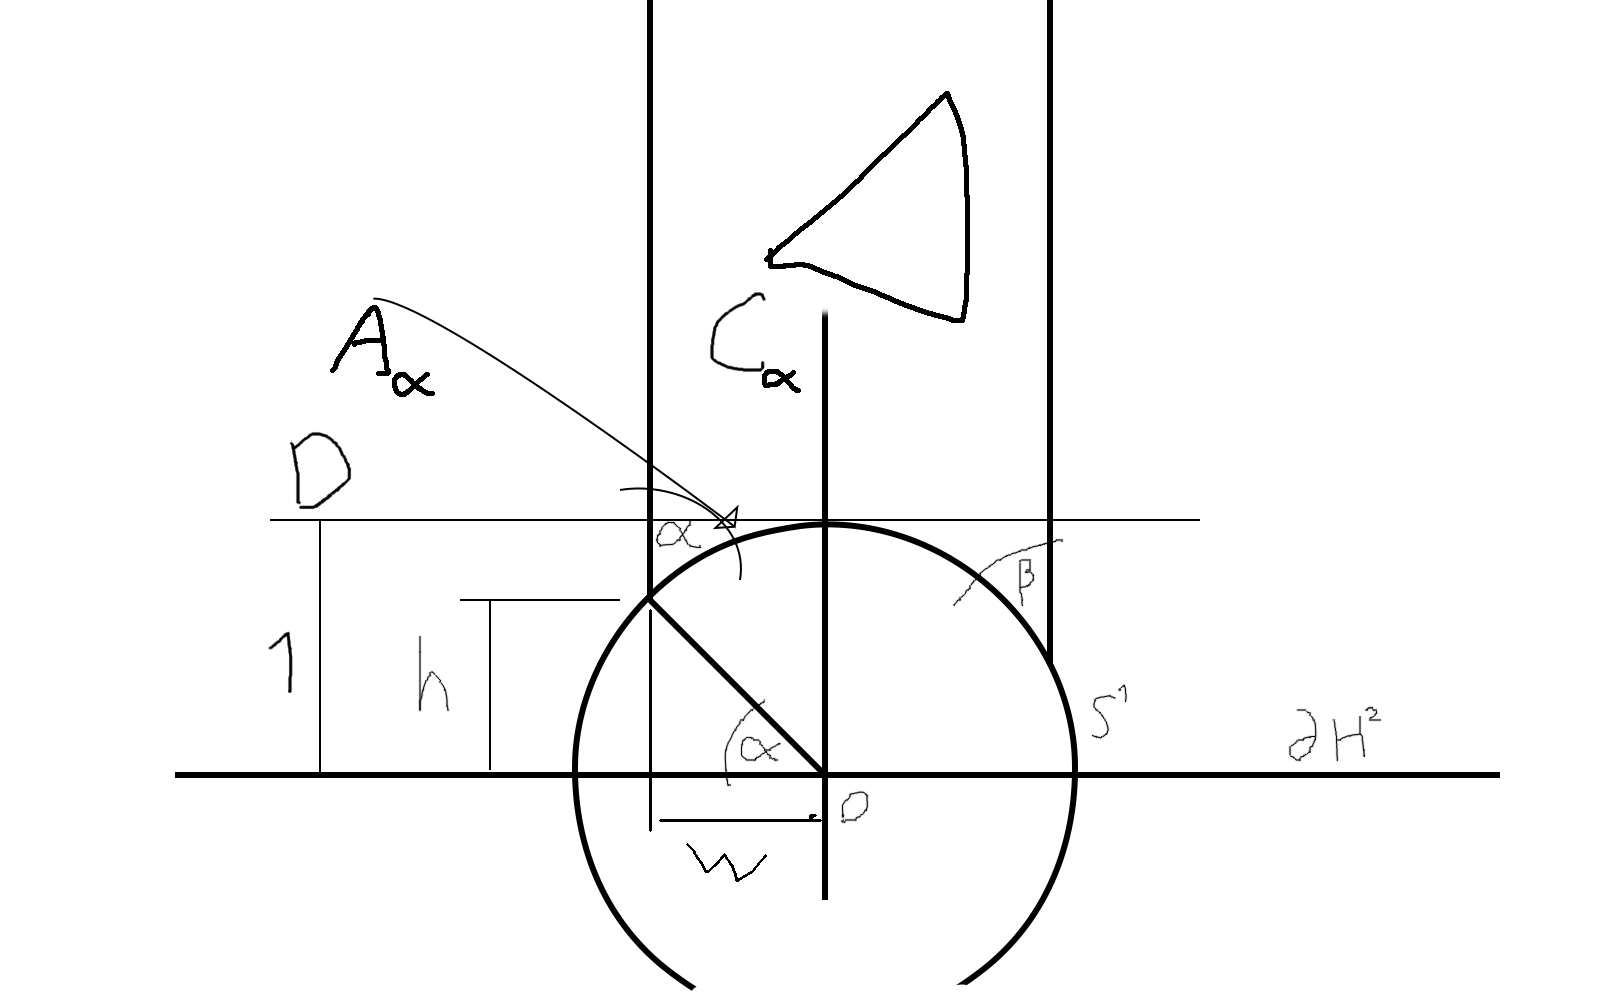
\includegraphics[scale = 0.3]{Skizze1.png}	
		\end{center}
		Wir können die Fläche von $\Delta$ also unterteilen in die Flächen von $A_{\alpha}, C_{\alpha}, A_{\beta}, C_{\beta}$. Die horizontale Linie $D$ der Höhe 1 bildet eine Horosphäre auf der die Metrik durch das euklidische Skalarprodukt gegeben ist. Insofern berechnet sich die Fläche von $C_{\alpha}$ durch
		\[ area(C_{\alpha}) = w = \cos(\alpha) \]
		Die Fläche von $A_{\alpha}$ berechnet sich durch das Integral
		\[ area(A_\alpha) = \int_{(x,y) \in A_{\alpha}}\frac{1}{y^2} \d x \d y = \int_{y = h}^{y = 1} \int_{x = -\cos(\sin\i(y))}^{x = -w} \frac{1}{y^2} \d x \d y \]
		wobei wir zuerst annehmen, dass $\alpha \neq 0$. Mit $h = \sin(\alpha), w = \cos(\alpha)$ berechnen wir
		\begin{align*}
		area(A_\alpha)  &= \int_{y = \sin \alpha}^{y = 1} \int_{x = -\cos(\sin\i(y))}^{x = -\cos \alpha} \frac{1}{y^2} \d x \d y \\
		&= \int_{y = \sin \alpha}^{y = 1} \frac{1}{y^2}\int_{x = -\cos(\sin\i(y))}^{x = -\cos \alpha}  \d x \d y \\
		&= -\int_{y = \sin \alpha}^{y = 1} \frac{\cos(\alpha) - \cos(\sin\i (y))}{y^2} \d y
		\end{align*}
		Wir substituieren $\sin u = y$
		\begin{align*}
		area(A_\alpha) &= -\int_{u = \alpha}^{u = \pi / 2} \frac{\cos(\alpha) - \cos(u)}{\sin(u)^2}\cos(u) \d u\\
		&= -\int_{u = \alpha}^{u = \pi / 2} \frac{\cos(\alpha)}{\sin(u)^2}\cos(u) \d u - \int_{u = \alpha}^{u = \pi / 2} \frac{ \cos(u)}{\sin(u)^2}\cos(u) \d u\\
		&\gl{(\ast)} -\cos(\alpha) [-\frac{1}{\sin(u)}]_{u = \alpha}^{u = \pi / 2} + [- u -\cot(u)]_{u = \alpha}^{u = \pi / 2}\\
		&= -\cos(\alpha)( - \frac{1}{\sin(\alpha)} + 1 ) + (-\alpha - \frac{\cos(\alpha)}{\sin (\alpha)} + \frac{\pi}{2})\\
		&= -\cos(\alpha) - \alpha +\frac{\pi}{2}
		\end{align*}
		Gleichung $(\ast)$ folgt aus Wolfram Alpha. Dieses Ergebnis für $A_\alpha$ ist aus Stetigkeitsgründen nun auch für den Fall $\alpha = 0$ anwendbar.\\
		Wir erhalten nun
		\begin{align*}
		area(\Delta) &= area(A_\alpha) + area(A_\beta)+ area(C_\alpha) + area(C_\beta) \\
		&= -\cos(\alpha) - \alpha +\frac{\pi}{2} -\cos(\beta) - \beta +\frac{\pi}{2} + \cos(\alpha)+\cos(\beta) \\
		&= \pi - \alpha - \beta
		\end{align*}
		
		\item[(ii)] Es liege nun keiner der Punkte bei Unendlich. Durch Isometrien lässt sich $\Delta$ so verschieben, dass die Seite $a$ in der imaginären Achse enthalten ist. Ohne Beschränkung der Allgemeinheit können wir also annehmen, dass folgende Situation vorliegt
		\begin{center}
			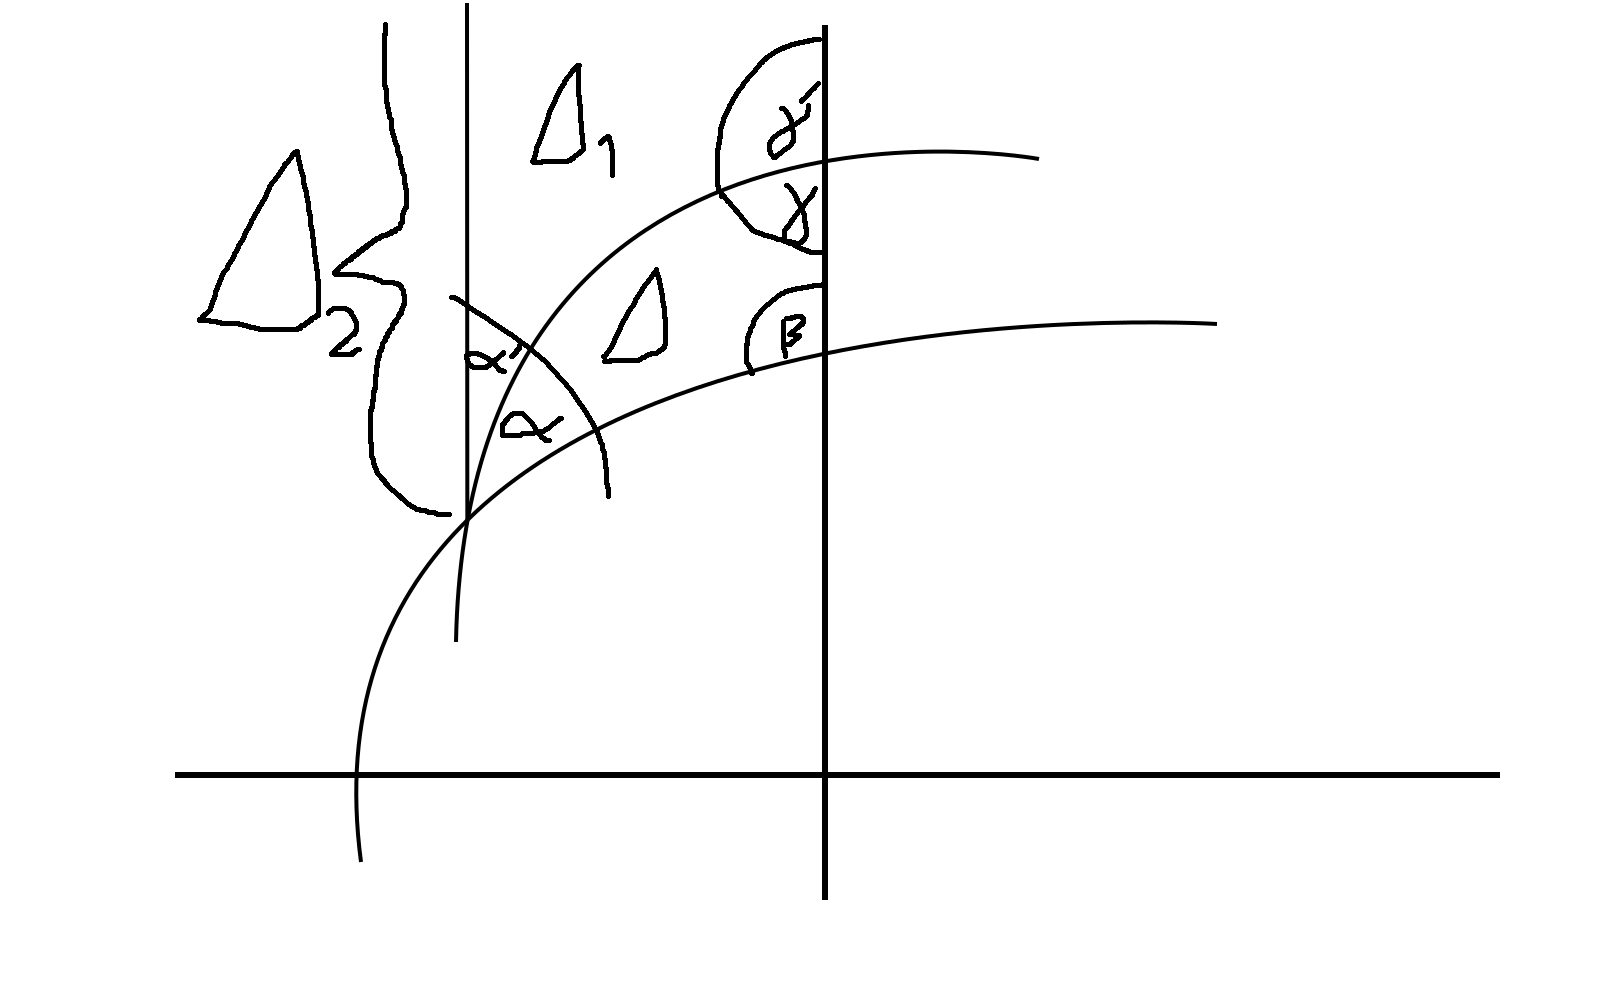
\includegraphics[scale = 0.3]{Skizze2.png}	
		\end{center}
		Die Flächeninhalte von $\Delta_1$ und $\Delta_2$ können wir dank des ersten Falls bestimmen. Es folgt nun
		\[ area(\Delta) = area(\Delta_2) - area(\Delta_1) = \pi - (\alpha + \alpha') - \beta - (\pi - \alpha' - \gamma') = \pi - \alpha - \beta - \gamma \]
	\end{enumerate}
\end{Beweis}

\subsubsection{Teilaufgabe 2}
\paragraph{Behauptung}
Ein hyperbolisches Polygon mit Inneren Winkeln $\alpha_1,\ldots, \alpha_n$ hat eine Flächenmaß von
\[ area(P) = (n-2)\pi - \sum_{i = 1}^{n} \alpha_i \]
\begin{Beweis}{}
	Sei $x$ ein innerer Punkt von $P$. Wir triangulieren $P$ anhand $x$ und erhalten $n$ Dreiecke $\Delta_1, \ldots, \Delta_n$. $\Delta_i$ hat dabei die Winkel $\beta_i, \gamma_i, \delta_i$ mit den Eigenschaften
	\begin{align*}
	\beta_i + \gamma_{(i\mod n)+1 } = \alpha_i \text{ für }i = 1,\ldots, n\\
	\delta_1 + \ldots + \delta_n = 2\pi
	\end{align*}
	Wir erhalten nun 
	\[ area(P) = \sum_{i = 1}^{n} area(\Delta_i) = \sum_{i = 1}^{n}(\pi - \beta_i - \gamma_i - \delta_i) = (n-2)\pi - \sum_{i = 1}^{n}\alpha_i \]
\end{Beweis}

\subsection{Aufgabe 2}
\subsubsection{Teilaufgabe 1}
Es bezeichne $\Gamma$ die Menge aller ganzzahligen 2x2-Matrizen mit Determinante 1, deren Inverses existiert und ebenfalls ganzzahlig ist.
\paragraph{Behauptung}
$\Gamma$ wird erzeugt durch
\begin{align*}
S =
\left(\begin{matrix}
0 & -1 \\
1 & 0
\end{matrix}\right)
\text{ und }
T  =
\left(\begin{matrix}
1 & 1 \\
0 & 1
\end{matrix}\right)
\end{align*}
\begin{Beweis}{}
	\begin{enumerate}[1.]
		\item Es gilt für $n \in \Z$
		\[ T^n = \left(\begin{matrix}
		1 & n \\
		0 & 1
		\end{matrix}\right) \]
		\item Ferner
		\[ S \cdot \left(\begin{matrix}
		a & b\\
		c & d
		\end{matrix}\right) = \left(\begin{matrix}
		-c & -d\\
		a & b
		\end{matrix}\right)
		\text{ und }
		\left(\begin{matrix}
		a & b\\
		c & d
		\end{matrix}\right)\cdot S   = \left(\begin{matrix}
		b & -a\\
		d & -c
		\end{matrix}\right)\]
		Mithilfe der Matrix $S$ können ergo Einträge bis auf einen Vorzeichenwechsel permutiert werden.
		\item Sei $A = \left(\begin{matrix}
		a & b\\
		c & d
		\end{matrix}\right) \in \Gamma$. Wir zeigen durch Vollständige Induktion nach $n = \bet{a} + \bet{d}$, dass $A$ durch $S$ und $T$ erzeugt wird.
		\begin{enumerate}
			\item[I.A.] $n = 0$.\\
			In diesem Fall sind $a = d = 0$ und $b,c\in \{\pm 1\}$, sodass $bc = -1$. Ergo ist $A$ entweder $S$ oder $S^3$.
			\item[I.S.] $n>0$ ist beliebig, aber fest.\\
			Wir können ohne Beschränkung der Allgemeinheit annehmen, dass $a,b,c,d > 0$ und $a > d$. Da $ad -bc = 1$, folgt dann insbesondere auch $a>b,c$. Betrachte nun
			\[ T\i A \cdot T\i = \left(\begin{matrix}
			a - c - b +d & b - d\\
			c - d & d
			\end{matrix}\right)\]
		Wir behaupten, dass
		\[ \bet{ a + d -b -c }< a \]
		Angenommen, dem wäre nicht so. In jedem Fall muss $a + d > b +c$ gelten, da sonst die Determinante nicht Eins wäre. Es folgt aus der Annahme
		\[ d\geq b+c \]
		Aber dann gilt
		\[ ad -cb\geq ab + ac -cb\geq ab > 1 \]
		Was ein Widerspruch ist. Ergo können wir durch das beidseitige Ranmultiplizieren von $T\i$ erreichen, dass $\bet{a} + \bet{d}$ kleiner wird. Der Rest folgt nun aus der Induktionsvoraussetzung.
		\end{enumerate}
	\end{enumerate}
\end{Beweis}

\subsubsection{Teilaufgabe 2}
\paragraph{Behauptung}
$\Gamma$ wirkt eigentlich diskontinuierlich, aber nicht frei auf $H^2$.
\begin{Beweis}{}
	Die Wirkung ist nicht frei, da
	\[ i.S = \frac{-1}{i} = i \]
	Nichtsdestotrotz ist sie eigentlich diskontinuierlich. Denn sei $K \subset H^2$ kompakt. Dann ist die Menge
	\[ A = \set{g \in PSL_2(\R)}{K.g \cap K \neq \emptyset} \]
	kompakt in $PSL_2(\R)$. Da $\Gamma$ diskret in $PSL_2(\R)$ liegt, muss
	\[ \set{g \in PSL_2(\Z)}{K.g \cap K \neq \emptyset} = \Gamma \cap A \]
	endlich sein.
\end{Beweis}

\subsubsection{Teilaufgabe 3}
Definiere das hyperbolische Dreieck $D$ durch
\[ D:= \set{z \in H^2}{ \bet{Re(z)} \leq \frac{1}{2}, \bet{z} \geq 1 } \]
\paragraph{Behauptung}
$D$ ist ein Fundamentalbereich von $\Gamma$.
%\begin{Beweis}{}
%	Setze $S = \set{2i.\gamma}{\gamma \in \Gamma}$. Dann bilden die Mengen
%	\[ D(s) = \set{ p \in H^2}{d(s,p) \leq d(q,p) \forall q \in S} \]
%	für $s \in S$ eine Kachelung von $H^2$. Es bleibt zu zeigen, dass $D = D(2i)$.
%\end{Beweis}

\subsubsection{Teilaufgabe 4}
\paragraph{Behauptung}
\[ area(D) = \frac{\pi}{3} \]
\begin{Beweis}{}
	$D$ wird gerade durch ein Dreieck mit Eckpunkten $-\frac{\sqrt{3}}{2},  \frac{\sqrt{3}}{2}, \infty$ beschränkt. Die inneren Winkel dieses Dreiecks betragen $\frac{\pi}{3},\frac{\pi}{3}$ und Null. Aus Aufgabe 1 folgt nun, dass $D$ eine Fläche von $\frac{\pi}{3}$ hat.
\end{Beweis}

%\newpage
\subsection{Aufgabe 3}
Sei $\Delta \subset H^2$ ein Dreieck, dessen Fläche echt zwischen 0 und $\pi$ liegt und das Winkel $\frac{\pi}{a}, \frac{\pi}{b}, \frac{\pi}{c}$ für natürliche Zahlen $a,b,c$ hat. Bezeichne mit $\Gamma$ die Gruppe, die durch die Spiegelungen entlang den Seiten von $\Delta$ erzeugt wird.
\subsubsection{Teilaufgabe 1}
\paragraph{Behauptung}
$\Gamma$ wirkt auf $H^2$ eigentlich diskontinuierlich, aber nicht frei.
\begin{Beweis}{}
	$\Gamma$ wirkt tatsächlich nicht frei, denn liegt $x$ auf einer Seite von $\Delta$ und bezeichnet $\phi$ die Spiegelung an dieser Seite, so gilt $\phi(x) = \phi$, obwohl $\phi$ nicht trivial ist.\\
	Es genügt nun zu zeigen, dass $\Gamma$ diskret in $Isom(H^2)$ liegt.\\
Man sieht, dass $\set{g(\Delta)}{g \in \Gamma}$ eine Kachelung von $H^2$ liefert. Insbesondere besitzt jeder Punkt $x\in H^2$ eine Umgebung, die nur endlich viele dieser Kacheln schneidet. Ergo agiert $\Gamma$ eigentlich diskontinuierlich.
\end{Beweis}
\subsubsection{Teilaufgabe 2}
\paragraph{Behauptung}
$\Delta$ ist gerade ein Fundamentalbereich für $\Gamma$.


\subsection{Aufgabe 4}
\subsubsection{Teilaufgabe 1}
\paragraph{Behauptung}
Jede geschlossene, flache, orientierbare Fläche ist ein Torus.
%\begin{Beweis}{}
%	Sei $C$ eine geschlossene, flache, orientierbare Fläche. Da eine Fläche Sein vermutlich geodätisch vollständig impliziert, können wir annehmen, dass $C$ durch den $\R^2$ überlagert wird und durch das Herausteilen einer isometrischen, eigentlich diskontinuierlichen Wirkung $\Gamma \subset Isom(\R^2)$ induziert wird.\\
%	Da $C$ geschlossen ist, gibt es eine nichttriviale sphärische Geodäte $\gamma : S^1 \pfeil{} C$. Diese lässt sich liften zu einer Geodäten $\gamma' : \R^1 \pfeil{} \R^2$. Ferner gibt es ein nichttriviales Element $\alpha \in \Gamma$, dass $\gamma'$ invariant lässt, d.\,h., $\alpha(\gamma(\R)) = \gamma(\R)$. $\alpha$ besitzt die Gestalt
%	\[ \alpha(x) = Ax + b \]
%	für $A \in O(2), b \in \R^2$. Am Punkt $\gamma(0)$ sei eine Basis des Tangentialraums durch $\gamma'(0)$ und einen orthogonalen Vektor $v$ gegeben. Da $\gamma$ stabil unter $\alpha$ ist, gilt
%	\[ A\gamma'(0) = \gamma'(0) \]
%	Da $A \in O(2)$, folgt damit
%	\[ Av = zv \]
%	für $z = \pm 1$. Da $C$ orientierbar ist, muss $A$ orientierungserhaltend sein, es folgt $z = 1$, d.\,h., $A = E_2$. Es folgt
%	\[ \alpha(x) = x + b \]
%	für $b \in \R^2\setminus \{0\}$.\\
%	Es bezeichne $\Gamma_\alpha$ die Untergruppe, die durch $\alpha$ erzeugt wird. Teilt man diese raus, erhält man folgende Sequenz von Überlagerungen
%	\[ \R^2 \Pfeil{} \R^2 / \Gamma_\alpha \Pfeil{} C \]
%	$\R^2 / \Gamma_\alpha$ ist dabei seinerseits ein flacher Zylinder, also nicht abgeschlossen.\\
%	Sei $\beta'$ eine Geodäte in $\R^2$, die orthogonal zu $\gamma$ verläuft. Wir erhalten hierdurch eine unendliche Geodäte $\beta$ in $\R^2 / \Gamma_\alpha$, die orthogonal zur Nabe des Zylinders steht. Bezeichne $\Gamma'$ die Decktransformationsgruppe von $\R^2 / \Gamma_\alpha \surj{} C$. Die Decktransformationen von $\R^2 / \Gamma_\alpha \surj{} C$ können die Ausrichtung der Nabe des Zylinders nicht ändern, da sie abstands- und orientierungserhaltend sind. Ergo wird $\beta$ unter $\Gamma'$ auf andere unendliche Geodäten abgebildet, die orthogonal zur Nabe sind. Es bezeichne $\beta.\Gamma'$ den Orbit von $\beta$. Dieser ist enthalten in einer kompakten Menge, die diffeomorph zu $S^1$ ist. Da $\Gamma'$ eigentlich diskontinuierlich wirkt, ist der Orbit von $\beta$ endlich.\\
%	Da $C$ geschlossen ist, muss es ein Element in $\delta \in \Gamma'$ geben, welches die Nabe des Zylinders verschiebt. Insbesondere dreht $\delta$ die Geodäte $\beta$ um die Achse des Zylinders. Da der Orbit von $\beta$ endlich ist, gibt es ein $n \in \N$, sodass $\delta^n$ die Geodäte $\beta$ fixiert, aber nichttrivial ist. Teilt man die Wirkung der Gruppe, die durch $\delta^n$ erzeugt heraus, so erhält man einen Torus $T$, welcher weiterhin $C$ überlagert. Es ergeben sich folgende Überlagerungen
%	\[ \R^2 \Pfeil{} \R^2 / \Gamma_\alpha \Pfeil{} T \Pfeil{} C \]
%	Die orientierungserhaltenden Isometrien des Torus sind ausschließlich Drehungen und Verschiebungen der Nabe. Teilt man ergo die Decktransformationsgruppe von $T \surj{} C$ aus $T$ raus, so ergibt sich wieder ein Torus. Ergo folgt die Behauptung.
%\end{Beweis}
\begin{Beweis}{}
	Sei $C$ eine geschlossene, flache, orientierbare Fläche. Da $C$ eine geschlossene Fläche ist, können wir annehmen, dass $C$ durch den $\R^2$ überlagert wird und durch das Herausteilen einer isometrischen, eigentlich diskontinuierlichen, freien und orientierungserhaltenden Wirkung $\Gamma \subset Isom(\R^2)$ induziert wird.\\
	Ein nichttriviales Element $\gamma \in \Gamma$ wirkt nun durch
	\[ x \mapsto Ax + b \]
	für $x \in \R^2, b\in \R^2, A \in O(2)$ mit $\det A = 1$.\\
	$A$ muss nun aber die Einheitsmatrix sein, da sich sonst folgendes LGS
	\[ Ax + b = x \Gdw{} (A - I)x = b \]
	lösen lässt und $\gamma$ einen Fixpunkt hätte. Nun ist aber $\Gamma$ offensichtlich ein Gitter in $\R^2$ der Dimension $\leq 2$. $C$ ist genau dann geschlossen, wenn $\Gamma$ Dimension 2 hat und deswegen einen Torus induziert.
\end{Beweis}


\subsubsection{Teilaufgabe 2}
\paragraph{Behauptung}
Die Kleinsche Flasche ist eine geschlossene flache Fläche, die nicht orientierbar ist.
\begin{Beweis}{}
	Die Kleinsche Flasche wird durch den $\R^2$ überlagert und besitzt ohne Beschränkung der Allgemeinheit folgenden Fundamentalbereich.
	\begin{center}
		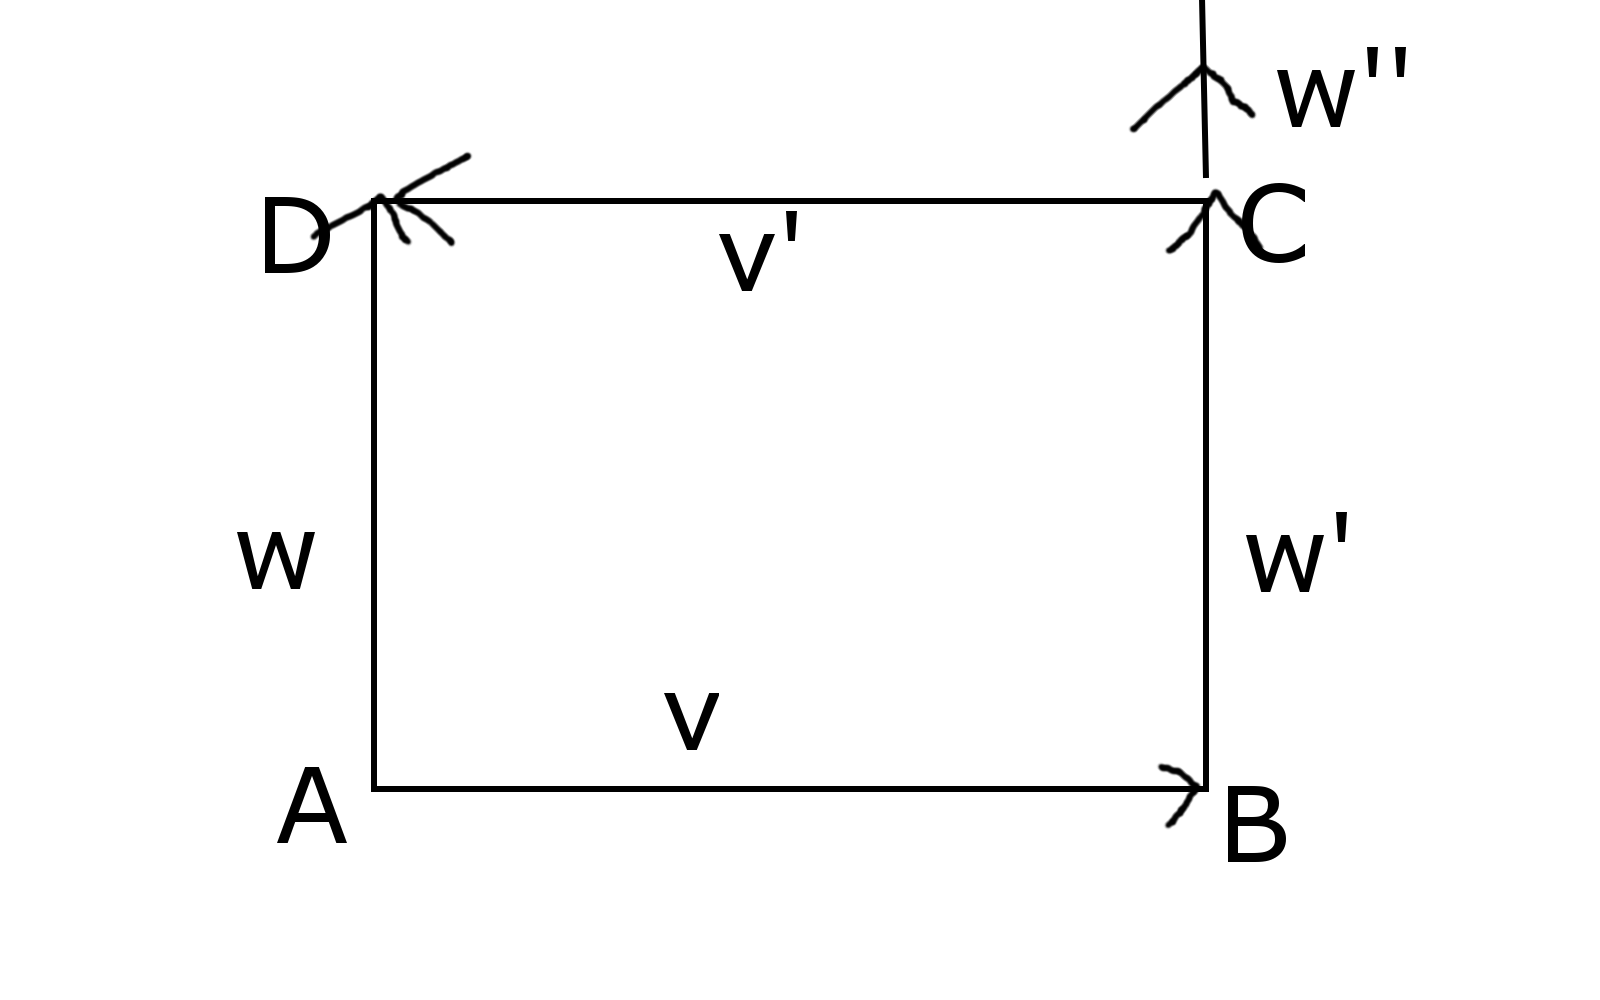
\includegraphics[scale = 0.15]{Skizze3.png}	
	\end{center}
	Insofern folgt bereits, dass die Kleinsche Flasche geschlossen und flach ist. Da die Punkte $A,B,C,D$ und die Seiten $v,v'$ und $w,w'$ unter der Decktransformationsgruppe $\Gamma$ jeweils identifiziert werden, gibt es eine Decktransformation $\gamma \in \Gamma$ mit
	\[ \gamma(A) = C, \d \gamma(v) = v', \d\gamma(w) = w'' \]
	Aber daraus folgt sofort, dass $\gamma$ nicht orientierungserhaltend ist, d.\,h., $\det \d\gamma = -1$. Ergo ist die Kleinsche Flasche nicht orientierbar.
\end{Beweis}

\subsubsection{Teilaufgabe 3}
\paragraph{Behauptung}
Jede Überlagerung der Kleinschen Flasche durch den Torus hat einen geraden Grad.
\begin{Beweis}{}
	Bezeichnet $T$ den Torus und $K$ die kleinsche Flasche, so erhält man für gerades $n$ eine Überlagerung $T\surj{}K$ durch eine Isometrie $\phi_n$, die $T$ um $\frac{2\pi}{n}$ um seine Achse dreht und die Orientierung der Nabe von $T$ umdreht.\\
	Ist eine Überlagerung $\varphi : T \surj{} K$ gegeben, so können wir die Wirkung von $\varphi$ auf dem Fundamentalbereich betrachten, die in etwa wie folgt aussieht
	\begin{center}
		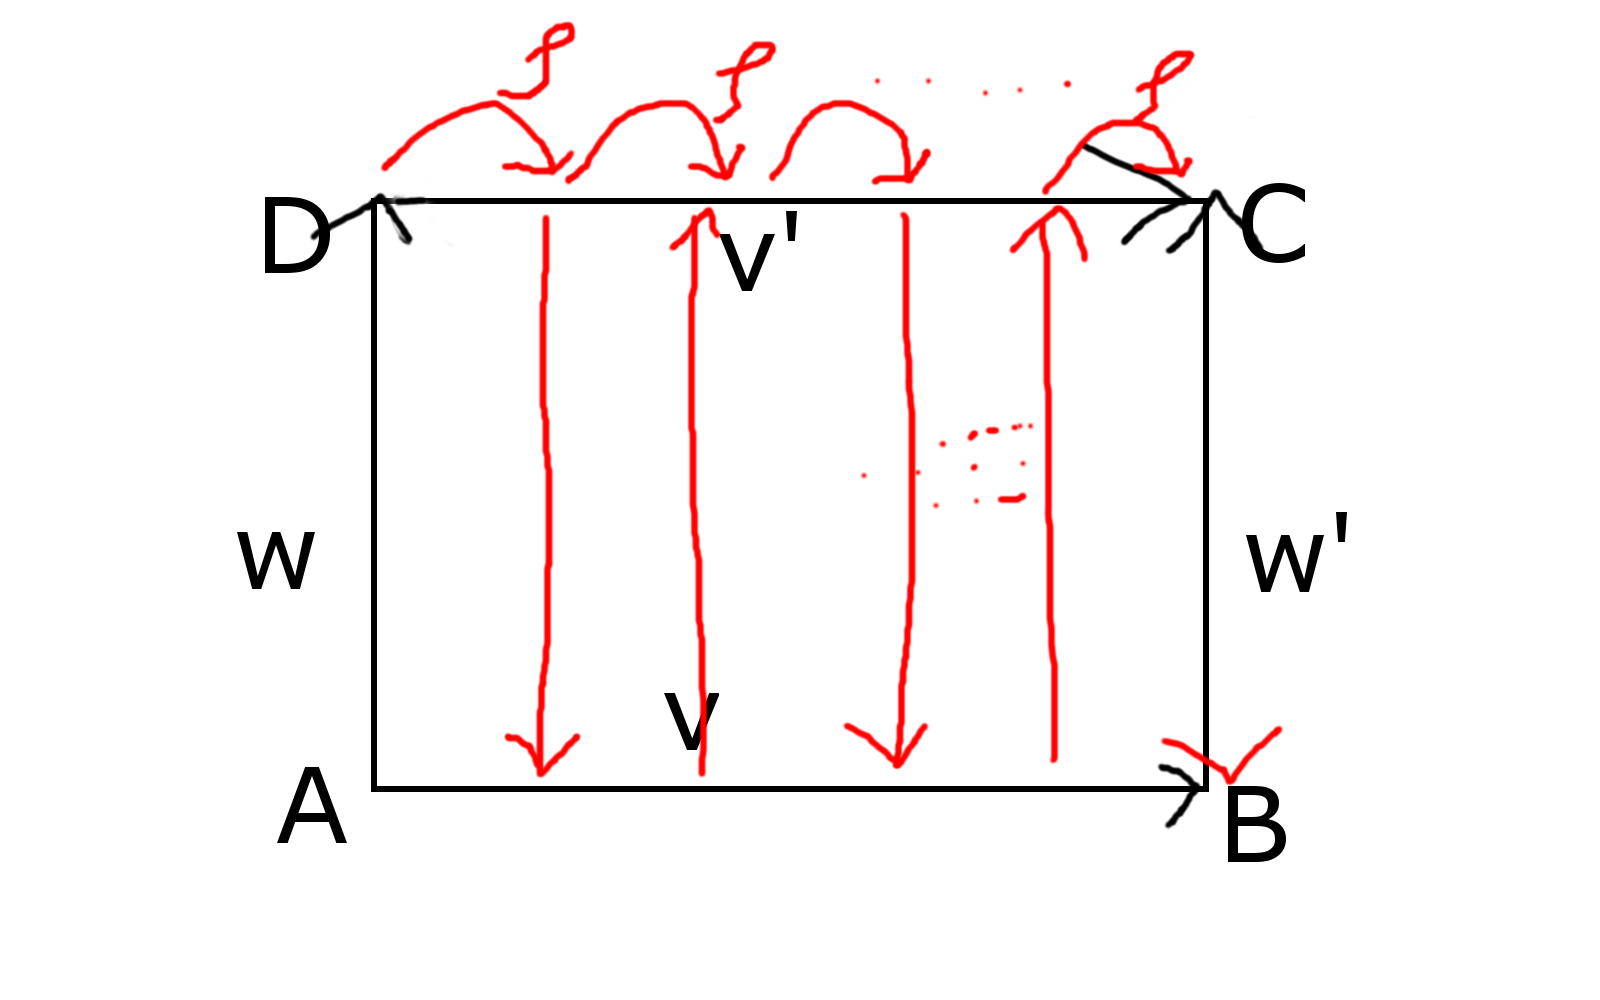
\includegraphics[scale = 0.15]{Skizze4.png}	
	\end{center}
	Damit $\varphi$ die Orientierung tatsächlich umkehrt, muss $\varphi$ eine gerade Ordnung haben, daraus resultiert ein gerader Grad der Überlagerung.
\end{Beweis}

\subsection{Aufgabe 5}
Sei $M = S^n / \Gamma$ eine elliptische Mannigfaltigkeit, wobei $\Gamma$ frei und eigentlich diskontinuierlich wirkt, und $n$ gerade.
\paragraph{Behauptung}
Es ist $M = S^n$ oder $M = P\R^n$.
\begin{Beweis}{}
	Es gilt
	\[ Isom(S^n) = O(n+1) \]
	Sei $A \in O(n+1)$ von Determinante $+1$. Dann besitzt $A$ mindestens einen Fixpunkt. Denn sind $\lambda_1, \ldots, \lambda_k\in \{\pm 1\}$ die reellen Eigenwerte von $A$ und $\lambda_{k+1},\ldots,\lambda_{n+1}\in S^1$ die komplexen Eigenwerte, so gilt
	\begin{align*}
	\prod_{i = 1}^{n+1} \lambda_i & = 1\\
	k &\text{ ist ungerade}\\
	\lambda_{k+1 + 2i} &= \overline{ \lambda_{k+2 + 2i}} \text{ für }i\geq 0
	\end{align*}
	Ergo muss mindestens einer der Eigenwerte von $A$ +1 sein.\\
	Ist nun $A \in O(n+1)$ nicht selbstinvers, so besitzt $A^2$ Determinante 1 und somit einen Fixpunkt, und kann ergo nicht in $\Gamma$ liegen. Die Elemente in $\Gamma$ sind ergo selbstinvers. Für selbstinverse Elemente $A \in O(n+1)$ gilt
	\[ A = A\i = A^T \]
	Ergo ist $A$ symmetrisch und orthogonal. Die symmetrischen und orthogonalen Matrizen sind aber genau die, die Diagonalmatrizen mit Diagonaleinträgen $\pm 1$ sind. Besitzt $A$ sowohl $+1$ als auch $-1$ als Diagonaleintrag, so ist $A$ weder trivial noch fixpunktfrei. Ergo kann $\Gamma$ nur $E_n$ und $-E_n$ besitzt.\\
	Ist $\Gamma = \{E_n\}$, so folgt $M = S^n$. Ansonsten ist $\Gamma = \{\pm E_n \}$ und $M = P\R^n$. 
\end{Beweis}

\subsection{Aufgabe 6}
Seien $p,q>1$ teilerfremd und $\theta := e^{\frac{2\pi i}{p}}$. Definiere auf $S^3 \subset \C^2$ die Abbildung
\[ f(z_1,z_2) := (\theta z_1, \theta^q z_2) \]
Es bezeichne $\Gamma$ die Gruppe, die durch $f$ erzeugt wird.
\subsubsection{Teilaufgabe 1}
\paragraph{Behauptung} $f$ ist eine Isometrie.
\begin{Beweis}{}
	Seien $(z_1,z_2), (w_1,w_2) \in S^3$. Wir rechnen nach
	\begin{align*}
	d(f(z_1,z_2), f(w_1,w_2))^2 &= d( (\theta z_1, \theta^p z_2) , (\theta w_1, \theta^p w_2) )^2\\
	&= \bet{ \theta z_1 - \theta w_1 }^2 + \bet{\theta^p z_2 - \theta^p w_2 }^2 \\
	&= \bet{z_1 - w_1}^2 + \bet{z_2 - w_2}^2 = d((z_1,z_2), (w_1, w_2))
	\end{align*}
	da $\bet{\theta} = 1$. Ergo ist $f$ eine abstandserhaltende Selbstabbildung und dadurch, da $S^3$ zusammenhängend ist, eine Isometrie.
\end{Beweis}

\subsubsection{Teilaufgabe 2}
\paragraph{Behauptung} Der \df{Linsenraum}
$L(p,q) := S^3 / \Gamma$
ist eine elliptische Mannigfaltigkeit.

\begin{Beweis}{}
	Es genügt zu zeigen, dass $\Gamma$ frei und eigentlich diskontinuierlich auf $S^3$ wirkt. Beachte hierbei, dass die Ordnung von $f$ genau $p$ ist.\\
	Sei also $(z,w) \in S^3$ und $n \in \N$, sodass $f^n(z,w) = (z,w)$. Es gilt
	\[ f^n(z,w) = (\theta^nz, \theta^{nq}w) = (e^{2\pi i\frac{n}{p}}z, e^2{2\pi i \frac{nq}{p}}w) = (z,w) \]
	Dies ist genau dann der Fall, wenn
	\[ \frac{n}{p}, \frac{nq}{p} \in \Z \]
	was wiederum genau dann der Fall ist, wenn $p|n$ und $p|nq$, also wenn $n$ ein Vielfaches der Ordnung von $f$ ist. Ergo besitzt nur das triviale Element in $\Gamma$ einen Fixpunkt.\\
	Da die Ordnung von $f$ endlich ist, ist $\Gamma$ endlich und liegt somit diskret in $Isom(S^3)$. Ergo agiert $\Gamma$ deswegen eigentlich diskontinuierlich.
\end{Beweis}

\newpage
\section{Blatt 3}
\subsection{Aufgabe 2}
Sei $M = \H^n / \Gamma$ eine vollständige, hyperbolische Mannigfaltigkeit. $[S^1, M]$ bezeichne die Menge der Homotopieklassen stetiger Abbildungen des Typs $S^1 \pfeil{} M$.
\subsubsection{Teilaufgabe 1}
\paragraph{Behauptung} Sei $x_0 \in M$ beliebig. Dann ist die Abbildung
\begin{align*}
\Phi : \pi_1(M,x_0) & \Pfeil{} [S^1, M]\\
[\gamma] & \longmapsto [\gamma]
\end{align*}
wohldefiniert und surjektiv. Für zwei Elemente $\gamma,\sigma \in \pi_1(M,x_0)$ gilt
\[ \Phi(\gamma) = \Phi(\sigma) \Gdw{} \gamma \text{ und }\sigma  \text{ sind konjugiert}\]
\begin{Beweis}{}
	Die Abbildung ist offensichtlich wohldefiniert. Da $M$ zusammenhängend ist, ist sie auch offensichtlich surjektiv.\\
	Seien $f,g \in \in \pi_1(M,x_0)$ mit $\Phi(f) = \Phi(g)$. Dann existiert eine (nicht Endpunkt erhaltende) Homotopie $H : I \times S^1 \pfeil{} M$ mit
	\[ H_0 = f \text{ und } H_1 = g \]
	Da die Endpunkte von $f$ und $g$ gerade $x_0$ sind, gilt $H_t(1) = H_t(0)$. Insbesondere liefert $H_t(1) =:c$ eine Schleife von und zu $x_0$. Es folgt nun aufgrund des Homotopiequadrates
	\[ c f = gc \]
	Sind umgekehrt $f$ und $g$ durch ein $c$ wie oben konjugiert, so existiert eine Homotopie $cf \sim gc$ in $\pi_1(M,x_0)$. Dies liefert eine Homotopie $f\sim g$ in $[S^1, M]$.
\end{Beweis}

\subsubsection{Teilaufgabe 2}
\paragraph{Behauptung} Die Konjugationsklassen hyperbolischer Elemente $\gamma \in \Gamma$ stehen in Eins-zu-Eins-Korrespondenz zu geschlossenen Geodäten von $c\subset M$. Insbesondere gilt
\[ l(c) = d(\gamma) \]
\begin{Beweis}{}
	Sei $l$ die geodätische Achse von $\gamma$. Dann wird $l$ in $M$ auf eine geschlossene Geodäte abgebildet, deren Länge der Versetzung von $\gamma$ entspricht. Sei nun $\sigma$ konjugiert zu $\gamma$. Beide korrespondieren zu Schleifen in $\pi_1(M, x_0)$ und werden auf dasselbe Element in $[S^1, M]$ abgebildet. Ergo sind die geschlossenen Geodäten, die sie induzieren, homotop zueinander und müssen deswegen übereinstimmen.
\end{Beweis}

\subsubsection{Teilaufgabe 3}
\paragraph{Behauptung}
Jede geschlossene Geodäte hat minimale Länge in seiner Homotopieklasse.
\begin{Beweis}{}
	Sei $\gamma$ eine geschlossene Geodäte und $c$ homotop zu $\gamma$. Seien $\widetilde{c}$ und $\widetilde{\gamma}$ Hebungen mit denselben Endpunkten. Es gilt
	\[ l(c) \geq d(x,\phi(x)) \geq d(\phi) = l(\gamma) \]
\end{Beweis}

\subsection{Aufgabe 3}
Sei $M = \H^n / \Gamma$ eine Mannigfaltigkeit endlichen Volumens. Dann ist das Zentrum von $\Gamma$ in $Isom(\H^n)$ trivial.
\begin{Beweis}{}
	Sei $h \in Z(\Gamma)$ nichttrivial. Dann gilt für alle nichttriviale $\phi \in \Gamma$
	\[ Fix(\phi) = Fix(h) \]
	D.\,h., $\Gamma$ wird von einer Hyperbolischen erzeugt oder von mehreren Parabolischen, die denselben Punkt im Unendlichen fixieren. Im ersten Fall ist $M$ eine unendliche Tube, im zweiten Fall eine unbegrenzte Spitze. Beide Mannigfaltigkeiten haben kein endliches Volumen.
\end{Beweis}

\subsection{Aufgabe 4}
Sei $\H^n / \Gamma$ eine vollständige, hyperbolische Mannigfaltigkeit.
\subsubsection{Teilaufgabe 1}
\paragraph{Behauptung}
Jede Untergruppe von $\Gamma$, die isomorph zu $\Z^2$ ist, besteht aus Parabolischen, die denselben Punkt im Unendlichen fixieren.
\begin{Beweis}{}
	Sei $U \subset \Gamma$ mit $U \isom{} \Z^2$. Da $U$ abelsch und diskret ist, müssen alle Elemente in $U$ denselben Typ haben, denn, erstens, $U$ kann keine elliptischen Elemente haben, da $\Gamma$ frei wirkt und, zweitens, zwei Elemente in $U$ müssen nun dieselben Fixpunkte haben, da $U$ abelsch ist.\\
	$\phi_1,\phi_2$ bezeichne die beiden Erzeuger von $U$.\\
	Sind beides Hyperbolische, die dieselbe geodätische Achse fixieren, so muss es aus Diskretheitsgründen $l,k> 0$ geben mit 
	\[ \phi_1^l = \phi_2^k \]
	Dies stellt aber einen Widerspruch zur Unabhängigkeit der beiden Erzeuger dar.\\
	Ergo können $\phi_1, \phi_2$ nur noch Parabolische mit demselben Fixpunkt im Unendlichen sein. 
\end{Beweis}
\subsubsection{Teilaufgabe 2}
\paragraph{Behauptung}
Der $n$-Torus kann für $n\geq 2$ keine hyperbolische Struktur besitzen.
\begin{Beweis}{}
	Angenommen wir hätten $T^n = \H^n / \Gamma$. Dann gälte $\Gamma = \Z^n$. Folglich müsste $\Gamma$ Parabolische enthalten, die denselben Punkt im Unendlichen fixieren. Wir wissen aber, dass $\H^n / \Gamma$ genau dann kompakt ist, wenn $\Gamma$ nur aus Hyperbolischen besteht. Ein Widerspruch.
\end{Beweis}

\subsection{Aufgabe 5}
Sei $\H^n / \Gamma$ eine vollständige, hyperbolische Mannigfaltigkeit. Für $\phi \in \Gamma$ setze
\[S = S_\phi(\epsilon) := \set{x \in \H^n}{ d(\phi(x), x) \leq \epsilon } \] 
\paragraph{Behauptung}
Ist $\phi$ parabolisch mit Fixpunkt $p$, so ist $S$ eine sternförmige Umgebung um $p$. Ist $\phi$ hyperbolisch mit Achse $l$, so ist $S$ eine sternförmige Umgebung um $l$.
\begin{Beweis}{}
	\begin{itemize}
		\item Sei $\phi$ parabolisch mit Fixpunkt $p$. Sei $g \subset \H^n$ eine Geodäte, das einen Endpunkt in $p$ hat. Wir müssen zeigen, dass der Schnitt $g\cap S$ nichtleer und zusammenhängend ist. Tatsächlich ist der Schnitt
		\[ g\cap S = \set{ x \in g }{d(x, \phi(x))\leq \epsilon } \]
		nichtleer, da $d(x, \phi(x))$ gegen Null konvergiert, wenn $x$ auf $g$ entlang gegen $p$ konvergiert. Diese Menge ist auch zusammenhängend, denn $\phi(g)$ ist ebenfalls eine Geodäte, die gegen $p$ konvergiert. Wird $g$ durch $g(t)$ parametrisiert, so folgt aus $d(g(t_0), \phi(g(t_0))) \leq \epsilon$ ergo $d(g(t), \phi(g(t))) \leq \epsilon$ für alle $t\geq t_0$. Dies muss gelten, da $\phi$ jede Horosphäre um $p$ erhält.
		\item Sei $\phi$ hyperbolisch mit Achse $l$. Ist $\epsilon < d(\phi)$, so ist $S$ leer. Ist $\epsilon = d(\phi)$, so ist $S = l$ und somit keine Umgebung.\\
		Sei nun $\epsilon > d(\phi)$. Sei $g$ eine Geodäte, die $l$ orthogonal schneidet. Offensichtlich ist dann der Schnitt mit $S$ nicht-leer. Betrachte die Geodäte $\phi(g)$. $g$ und $\phi(g)$ sind ultra-parallel, ihr minimaler Abstand wird genau auf $l$ realisiert. Von $l$ weg, nimmt der Abstand zwischen beiden monoton zu. Ergo ist $S \cap g$ zusammenhängend.
	\end{itemize}
\end{Beweis}

\subsection{Aufgabe 6}
Sei $\Gamma \subset Isom(\H^n)$ diskret und nichttrivial.
\subsubsection{Teilaufgabe 1}
Die Limes-Menge
\[ \Lambda(\Gamma) = \overline{\Gamma.x} \cap \partial \H^n \]
ist unabhängig von der Wahl von $x \in \H^n$.
\begin{Beweis}{}
	Seien $x,y \in \H^n$. Sei $(g_i(x))_i$ eine Folge in $\Gamma.x$, die gegen einen Punkt $p \in \partial \H^n$ konvergiert. $x$ und $y$ haben einen endlichen Abstand und die Folgen $(g_i(x))$ und $g_i(y))$ haben gliedweise denselben endlichen Abstand. Ergo konvergieren sie gegen denselben Punkt im Unendlichen.
\end{Beweis}

\subsubsection{Teilaufgabe 2}
Ist $\Gamma' \subset \Gamma$ von endlichem Index, so gilt
\[ \Lambda(\Gamma') = \Lambda(\Gamma) \]
\begin{Beweis}{}
	Sei $(g_i(x))_i$ eine Folge in $\Gamma.x$, die gegen einen Punkt $p \in \partial \H^n$ konvergiert. Wir nehmen an, dass alle $g_i$ nicht in $\Gamma'$ liegen. Da $\Gamma / \Gamma'$ endlich ist, gibt es ein $h \in \Gamma$, sodass unendlich viele der $g_ih$ in $\Gamma'$ liegen. Ergo ist $p$ ein Häufungspunkt von $\Gamma'.h\i(x)$.
\end{Beweis}


\newpage
\section{Blatt 4}
\subsection{Aufgabe 1}
Seien $\gamma_1,\ldots, \gamma_n \in Isom(D^n)$ hyperbolisch. $D_1,\ldots, D_n$ seien offene Mengen mit
\begin{itemize}
	\item $D_i \cap g(D_i) = \emptyset ~~~\forall g = \gamma_i^k, k \in \Z \setminus\{0\}$
	\item $ D:= \bigcap_{i = 1}^n D_i \neq \emptyset $
	\item $D_i \cup D_j =D^n~~~\forall i \neq j$ 
\end{itemize}
\subsubsection{Teilaufgabe 1 und 2}
\paragraph{Behauptung}
$\Gamma:= \shrp{\gamma_1,\ldots, \gamma_n}$ ist das Koprodukt der $\shrp{\gamma_i}$ in der Kategorie der Gruppen, oder anders ausgedrückt, $\Gamma$ wird frei von den $\gamma_i$ erzeugt.\\
Ferner gilt für alle $g \in \Gamma, g\neq 1,$
\[ D \cap g(D) = \emptyset \]
\begin{Beweis}{}
	Wir zeigen, dass es keine nichttrivialen Relationen in $\Gamma$ gibt. D.\,h., ist $1 = g_1\ldots g_k$ mit $g_j \in \shrp{\gamma_{i_j}}$ und $i_j \neq i_{j+1}$, so muss eines der $g_i$ trivial sein.\\
	Wir führen dazu eine vollständige Induktion nach $k$ durch. Der Induktionsanfang ist klar.\\
	Sei die Aussage für $k$ bewiesen und $g_1 \ldots g_{k+1} = 1$ in $\Gamma$. Da $g_{k+1} \neq 1$, gilt
	\[ g_{k+1}(D_{i_{k+1}}) \subset D_{i_{k+1}}^C \subset D_{i_k} \]
	und somit
	\[ g_1\ldots g_{k+1} (D_{i_{k+1}}) \subset D_{i_1}^C  \]
	und insbesondere
	\[ g_1\ldots g_{k+1} (D) \subset D^C  \]
	ergo gilt $ g_1\ldots g_{k+1}\neq 1$.
\end{Beweis}

\subsubsection{Teilaufgabe 3}
\paragraph{Behauptung}
$\Gamma$ ist diskret.
\begin{Beweis}{}
	Sei $g_n$ eine Folge in $\Gamma$, die gegen die Identität konvergiert. Für alle $g_n \neq 1$ gilt
	\[ g_n(D) \cap D = \emptyset \]
	Aus Stetigkeitsgründen gibt es ein $N$, sodass für alle $n\geq N$ gelten muss
	\[ g_n(D)\cap D \neq\emptyset \]
	Ergo $g_n = 1$ für $n\geq N$.
\end{Beweis}

\subsection{Aufgabe 4}
\paragraph{Behauptung}
Sei $f :M \pfeil{} N$ eine glatte Abbildung zwischen Riemannschen Mannigfaltigkeiten. Ist die maximale Dilatation $C$ von $f$ endlich, so ist $f$ $C$-Lipschitz-stetig.
\begin{Beweis}{}
	Seien $x,y \in M$. $\gamma : x\mapsto y$ sei eine nach Bogenlänge parametrisierte Geodäte, die den Abstand zwischen $x$ und $y$ minimiert. Es gilt
	\[ d(f(x), f(y) ) \leq l(f\circ \gamma) = \int_{0}^1 \norm{ \d f_{\gamma(t)} \dot{\gamma}(t) }\d t\leq \int_{0}^1 \norm{ C\dot{\gamma}(t) }\d t = C d(x,y) \]
\end{Beweis}

\subsection{Aufgabe 6}
Es bezeichne $S_g$ die vollständige hyperbolische geschlossene Oberfläche von Geschlecht $g$.
\paragraph{Behauptung}
Während $Isom(S_g)$ notorischerweise endlich ist, ist $Out(\pi_1(S_g))$ unendlich groß.
\begin{Beweis}{}
	Es gilt $\pi_1(S_g) = \shrp{a_1,b_1, \ldots, a_g,b_g~|~ [a_i,b_i]\cdots [a_g,b_g] }$. Die erste Homologiegruppe ist gerade die Abelisierung der Fundamentalgruppe
	\[ H_1(S_g) = \pi_1(S_g)^{ab} = \Z^{2g} \]
Die inneren Automorphismen von $\Z^{2g}$ sind trivial, weswegen $Out(\Z^{2g}) = GL(2g,\Z)$. Jeder äußere Automorphismus von $\pi_1(S_g)$ steigt zu einem wohldefinierten äußeren Automorphismus von $\Z^{2g}$ ab. Umgekehrt lässt sich jeder Automorphismus von $\Z^{2g}$ zu einem äußeren von $\pi_1(S_g)$ heben. Wir erhalten folgenden Epimorphismus
\[ Out(\pi_1(S_g)) \surj{} Out(\Z^{2g}) \]
Ergo ist $Out(\pi_1(S_g))$ unendlich.
\end{Beweis}

\printindex
\end{document}